\documentclass[
11pt, % The default document font size, options: 10pt, 11pt, 12pt
oneside,
english,
doublespacing, 
nolistspacing,
liststotoc, % Add the list of figures/tables/etc to the table of contents
toctotoc, % Add the main table of contents to the table of contents
parskip, % Add space between paragraphs
headsepline, % Adds a line under the header
consistentlayout, % Change the layout of the declaration, abstract and acknowledgements pages to match the default layout
]{COVID-19 Detection - agl2} % The class file specifying the document structure

\usepackage[utf8]{inputenc} % Required for inputting international characters
\usepackage[T1]{fontenc} % Output font encoding for international characters

\usepackage{mathpazo} % Use the Palatino font by default

\usepackage[backend=bibtex,style=ieee,natbib=true, dashed=false]{biblatex} % Use the bibtex backend with the authoryear citation style (which resembles APA)
\usepackage{float}
% \bibliographystyle{apalike}
\bibliography{Bibliography-agl2.bib} % The filename of the bibliography
\usepackage{longtable}
\usepackage{graphicx}
\usepackage{caption}
\usepackage{subcaption}
\usepackage{makecell, caption, booktabs, multirow, siunitx, lipsum, fancyvrb, xcolor}
\usepackage[autostyle=true]{csquote
s} % Required to generate language-dependent quotes in the bibliography
\usepackage{soul}
\usepackage{color}
\usepackage{xcolor,colortbl}
\usepackage[utf8]{inputenc}
\usepackage{fourier} 
\usepackage{array}
\usepackage{listings}
\usepackage{color}
\usepackage{url}

\definecolor{dkgreen}{rgb}{0,0.6,0}
\definecolor{gray}{rgb}{0.5,0.5,0.5}
\definecolor{mauve}{rgb}{0.58,0,0.82}

\lstset{frame=tb,
  language=Java,
  aboveskip=3mm,
  belowskip=3mm,
  showstringspaces=false,
  columns=flexible,
  basicstyle={\small\ttfamily},
  numbers=none,
  numberstyle=\tiny\color{gray},
  keywordstyle=\color{blue},
  commentstyle=\color{dkgreen},
  stringstyle=\color{mauve},
  breaklines=true,
  breakatwhitespace=true,
  tabsize=3
}

\renewcommand\theadalign{bc}
\renewcommand\theadfont{\bfseries}
\renewcommand\theadgape{\Gape[4pt]}
\renewcommand\cellgape{\Gape[4pt]}
\DeclareRobustCommand{\hlcyan}[1]{{\sethlcolor{cyan}\hl{#1}}}
\DeclareRobustCommand{\hlgreen}[1]{{\sethlcolor{green}\hl{#1}}}
\DeclareRobustCommand{\hlpink}[1]{{\sethlcolor{pink}\hl{#1}}}
\DeclareRobustCommand{\hlyellow}[1]{{\sethlcolor{yellow}\hl{#1}}}
\DeclareRobustCommand{\hlred}[1]{{\sethlcolor{red}\hl{#1}}}

%----------------------------------------------------------------------------------------
%	MARGIN SETTINGS
%----------------------------------------------------------------------------------------

\geometry{
	paper=a4paper, % Change to letterpaper for US letter
	inner=2.5cm, % Inner margin
	outer=2.54cm, % Outer margin
	bindingoffset=.5cm, % Binding offset
	top=1.5cm, % Top margin
	bottom=1.5cm, % Bottom margin
	%showframe, % Uncomment to show how the type block is set on the page
}

%----------------------------------------------------------------------------------------
%	THESIS INFORMATION
%----------------------------------------------------------------------------------------

\thesistitle{Automated Diagnosis of COVID-19 using Medical Imagery} % Your thesis title, this is used in the title and abstract, print it elsewhere with \ttitle
\supervisor{Dr. Hani Ragab}
\examiner{} % Your examiner's name, this is not currently used anywhere in the template, print it elsewhere with \examname
\degree{Bachelor of Science} % Your degree name, this is used in the title page and abstract, print it elsewhere with \degreename
\author{Alister George Luiz} % Your name, this is used in the title page and abstract, print it elsewhere with \authorname
\addresses{} % Your address, this is not currently used anywhere in the template, print it elsewhere with \addressname
\subject{Data Science} % Your subject area, this is not currently used anywhere in the template, print it elsewhere with \subjectname
\keywords{COVID-19, SARS-CoV-2, Chest X-ray, Chest CT, Medical Image Classification, Deep Learning, Convolutional Neural Networks, Transfer Learning} % Keywords for your thesis, this is not currently used anywhere in the template, print it elsewhere with \keywordnames
\university{\href{https://hw.ac.uk/}{Heriot-Watt University}} % Your university's name and URL, this is used in the title page and abstract, print it elsewhere with \univname
\department{\href{https://www.hw.ac.uk/uk/schools/mathematical-computer-sciences.htm}{School of Mathematical and Computer Sciences}} % Your department's name and URL, this is used in the title page and abstract, print it elsewhere with \deptname
\faculty{\href{mailto:agl2@hw.ac.uk}{agl2}} % Your faculty's name and URL, this is used in the title page and abstract, print it elsewhere with \facname

\AtBeginDocument{
\hypersetup{pdftitle=\ttitle} % Set the PDF's title to your title
\hypersetup{pdfauthor=\authorname} % Set the PDF's author to your name
\hypersetup{pdfkeywords=\keywordnames} % Set the PDF's keywords to your keywords
}


\begin{document}

\frontmatter % Use roman page numbering style (i, ii, iii, iv...) for the pre-content pages

\pagestyle{plain} % Default to the plain heading style until the thesis style is called for the body content

%----------------------------------------------------------------------------------------
%	TITLE PAGE
%----------------------------------------------------------------------------------------

\begin{titlepage}
\begin{center}

\vspace*{.06\textheight}
{\scshape\LARGE \univname\par}\vspace{1.5cm} % University name
\textsc{\Large FINAL YEAR DISSERTATION}\\[0.5cm] % Thesis type

\HRule \\[0.4cm] % Horizontal line
{\huge \bfseries \ttitle\par}\vspace{0.4cm} % Thesis title
\HRule \\[1.5cm] % Horizontal line
 
\begin{minipage}[t]{0.4\textwidth}
\begin{flushleft} \large
\emph{Author:}\\
\href{mailto:agl2@hw.ac.uk}{\authorname} % Author name - remove the \href bracket to remove the link
\end{flushleft}
\end{minipage}
\begin{minipage}[t]{0.4\textwidth}
\begin{flushright} \large
\emph{Supervisor:} \\
\href{mailto:H.RagabHassen@hw.ac.uk}{\supname} % Supervisor name - remove the \href bracket to remove the link  
\end{flushright}
\end{minipage}\\[1.5cm]
 
% \vfill

\large \textit{A thesis submitted in fulfillment of the requirements\\ for the honours degree of \degreename}\\[0.2cm] % University requirement text
\textit{in the}\\[0.4cm]
% \groupname
\deptname\\[0.6cm] % Research group name and department name
 
% \vfill
% TODO: When necessary uncomment date
{\large April 2021}\\[0.4cm] % Date

\includegraphics[width=50mm,scale=0.4]{Images/logo.png} % University/department logo - uncomment to place it
 
% \vfill

% \vfill
\end{center}
\end{titlepage}

%----------------------------------------------------------------------------------------
%	DECLARATION PAGE
%----------------------------------------------------------------------------------------

\begin{declaration}
\addchaptertocentry{\authorshipname} % Add the declaration to the table of contents
% \noindent I, \authorname, declare that this thesis titled, \enquote{\ttitle} and the work presented in it are my own. I confirm that:

\noindent I, \textbf{\authorname}, confirm that this work submitted for assessment is my own and is expressed in
my own words. Any uses made within it of the works of other authors in any form (e.g., ideas,
equations, figures, text, tables, programs) are properly acknowledged at any point of their
use. A list of the references employed is included.
\noindent \\\\Signed: \textbf{Alister George Luiz}\\
% \rule[0.5em]{25em}{0.5pt} % This prints a line for the signature
 % TODO: Add submission Date
\noindent Date: \textbf{November 26, 2020}
% \rule[0.5em]{25em}{0.5pt} % This prints a line to write the date
\end{declaration}

\cleardoublepage

%----------------------------------------------------------------------------------------
%	QUOTATION PAGE
%----------------------------------------------------------------------------------------

\vspace*{0.2\textheight}

\noindent\enquote{\itshape The only limit to our realization of tomorrow will be our doubts of today.}\bigbreak

\hfill Franklin D. Roosevelt

%----------------------------------------------------------------------------------------
%	ABSTRACT PAGE
%----------------------------------------------------------------------------------------

\begin{abstract}
    The Coronavirus Disease (COVID-19) since its inception in late 2019 has 
    spread all across the world and have led to an increased burden on healthcare 
    professionals due to the urgent need for rapid disease diagnosis and effectuating
    quarantine protocols.\\\\
    Currently, the Real-Time Reverse Transcription Polymerase Chain Reaction (RT-PCR) test 
    recommended by the World Health Organization (WHO) remains the front runner in 
    terms of COVID-19 diagnosis when compared to other testing mechanisms. 
    But using this test as a primary diagnosis tool involves serious downsides, 
    a few of them include the shortage in RT-PCR test kits and delays in receiving test results (up to 2 days). \\\\
    The primary objective of this project is to develop an automated method for quick, efficient, and affordable COVID-19 diagnosis. We aim to utilize medical imagery 
    such as chest X-rays and CT scans, apply deep learning classification techniques to identify lung patterns that are characteristic of COVID-19 infection.\\\\
    We obtained 98.8\% and 98.7\% accuracy in the 10-fold cross validation with excellent precision, recall and F1-score for X-ray and CT scans respectively. We deployed an experimental web application (\url{http://40.76.124.61/}) to allow live testing of our model. We intend to publish our research paper on the experiments conducted for X-ray classification in the \textit{Computers in Biology and Medicine} journal.  After thorough clinical validation, such application could help reduce workload and limit virus exposure for healthcare professionals. \\\\
    \textbf{Keywords:} \keywordnames

\addchaptertocentry{\abstractname} % Add the abstract to the table of contents

\end{abstract}

%----------------------------------------------------------------------------------------
%	ACKNOWLEDGEMENTS
%----------------------------------------------------------------------------------------

\begin{acknowledgements}
\addchaptertocentry{\acknowledgementname} % Add the acknowledgements to the table of contents
I would like to thank Dr. Hani Ragab for his constant guidance and support throughout the tenure of this project. 
I also thank Dr Lynne Baillie, my second reader. Her comments, suggestions and feedback have helped shape this project into a sophisticated piece of work. 
I would also like to thank my parents whose prayers and encouragement made me who I am today
 \ldots
\end{acknowledgements}

%----------------------------------------------------------------------------------------
%	LIST OF CONTENTS/FIGURES/TABLES PAGES
%----------------------------------------------------------------------------------------

\tableofcontents % Prints the main table of contents

\listoffigures % Prints the list of figures

\listoftables % Prints the list of tables

%----------------------------------------------------------------------------------------
%	ABBREVIATIONS
%----------------------------------------------------------------------------------------

\begin{abbreviations}{ll} % Include a list of abbreviations (a table of two columns)

\textbf{COVID-19} & \textbf{C}oronavirus \textbf{D}isease 20\textbf{19}\\
\textbf{SARS-CoV-2} & \textbf{S}evere \textbf{A}cute \textbf{R}espiratory \textbf{S}yndrome \textbf{C}oronavirus \textbf{2}\\
\textbf{RT-PCR} & \textbf{R}everse \textbf{T}ranscription \textbf{P}olymerase \textbf{C}hain \textbf{R}eaction\\
\textbf{CT} & \textbf{C}omputed \textbf{T}omography\\
\textbf{AI} & \textbf{A}rtificial \textbf{I}ntelligence\\
\textbf{CNN} & \textbf{C}onvolutional \textbf{N}eural \textbf{N}etwork\\
\textbf{WHO} & \textbf{W}orld \textbf{H}ealth \textbf{O}rganization\\
\textbf{RNA} & \textbf{R}ibo\textbf{n}ucleic \textbf{A}cid\\
\textbf{DNA} & \textbf{D}eoxyribo\textbf{n}ucleic \textbf{A}cid\\
\textbf{GGO} & \textbf{G}round \textbf{G}lass \textbf{O}pacity\\
\textbf{ROI} & \textbf{R}egions \textbf{o}f \textbf{I}nterest\\
\textbf{CAP} & \textbf{C}ommunity \textbf{A}cquired \textbf{P}neumonia\\

\end{abbreviations}

% %----------------------------------------------------------------------------------------
% %	PHYSICAL CONSTANTS/OTHER DEFINITIONS
% %----------------------------------------------------------------------------------------

% \begin{constants}{lr@{${}={}$}l} % The list of physical constants is a three column table

% % The \SI{}{} command is provided by the siunitx package, see its documentation for instructions on how to use it

% Speed of Light & $c_{0}$ & \SI{2.99792458e8}{\meter\per\second} (exact)\\
% %Constant Name & $Symbol$ & $Constant Value$ with units\\

% \end{constants}

% %----------------------------------------------------------------------------------------
% %	SYMBOLS
% %----------------------------------------------------------------------------------------

% \begin{symbols}{lll} % Include a list of Symbols (a three column table)

% $a$ & distance & \si{\meter} \\
% $P$ & power & \si{\watt} (\si{\joule\per\second}) \\
% %Symbol & Name & Unit \\

% \addlinespace % Gap to separate the Roman symbols from the Greek

% $\omega$ & angular frequency & \si{\radian} \\

% \end{symbols}

% %----------------------------------------------------------------------------------------
% %	DEDICATION
% %----------------------------------------------------------------------------------------

% \dedicatory{For/Dedicated to/To my\ldots} 

%----------------------------------------------------------------------------------------
%	THESIS CONTENT - CHAPTERS
%----------------------------------------------------------------------------------------

\mainmatter % Begin numeric (1,2,3...) page numbering

\pagestyle{thesis} % Return the page headers back to the "thesis" style

% Include the chapters of the thesis as separate files from the Chapters folder
% Uncomment the lines as you write the chapters

% Chapter Template

\chapter{Introduction} % Main chapter title

\label{ChapterX} % Change X to a consecutive number; for referencing this chapter elsewhere, use \ref{ChapterX}

%----------------------------------------------------------------------------------------
%	SECTION 1
%----------------------------------------------------------------------------------------

COVID-19, which was declared a global pandemic by the World Health Organization on March 11, 2020, has affected
millions of lives worldwide in terms of both health and finances and have also had 
a severe global economic impact.

Over a billion tests have been carried across the world for diagnosing patients with COVID-19 \cite{STA21}, 
it is therefore the need of the hour to alleviate the burden on healthcare professionals who conducts these diagnoses on a day-to-day basis, 
and more importantly, minimize the exposure rate between patients and healthcare professionals.
\section{Aim}

This project aims to \textbf{automate the diagnoses of COVID-19 with medical imagery using Deep Learning}. The main focus being
to achieve the highest diagnostic accuracy possible, minimizing the false-negative rate, which, if not accounted for may have adverse real-world implications. 

The overall goal of this project is to develop an automated workflow that enables highly accurate rapid 
diagnoses of COVID-19. This would lead to a safer environment 
for healthcare professionals by minimizing the rate of exposure and following quarantine protocols 
therefore minimizing the spread of COVID-19.

\section{Objectives}

The objective of this project is to develop a deep learning classification model 
that rapidly diagnoses patients with COVID-19 using medical imagery and thereby provide assistance to healthcare professionals.

These are the primary objectives for this thesis:
\begin{enumerate}
    \item Analyse X-ray imaging features of COVID-19. 
    % and CT 
    \item Build a deep learning model that diagnoses patients with COVID-19 using chest X-rays. 
    \item Test the accuracy of the proposed COVID-19 diagnoses model by comparing with other similar models implemented previously. 
    \item  Develop a deep learning API that can be used by healthcare professionals and medical facilities to diagnose COVID-19.
    \item Optionally, build a deep learning model that diagnoses patients with COVID-19 using chest CT scans and compare the accuracy and results obtained from both models respectively.
  \end{enumerate}
  
\section{Extra Achievements}

In addition to the above objectives, we proposed an ensemble learning approach for COVID-19 diagnosis that achieved a higher accuracy than all the papers implemented for both X-ray and CT scans reported in this manuscript. We have also drafted a research paper on the experiments conducted for X-ray classification. We intend to publish it to the \textit{Computers in Biology and Medicine} journal and is attached in Appendix \ref{appendix:paper}. Furthermore, we have also validated our results with the help of a senior Radiologist who has provided us his findings on a sample of X-ray and CT scans.

\section{Manuscript Organization}

This manuscript contains 5 chapters, starting with a comprehensive \textbf{Introduction} 
of the main objectives of this project. This is followed by the 
\textbf{Literature Review} chapter which aims to synthesize and sum up relevant research and implementations previously conducted in this same field. The \textbf{Project Implementation} chapter covers the dataset collection, pre-processing, and methodology used to implement this project. Following this, \textbf{Results and Evaluation} is where we showcase the results obtained and conduct a critical evaluation of our findings. The last chapter \textbf{Conclusion and Future Works} summarizes our experiments, provides an insight into the major challenges faced, and future works that we plan to carry out.
% Chapter Template

\chapter{Literature Review} % Main chapter title

\label{LR} % Change X to a consecutive number; for referencing this chapter elsewhere, use \ref{ChapterX}

%----------------------------------------------------------------------------------------
%	SECTION 1
%----------------------------------------------------------------------------------------

A comprehensive analysis of the existing research and methodologies 
pertaining to COVID-19 detection using 
medical imagery and deep learning have been provided in this chapter.

% %-----------------------------------
% %	SUBSECTION 1
% %-----------------------------------

\section{The COVID-19 Pandemic Era}

Coronavirus disease (COVID-19) is a highly contagious respiratory disease caused by the newly discovered coronavirus. 
The virus mainly spreads through the discharge of saliva droplets when an infected person coughs or sneezes \cite{WHO2020}.

Most people affected by COVID-19 often show mild symptoms but those who have a compromised immune system such as older adults or those with underlying medical conditions are at a much higher risk of developing severe illness \cite{CDC2020}.

Therefore, one must follow the advice of medical professionals and adhere to social distancing protocols. This must be combined with other preventive measures such as maintaining personal hygiene and wearing masks to reduce the spread of the virus \cite{CDCa2020}.

Further information about the novel coronavirus, the timeline demonstrating its spread across the world, and decisive events are discussed in Appendix \ref{The COVID-19 Pandemic Era}.

\section{Diagnosing COVID-19}
The following section discusses in detail the traditional procedure used 
in detecting COVID-19 using the real-time RT-PCR test but more importantly gives an insight on 
how medical imagery could be used to achieve the same. The specific patterns 
and lesions observed from the lung scans of patients diagnosed with COVID-19 are also showcased in this section.

\subsection{The RT-PCR Test}
The real-time RT-PCR test is a nuclear-derived method that detects the presence of 
specific genetic material in any pathogen which includes a virus. Scientists would be able to see the results even when the process is ongoing
using the real-time RT-PCR test whereas the conventional RT-PCR provides the result 
only after the process is complete. 

The real-time RT-PCR test has been widely used to detect viruses such as Ebola 
and Zika, and therefore is extensively used to detect COVID-19 in 
laboratories across the world \cite{IAEA2020}. The real-time RT-PCR test 
has been recommended by the WHO for COVID-19 diagnosis.

'Reverse Transcription' involves converting Ribonucleic Acid (RNA) to  Deoxyribonucleic Acid (DNA), 
the reason for this being the ability to amplify specific parts of DNA which allows the scientists to 
spot strands of the virus among genetic information. Samples are collected from the patient's 
throat or nose, typically where the COVID-19 virus tend to gather.

Scientists add short DNA fragments, which 
complements the viral DNA. Therefore the virus, if present, 
leads to these added fragments to be attached to the 
target sections of the viral DNA. When marker labels attach to 
these DNA strands, a fluorescent dye is released, which is measured by 
the RT-PCR machine. When a certain threshold of fluorescence have passed the scientists could 
then diagnose the patient with 
COVID-19 \cite{IAEA2020}.

Despite the high sensitivity and reliable diagnosis by the real-time RT-PCR test, 
there exist certain limitations which have led researchers to identify alternate 
methods of COVID-19 diagnoses, such as using medical imagery which 
includes X-Ray and CT scans. 

During these trying times where the numbers keep rising rapidly, medical 
facilities are running short of RT-PCR test kits and therefore, are 
in dire need of alternate sources of diagnosis. Furthermore, 
the high false-negative rate of the real-time RT-PCR, 
which is as high as 100\% before the time of symptom onset 
and decreases only up to 64\% on the day of symptom onset \cite{KLL+2020} could 
lead to severe consequences in the real world where the 
infected person could spread the virus as they are not under quarantine.
\vspace{1em}
\begin{figure}[H]
    \centering
    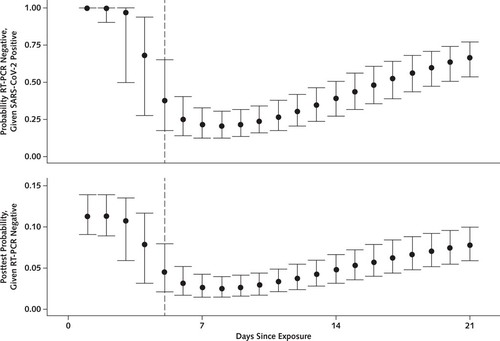
\includegraphics[width=15cm, height=6cm]{Images/RTPCR.jpg}
    %\decoRule
    \caption[RT-PCR Test Negative Rate]{Probability of having a negative RT-PCR test result given SARS-CoV-2 infection (top) and of being infected with SARS-CoV-2 after a negative RT-PCR test result (bottom), by days since exposure \cite{KLL+2020}}
    \label{fig:RT-PCR Test Negative Rate}
    \end{figure}
\vspace{-1em}
Another important factor considering the daily rising numbers are the delays in receiving the results for the RT-PCR test. This places extra strain on the medical professionals in terms of workload and makes it difficult for them to apply safety protocols on suspected patients.

Therefore, due to these aforementioned limitations of the real-time RT-PCR test, finding a safer, more accurate, and faster diagnosis mechanism is essential. Thus, making COVID-19 diagnosis using medical imagery an ideal alternative candidate.

\subsection{Medical Imagery} \label{medical imagery}
Medical Imagery such as X-rays and CT scans have proven to be a viable 
alternative to the RT-PCR test for COVID-19 detection 
due to the limitations mentioned above. The reduced exposure risks, and faster 
diagnosis time are also added benefits.

In this section, CT imaging features of the novel coronavirus 
shall be presented to lay a foundation for future sections 
where we illustrate how deep learning could learn these features 
and use it for automated real-time COVID-19 diagnosis.

A study conducted by Chung et al. on 21 symptomatic  
patients infected with coronavirus admitted to three hospitals in 
three provinces Guangdong, Jiangxi 
and Shandong respectively in China from January 18$^{th}$ 2020 to 
until January 27$^{th}$ 2020 aimed to identify potential imaging 
features of COVID-19 from CT scans reviewed and verified by two fellowship-trained 
cardiothoracic radiologists with approximately 5 years of experience each.

% After evaluation, the following common characteristics were observed:
% \begin{itemize}
%     \item Presence of Ground Glass Opacities (GGO's). 
%     \item Presence of Consolidation. 
%     \item Number of lobes affected by ground-glass or consolidative opacities. 
%     \item Degree of lobe involvement.
%     \item Presence of Nodules.
%     \item Presence of a Pleural Effusion. 
%     \item Presence of Thoracic Lymphadenopathy.
%     \item Presence of underlying lung disease such as Emphysema or Fibrosis.
%     \item Other abnormalities such as Cavitation, Reticulation, Interlobular Septal Thickening, Calcification, and Bronchiectasis.
%   \end{itemize}

The degree of lobe involvement was 
assessed and a "Total Severity Score" was assigned by summing up the each of the 
individual lob scores. Patients were also re-evaluated in order to study the 
progression of features by the same two radiologists \cite{CMA+2020}.

After evaluation, the following common characteristics tabulated in Table \ref{tab:CT Scan Review Results} were observed. Other abnormalities such as Cavitation, Reticulation, Interlobular Septal Thickening, Calcification, and Bronchiectasis were also assessed.
% \vspace{1em}
% The results of the above study are tabulated below: 

\begin{longtable}{| p{.65\textwidth} | p{.163\textwidth} |} 
\hline
\textbf{Finding} & \textbf{No. of Patients} \\
\hline
Ground-glass opacities and consolidation & \\
\quad Absence of both ground-glass opacities and consolidation & 3 (14\%)\\ 
\quad Presence of either ground-glass opacities or consolidation & 18 (86\%)\\
\quad Presence of ground-glass opacities without consolidation & 12 (57\%)\\
\quad Presence of ground-glass opacities with consolidation & 6 (29\%)\\
\quad Presence of consolidation without ground-glass opacities & 0 (0\%)\\ \hline
% No. of lobes affected & \\ \hline
% \quad 0 & 3 (14\%)\\ \hline
% \quad 1 & 1 (5\%)\\ \hline
% \quad 2 & 2 (10\%)\\  \hline
% \quad 3 & 3 (14\%)\\ \hline
% \quad 4 & 4 (19\%)\\ \hline
% \quad 5 & 8 (38\%)\\ \hline
Frequency of lobe involvement & \\ 
\quad Right Upper Lobe & 3 (14\%)\\
\quad Right Middle Lobe & 1 (5\%)\\
\quad Right Lower Lobe & 2 (10\%)\\
\quad Left Upper Lobe & 3 (14\%)\\ 
\quad Left Lower Lobe & 4 (19\%)\\ \hline
% Total lung severity score & \\ \hline
% \quad Mean & 9.9\\ \hline
% \quad Range & 0-19\\ \hline
Opacification distribution and pattern & \\ 
 \quad Rounded Morphology & 7 (33\%)\\ 
 \quad Linear Opacities & 3 (14\%)\\ 
 \quad Crazy-Paving Pattern & 4 (19\%)\\ 
 \quad Peripheral Distribution & 7 (33\%)\\  \hline
More than two lobes affected & 15 (71\%)\\ \hline
Bilateral lung disease & 16 (76\%)\\ \hline
%  \quad Cavitation & 0 (0\%)\\ \hline
%  Other Findings & \\ \hline
%  \quad Discrete Pulmonary Nodules & 0 (0\%)\\  \hline
%  \quad Pleural Effusion(s) & 0 (0\%)\\ \hline
%  \quad Lymphadenopathy & 0 (0\%)\\ \hline
%  \quad Pulmonary Emphysema & 0 (0\%)\\ \hline
%  \quad Pulmonary Fibrosis & 0 (0\%)\\    \hline
 
 \caption{Findings at Initial Chest CT Examination in 21 Patients  \cite{CMA+2020}.}

    \label{tab:CT Scan Review Results}
    \end{longtable}

% The patients with lung severity scores close to the maximum, which was 19, 
% were moved into the intensive care unit. One of the major observations was 
% that besides 3 out of the initial 21 patients, patients were observed to have 
% GGO's or consolidation.
% 
\vspace{-2.7em}
A follow-up chest CT scan was conducted on 8 of the initial 21 patients, within 
a range of 1 to 4 days. Only 1 patient out of the 8 had normal initial and 
follow-up CT scan results. 5 out of eight experienced mild progression in 
the lung characteristics, the remaining 2 displayed 
moderate progression. Fortunately, none of the patients experienced severe progression.

The primary observations from this study on 21 patients include GGO's 
found in 12 patients and consolidation in 6 patients. There is also a high possibility 
the virus affects more than two lobes with bilateral involvement. Other 
observations include rounded morphology detected in 7 patients, 
reticulation in 3 patients, and crazy-paving in 4 patients \cite{CMA+2020}.
% \\
%  \vspace{-2em}

\begin{figure}[H]
 \centering
 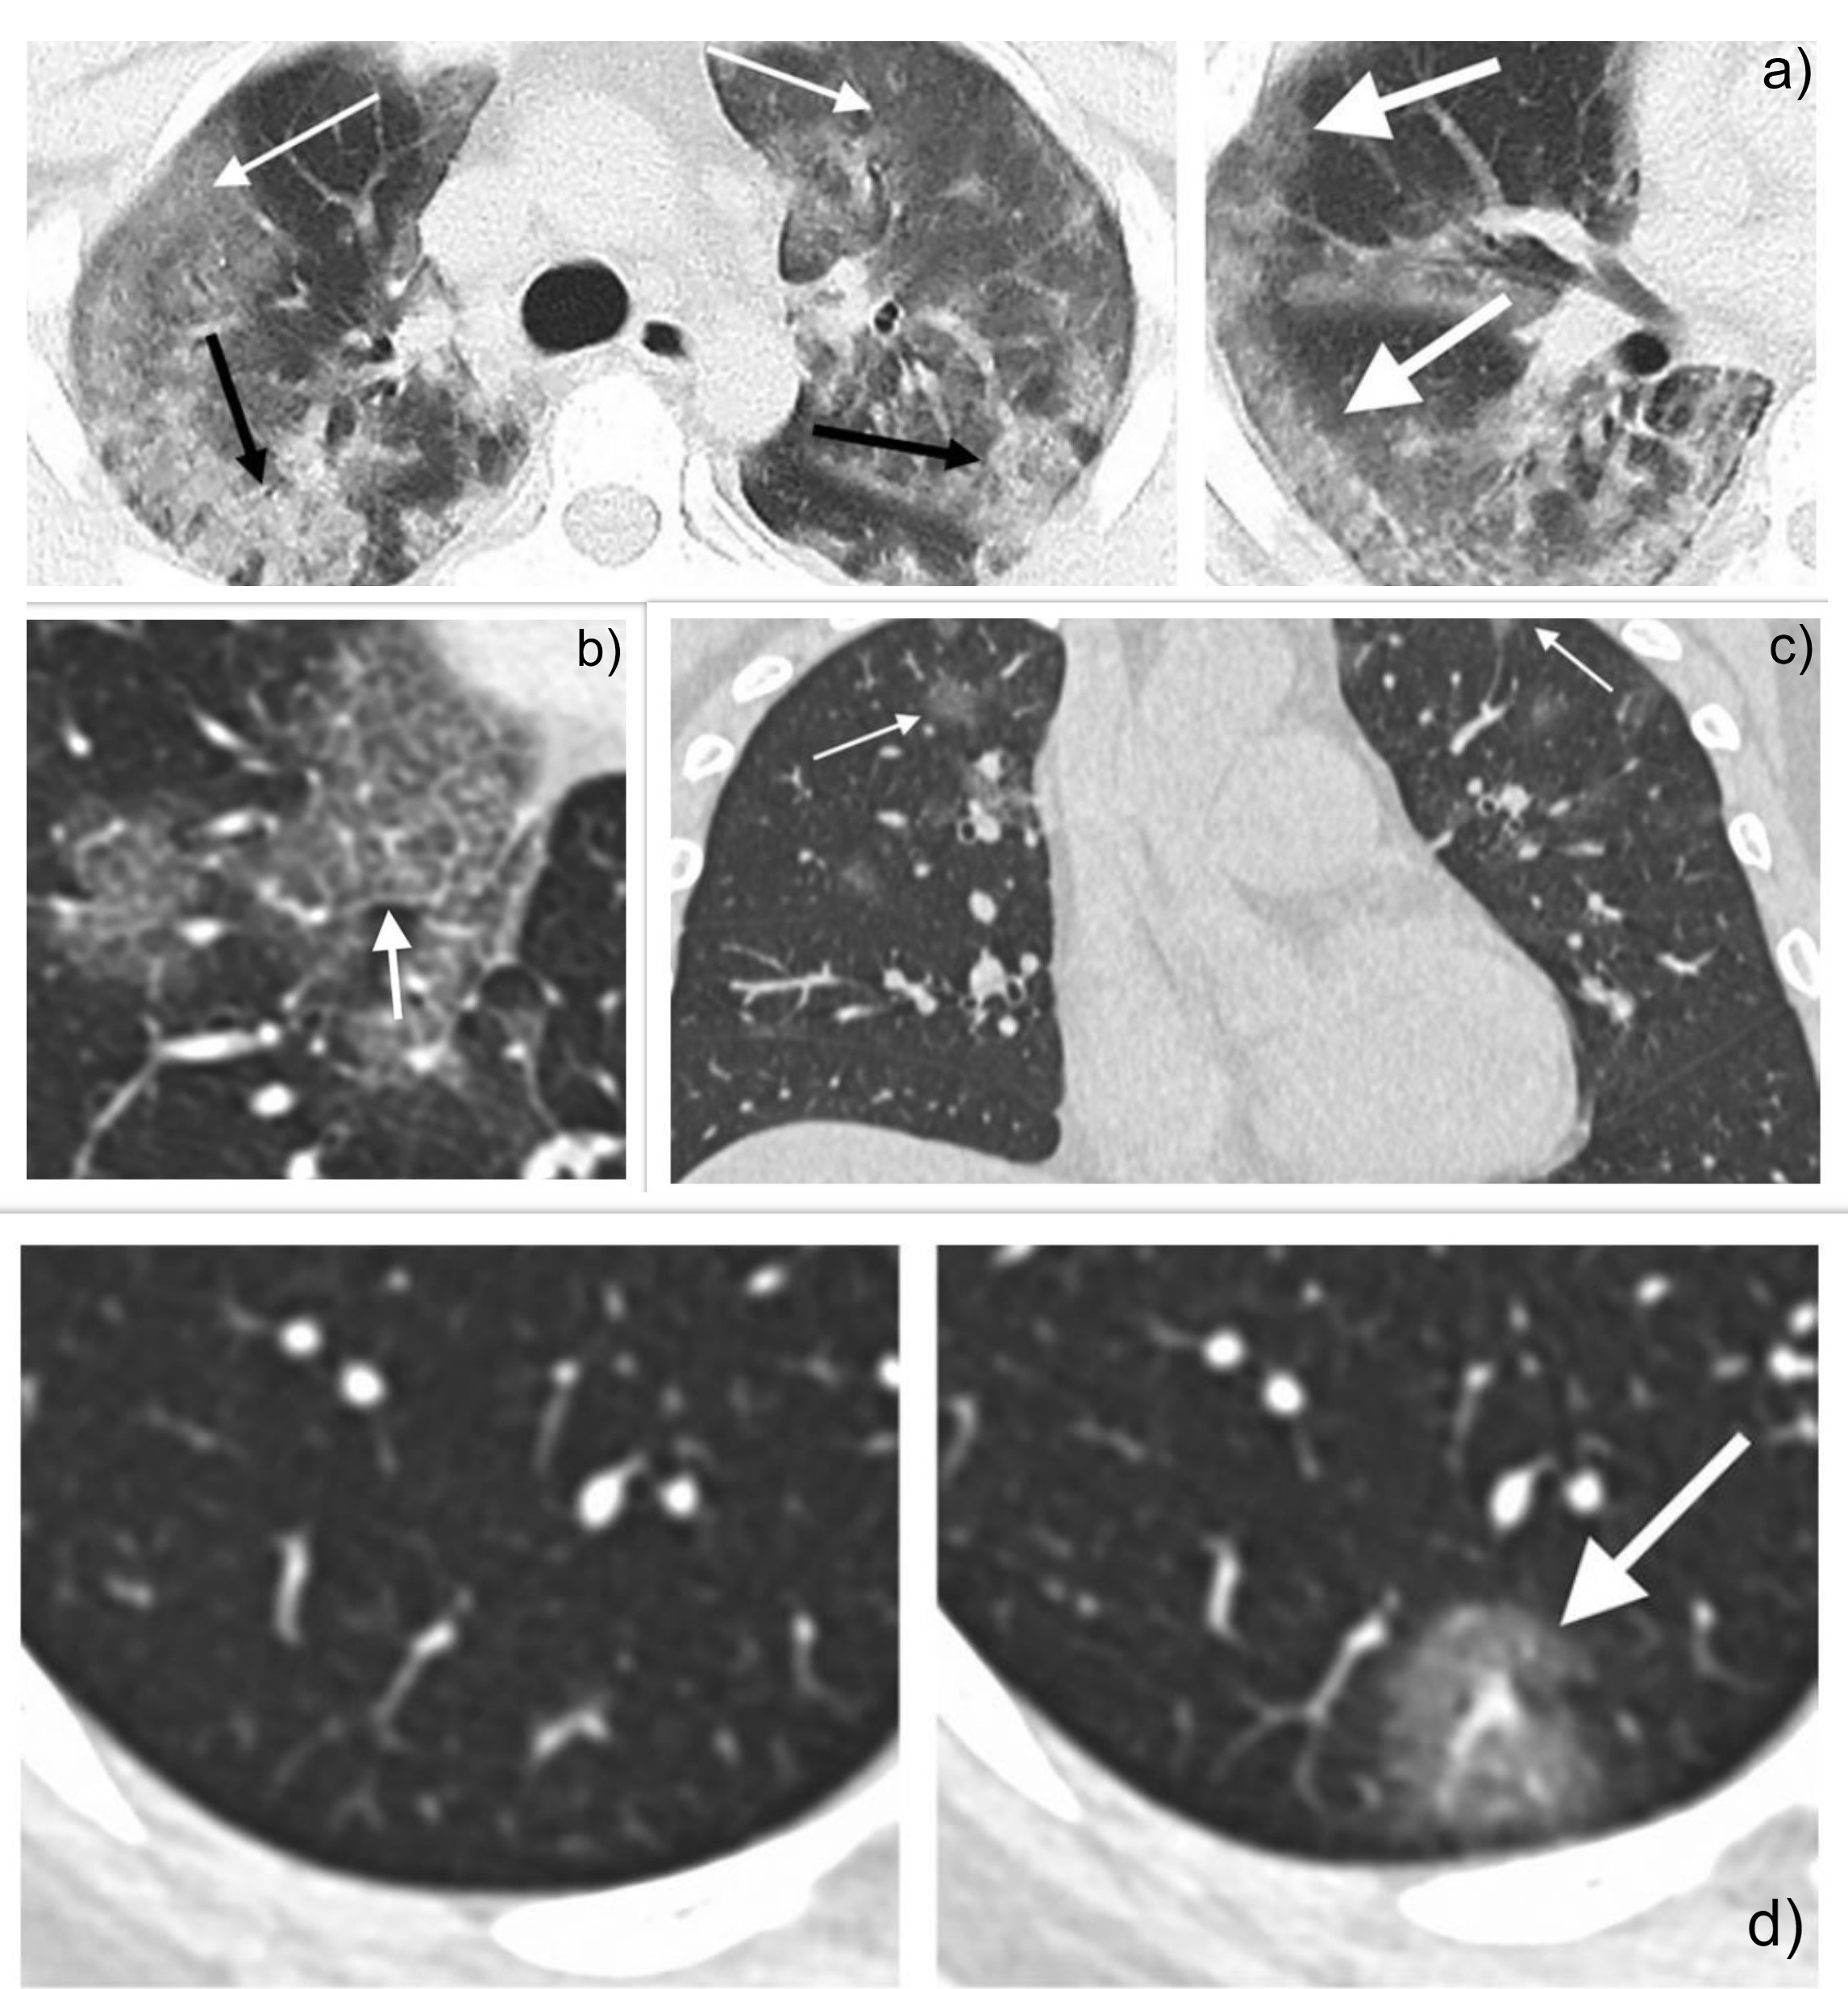
\includegraphics[width=15.5cm, height=12.5cm]{Images/CTScans2.jpg}
 %\decoRule
 \caption[CT Scan Images]{Observed lung CT Scan characteristics. a) White arrow indicates patchy GGO, and black arrow indicates consolidative pulmonary opacities. b) White arrow indicates GGO's with a rounded morphology. c)  White arrow indicates crazy-paving pattern, GGO and interlobular sepal thickening with intralobular lines. d) Follow-up CT scan progression. White arrow indicates new solitary, rounded, peripheral ground-glass lesion \cite{CMA+2020}.}
 \label{fig:CT Scan Image 1}
 \end{figure}
%  \vspace{-2em}
% \begin{figure}[H]
%  \centering
%  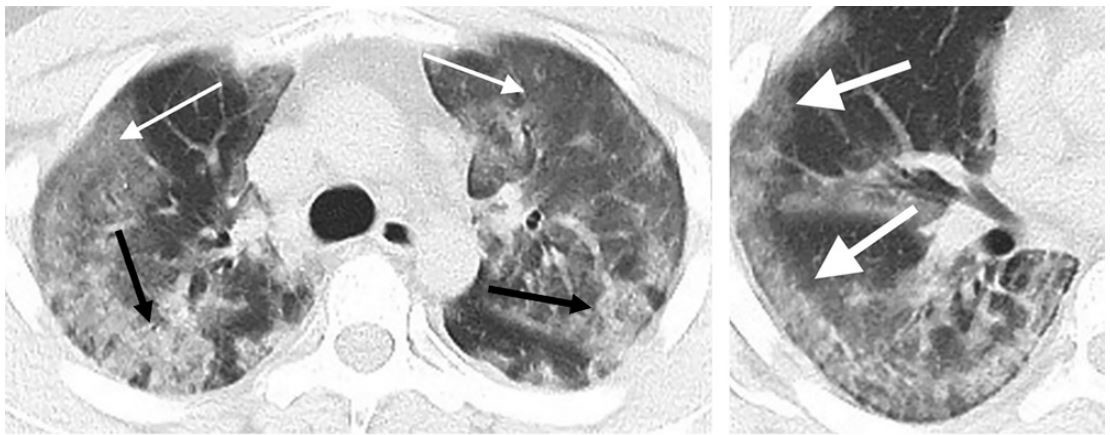
\includegraphics[width=15.5cm, height=5cm]{Images/CTScan1.JPG}
%  %\decoRule
%  \caption[CT Scan Image 1]{Observed lung CT Scan characteristics. White arrow indicates patchy GGO, and black arrow indicates consolidative pulmonary opacities \cite{CMA+2020}.}
%  \label{fig:CT Scan Image 1}
%  \end{figure}

% \begin{figure}[H]
% \centering
% 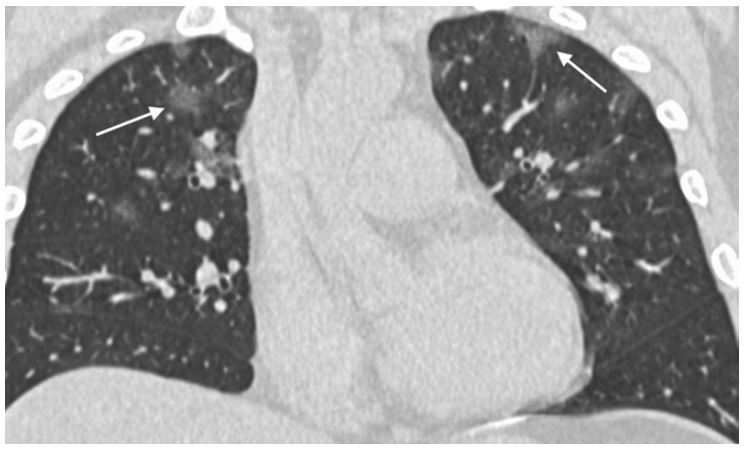
\includegraphics[width=15.5cm, height=5cm]{Images/CTScan2.JPG}
% %\decoRule
% \caption[CT Scan Image 2]{Observed lung CT Scan characteristics. White arrow indicates GGO's with a rounded morphology \cite{CMA+2020}.}
% \label{fig:CT Scan Image 2}
% \end{figure}
        
%  \begin{figure}[H]
%     \centering
%     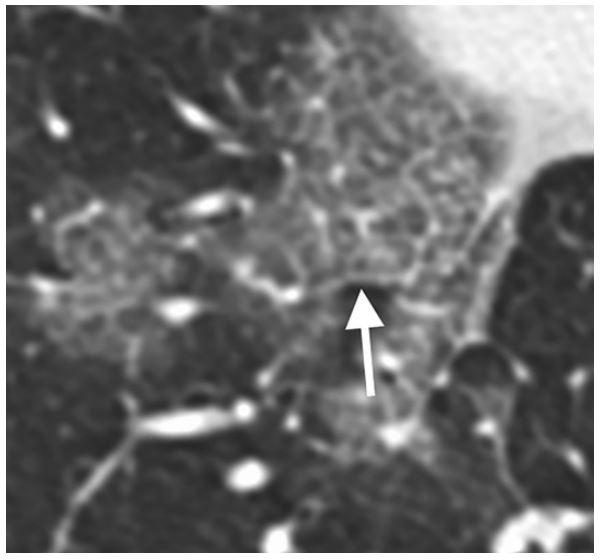
\includegraphics[width=15.5cm, height=5cm]{Images/CTScan3.JPG}
%     %\decoRule
%     \caption[CT Scan Image 3]{Observed lung CT Scan characteristics. White arrow indicates crazy-paving pattern, GGO and interlobular sepal thickening with intralobular lines  \cite{CMA+2020}.}
%     \label{fig:CT Scan Image 3}
%     \end{figure}

% \begin{figure}[H]
%     \centering
%     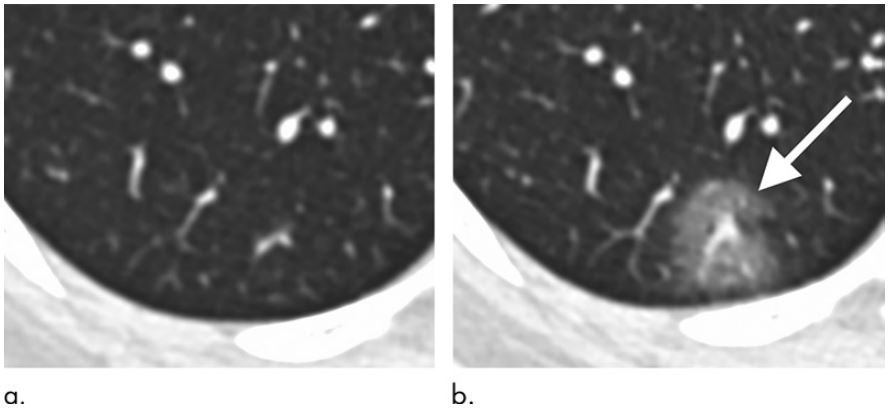
\includegraphics[width=15.5cm, height=6cm]{Images/CTScanProgression.JPG}
%     %\decoRule
%     \caption[CT Scan Progression]{Follow-up CT scan lung characteristics progression. White arrow indicates new solitary, rounded, peripheral ground-glass lesion \cite{CMA+2020}.}
%     \label{fig:CT Scan Image 4}
%     \end{figure}
\vspace{-2em}
One obvious limitation of this study is the relatively low number of 
patients, with only 8 out of 21 carrying out a follow-up CT scan. As this study
was conducted during the dawn of coronavirus, this number is certainly a 
very respective amount.

Another study by Morales et al. whose results are summarized in Appendix \ref{COVID-19 Lung Characteristics}, also observe similar lung characteristics. As we have now seen the prominent imaging characteristics of 
COVID-19, we shall now discuss how deep learning could learn these 
features and accurately diagnose patients with COVID-19 in real-time. 

\section{Deep Learning for COVID-19 Diagnosis}

The coronavirus global pandemic spreading rapidly all across the world have 
forced scientists and researchers to identify alternative 
diagnosis mechanisms in addition to the RT-PCR test to overcome 
its limitations. As we have seen in previous sections, 
medical imagery such as X-rays and CT scans have played a 
vital role in combating the rising numbers by saving 
valuable time in diagnosis and reducing virus exposure.

Deep learning techniques have further enhanced COVID-19 diagnosis 
using medical imagery due to its rapid detection capabilities, 
fully automated and efficient diagnosis workflow, 
and assisting medical practitioners by highlighting observed 
COVID-19 lung characteristics similar to 
features discussed in the section \ref{medical imagery}. A detailed overview of the modern CT and X-ray systems enabling automated diagnosis workflow ensuring minimal virus exposure can be found in Appendix \ref{Automated Diagnosis Workflow}.

% In this section, we will have a comprehensive discussion on how 
% deep learning techniques could accurately diagnose patients with COVID-19 by reviewing the methodologies used and the results 
% obtained by experiments and studies conducted across the world.

To identify the regions of interest (ROIs), segmentation of the 
lung CT or X-ray scans are a vital pre-requisite. The former produces 
high-quality 3D images for detecting COVID-19 whereas the latter involves 
the ribs being projected onto soft-tissues in 2D. 

As a result, segmentation 
in X-ray scans is more challenging as compared to CT scans. But on the other hand, 
X-ray scans are more widely accessible in medical facilities all across the world 
and are usually the first imaging modality used on patients suspected of COVID-19.

Keeping in mind these limitations, the next two subsections review the segmentation techniques using deep learning for both CT and X-rays respectively and 
discuss the results obtained.

\subsection{CT Based Diagnosis of COVID-19}
To identify the ROIs from a CT scan for diagnosis, deep learning 
techniques are extensively used. These techniques could be narrowed down 
to the three most prominent segmentation methods which are \textbf{U-Net} \cite{CXZ+2020, CYZ+2020, HLR+2020, YHQ+2020, GOM+2020, LLL+2020}, \textbf{UNet++} \cite{CJL+2020, JSB+2020}, and \textbf{VB-Net}  \cite{SFY+2020} respectively.

% \begin{itemize}
%     \item U-Net \cite{CXZ+2020, CYZ+2020, HLR+2020, YHQ+2020, GOM+2020, LLL+2020}
%     \item UNet++ \cite{CJL+2020, JSB+2020}
%     \item VB-Net \cite{SFY+2020}
% \end{itemize}

From section \ref{medical imagery}, we can infer that the main ROIs could be classified into 
two specific categories, which are lung-region and lung-lesion oriented 
methods. The latter is more of a challenge in terms of its detection as lesions 
could be in a variety of shapes and sizes, furthermore, locating its region 
also adds to the difficulty in identifying it.

The literature indicates U-Net architecture as most reliable in segmenting both lung regions and lesions in COVID-19 diagnosis 
applications. Designed by Ronneberger, U-Net as its name suggests has a U-shape architecture, 
such that it has a symmetric expansive and contracting path \cite{RFT2015}.

\begin{figure}[H]
    \centering
    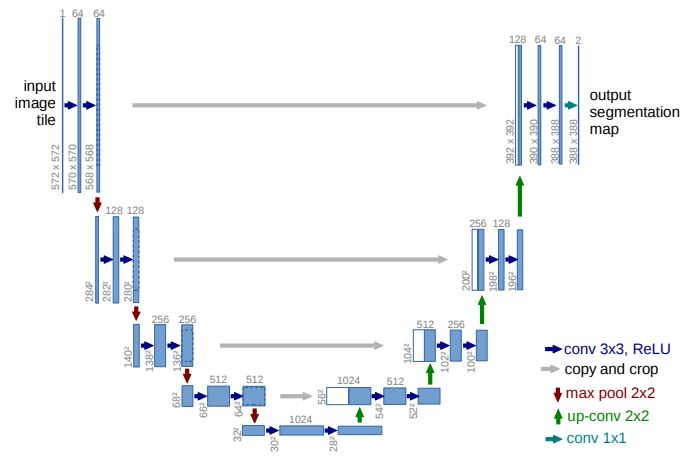
\includegraphics[height=6.5cm]{Images/UNet.JPG}
    %\decoRule
    \caption[U-Net Architecture]{A representation of the U-Net architecture \cite{RFT2015}}
    \label{fig:U-Net Architecture}
    \end{figure}
\vspace{-2em}
Various variants of the U-Net have been developed since its inception due to its high ability to learn visual semantics and therefore are suitable 
for many medical applications. They include the following:
\begin{itemize}
    \item \textbf{3D U-Net} - Replaces the conventional U-Net layers with 3D layers. \cite{SCS+2020}
    \item \textbf{V-Net} - Utilizes residual blocks as the convolutional block, network optimization carried out through Dice Loss. \cite{MNA+2020}
    \item \textbf{VB-Net} - Combination of V-Net with a bottle-neck structure. \cite{SFY+2020}
    \item \textbf{UNet++} - A more complex version of U-Net, inserts a nested convolutional structure between the expansive and contracting path. \cite{ZSM+2020}
    \item \textbf{Attention U-Net} - Integrates Attention Gates with U-Net architecture to focus on target structures of various shapes and sizes. \cite{OSF+2020}
\end{itemize}

% \vspace{-2em}
Identifying and labeling the training data for the purpose of COVID-19 diagnosis is often 
time consuming and labour intensive, especially the manual detection of lesions. Shan et al. proposes a workaround which involves the "human-in-the-loop" strategy, 
where radiologists play an integral part in the training process \cite{SFY+2020}. Another similar suggestion from Yue et al. was to allow the radiologists to provide initial seeds for the U-Net  model \cite{YHQ+2020}.

Zheng et al. suggests an alternative approach, where unsupervised methods are used to generate pseudo segmentation masks for images to overcome 
the labeling process and thus avoid its limitations. In addition to reviewing results of lung segmentation from the U-Net model, Zheng et al. also utilizes a 3D CNN to predict the probability of 
COVID-19 using images obtained as an input \cite{CXZ+2020}. With a 
dataset of 540 patients, 313 with COVID-19, and remaining without COVID-19 
are used for training and testing purposes. The model attains a sensitivity 
of 90.7\% and specificity 91.1\%.

The lung segmentation's obtained could be used for COVID-19 diagnosis and for the 
quantification of data. The literature mentioned in this section includes both of the 
objectives.

Li et al. conducted a multi-center study by distinguishing COVID-19 from community-acquired pneumonia \cite{LLL+2020}. A combination of U-Net and ResNet-50 was proposed with the former used to extract lung regions using pre-processed 2D slices. The latter along with shared weights between the 2D slices combined 
with max-pooling is used for COVID-19 diagnosis. This study utilizes a large dataset 
with 1296 COVID-19 patients, 1735 with community-acquired pneumonia, and 1325 
non-pneumonia patients. The model achieves a specificity of 96\% and sensitivity 
of 90\%.  

An AI system developed by Jin et al. for rapid COVID-19 diagnosis, involves the input to the classification model 
being the CT slices which have been segmented \cite{JSB+2020}. Instead of a 3D CNN, a ResNet-50 model was used for diagnosis
and UNet++ for lung segmentation and lesion identification. The model 
is trained on 1136 images, 723 COVID-19 positives, and 413 negatives and 
achieves sensitivity and specificity of 97.4\% and 92.2\% respectively.

As for the quantification of data, both Cao et al. \cite{CYZ+2020} and Huang et al. \cite{HLR+2020} monitor the longitudinal 
progression of COVID-19 using the CT segmentation of pulmonary opacities using the segmentation of 
the lung region and GGO. Therefore, the image segmentation obtained aids radiologists 
in infection identification, analysis, and diagnosis.

Most of the classification studies involve segregating COVID-19 patients 
from non-COVID-19 with most of the latter patients being segregated further 
into pneumonia and non-pneumonia subjects.

Chen et al. developed a UNet++ model which segments lung lesions 
\cite{CJL+2020} using CT images of 51 COVID-19 patients and 
55 patients with other diseases and diagnose patients with 95.2\% accuracy thus reducing the reading time of radiologists by 65\%. Given 
raw images to the model, prediction boxes displaying suspected regions were output,
after further extraction and filtering a logic linking of predictions was added, which 
aimed to aid radiologists in manual detection of the virus.

Jin et al. considers an alternative approach  
utilizing 2D Deeplab v1 and 2D ResNet-152 models for lung segmentation 
and lung-mask slice based classification of COVID-19 respectively \cite{JCW+2020}. The 
model achieves a respectable score of 94.1\% sensitivity and 95.5\% 
specificity using a dataset of 496 COVID-19 positive CT scan images.

The objective of the remaining studies besides COVID-19 diagnosis is its differentiation
with common pneumonia which primarily 
includes viral pneumonia. The main reason for this objective being the 
very similar radiological appearances of both the diseases.

Wang et al. classifies between COVID-19 and viral pneumonia using a 2D CNN model on delineated 
region patches \cite{WBX+2020}. Experiments were conducted on chest CT scans from 
44 COVID-19 and 55 pneumonia patients with external testing 
resulting in 79.3\% accuracy.

Experiments carried out by Song et al. employs OpenCV to segment 
2D slices which include lung regions \cite{SZL+2020}. The 3D chest CT images resulted in 
15 2D slices of complete lungs and each slice were fed into the deep learning based CT diagnosis system also called DeepPneumonia. A combination of 
a pre-trained ResNet-50 along with Feature Pyramid Network (FPN) which can 
extract specific ranked details from the images, coupled 
with an attention module to learn these extracted details were used to develop this model.

The dataset includes 88 COVID-19 patients, 101 bacterial pneumonia and 86 
healthy patients. The proposed model achieves a classification accuracy of 86\%.

Table \ref{tab:CT Image Segmentation Techniques} and \ref{tab:COVID-19 Diagnosis Applcations} summarizes all the COVID-19 image segmentation 
applications mentioned in this section,
and the results of diagnosis experiments conducted across various 
medical facilities. An extended version of Table \ref{tab:CT Image Segmentation Techniques} can be found in Appendix \ref{CT Image Segmentation Techniques}.
\vspace{1em}

\begin{longtable}{| p{.25\textwidth} | p{.15\textwidth} |  p{.25\textwidth} |} 

    \hline
\textbf{Study} & \textbf{Method} & \textbf{Target ROI}  \\
\hline
\multirowcell{2}{Zheng et al. \cite{CXZ+2020}} & \multirowcell{2}{U-Net} & \multirowcell{1}{Lung} \\ \cline{3-3}  & & \multirowcell{1}{Lesion}  \\ \hline
\multirowcell{2}{Cao et al. \cite{CYZ+2020}} & \multirowcell{2}{U-Net} &  \multirowcell{1}{Lung} \\ \cline{3-3} & & \multirowcell{1}{Lesion} \\ \hline
\multirowcell{3}{Huang et al. \cite{HLR+2020}} & \multirowcell{3}{U-Net} & \multirowcell{1}{Lung} \\ \cline{3-3} & & \multirowcell{1}{Lung Lobes} \\ \cline{3-3} & &  \multirowcell{1}{Lesion}  \\ \hline
\multirowcell{2}{Yue et al. \cite{YHQ+2020}} & \multirowcell{2}{U-Net} & \multirowcell{1}{Lung Lobes} \\ \cline{3-3} & & \multirowcell{1}{Lesion} \\ \hline
\multirowcell{2}{Gozel et al. \cite{GOM+2020}} & \multirowcell{2}{U-Net} & \multirowcell{1}{Lung} \\ \cline{3-3}  & & \multirowcell{1}{Lesion} \\ \hline
% \multirowcell{4}{Shan et al. \cite{SFY+2020}} & \multirowcell{4}{VB-Net} & \multirowcell{4}{Diagnosis} & \multirowcell{1}{Lung} \\ \cline{4-4} & & & \multirowcell{1}{Lung Lobes} \\ \cline{4-4} &  & & \multirowcell{1}{Lung Segments} \\ \cline{4-4} & & & \multirowcell{1}{Lesion}\\ \hline
% \multirowcell{1}{Li et al. \cite{LLL+2020}} & \multirowcell{1}{U-Net} & \multirowcell{1}{Diagnosis} & \multirowcell{1}{Lesion} \\ \hline
% \multirowcell{1}{Chen et al. \cite{CJL+2020}} & \multirowcell{1}{UNet++} & \multirowcell{1}{Diagnosis} & \multirowcell{1}{Lesion} \\ \hline
% \multirowcell{2}{Jin et al. \cite{JSB+2020}} & \multirowcell{2}{UNet++} & \multirowcell{2}{Diagnosis} & \multirowcell{1}{Lung} \\ \cline{4-4} & & &  \multirowcell{1}{Lesion}\\ \hline
\multirowcell{4}{Tang et al. \cite{TLX+2020}} & \multirowcell{4}{Commercial\\Software} & \multirowcell{1}{Lung} \\ \cline{3-3}  & & \multirowcell{1}{Lesion} \\ \cline{3-3}  & & \multirowcell{1}{Trachea} \\ \cline{3-3}  & & \multirowcell{1}{Bronchus}\\ \hline
% \multirowcell{3}{\cite{SCN+2020}} & \multirowcell{3}{Threshold-based\\Region Growing\\\cite{LBC+2020}} & Lesion \\ \hline

\caption{CT Image Segmentation Techniques in COVID-19 Quantification Applications \cite{SFJ+2020}}

    \label{tab:CT Image Segmentation Techniques}
    \end{longtable}
    
% \vspace{-1em}

\begin{longtable}{| p{.25\textwidth} | p{.20\textwidth} | p{.15\textwidth} | p{.20\textwidth} |} 

    \hline
\textbf{Study} & \textbf{Subjects} & \textbf{Method} & \textbf{Result}  \\
\hline
\multirowcell{2}{Zheng et al. \cite{CXZ+2020}} & \multirowcell{1}{313 COVID-19} & \multirowcell{1}{U-Net} & \multirowcell{1}{90.7\% (Sens.)} \\ \cline{2-4} & \multirowcell{1}{229 Others} & \multirowcell{1}{CNN} & \multirowcell{1}{91.1\% (Spec.)}\\ \hline
\multirowcell{3}{Li et al. \cite{LLL+2020}} & \multirowcell{1}{468 COVID-19} & \multirowcell{3}{ResNet-50} & \multirowcell{1}{90.0\% (Sens.)} \\ \cline{2-2} \cline{4-4}  & \multirowcell{1}{1551 CAP} & & \multirowcell{1}{96.0\% (Spec.)} \\ \cline{2-2} \cline{4-4} & \multirowcell{1}{1445 Non-pneu.} && \multirowcell{1}{0.95 (AUC.)}\\ \hline
\multirowcell{2}{Chen et al. \cite{CJL+2020}} & \multirowcell{1}{51 COVID-19} & \multirowcell{2}{UNet++} & \multirowcell{1}{100\% (Sens.)} \\ \cline{2-2} \cline{4-4} & \multirowcell{1}{55 Others} &  & \multirowcell{1}{93.6\% (Spec.)} \\ \hline
\multirowcell{2}{Jin et al. \cite{JSB+2020}} & \multirowcell{1}{723 COVID-19} & \multirowcell{2}{UNet++} & \multirowcell{1}{97.4\% (Sens.)} \\ \cline{2-2} \cline{4-4} & \multirowcell{1}{413 Others} &  & \multirowcell{1}{92.2\% (Spec.)} \\ \hline
\multirowcell{2}{Jin et al. \cite{JCW+2020}} & \multirowcell{1}{496 COVID-19}& \multirowcell{2}{CNN} & \multirowcell{1}{94.1\% (Sens.)} \\ \cline{2-2} \cline{4-4} & \multirowcell{1}{1385 Others} &  & \multirowcell{1}{95.5\% (Spec.)} \\ \hline
\multirowcell{3}{Song et al. \cite{SZL+2020}} & \multirowcell{1}{88 COVID-19} & \multirowcell{3}{ResNet-50} & \multirowcell{3}{86.0\% (Acc.)} \\ \cline{2-2}  & \multirowcell{1}{100 Bac. Pneu.} &  & \\ \cline{2-2}  & \multirowcell{1}{86 Normal} &  & \\ \hline
\multirowcell{2}{Wang et al. \cite{WBX+2020}} & \multirowcell{1}{44 COVID-19} & \multirowcell{2}{CNN} & \multirowcell{2}{79.3\% (Acc.)} \\ \cline{2-2} & \multirowcell{1}{55 Vir. Pneu.} &  & \\ \hline
\caption{COVID-19 Diagnosis Applications and their results from CT Image Segmentation \cite{SFJ+2020}}
\label{tab:COVID-19 Diagnosis Applcations}
    \end{longtable}
\begin{center} 
\vspace{-2em}
\textcolor{red}{* } Bac. - Bacterial, Vir. - Viral, Pneu. - Pneumonia \end{center}
As we have seen, the above studies result in promising diagnosis outcomes. Therefore, 
COVID-19 diagnosis with CT images could facilitate early detection of the coronavirus 
and also reduce the high exposure rates between patients and medical professionals.

\subsection{X-ray Based Diagnosis of COVID-19}
X-rays are most often the first imaging modality used on suspected patients, due 
to its wide availability in most clinics and medical facilities. As seen in section \ref{medical imagery},
radiological signs include GGOs, consolidation, and opacification.

In order to detect these abnormalities in lung X-ray scans, three popular 
architecture's are used across various studies which are \textbf{ResNet} \cite{ZXS+2020}, \textbf{ResNet-50} \cite{AKP2020}, and \textbf{CNN} \cite{GHT2020, LWA2020}.
% \vspace{-2em}
% \begin{itemize}
%     \item ResNet \cite{ZXS+2020}
%     \item ResNet-50 \cite{AKP2020}
%     \item CNN \cite{GHT2020, LWA2020}
% \end{itemize}
% \vspace{-2em}

\begin{figure}[H]
    \centering
    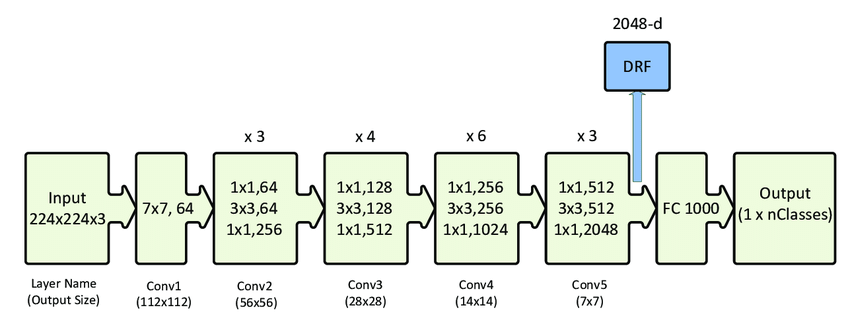
\includegraphics[width=15cm, height=3.5cm]{Images/ResNet.png}
    %\decoRule
    \caption[ResNet-50 Architecture]{ResNet-50 architecture with residual units \cite{MOB+2020}}
    \label{fig:ResNet-50 Architecture}
    \end{figure}
\vspace{-2em}
X-rays despite, as mentioned previously, being the first imaging modality for 
patients suspected with COVID-19 is less sensitive than 3D chest CT images. 
Anomalous chest radiographs are found in 69\% of the patients initially during 
admission and this number increases to 80\% after a certain period 
once hospitalized \cite{WLA+2020}.

To estimate the uncertainty in COVID-19 prediction Ghoshal et al. \cite{GHT2020} proposes 
a Bayesian CNN. X-rays of 70 COVID-19 patients are obtained 
from Cohen et al. \cite{JMD2020} and others from Kaggle's chest X-ray images. Bayesian 
inference improves the detection accuracy of the model from 85.7\% to 92.9\% from 
the experiments conducted by the authors.

Narin et al. experiments with three deep learning models 
i.e., ResNet-50, InceptionV3 and Inception-ResNetV2 respectively, with the objective 
to detect COVID-19 from X-ray images  \cite{AKP2020}. The dataset includes X-rays from 50 COVID-19 patients and 50 normal scans.
 The results indicate that ResNet-50 achieves highest accuracy with 98\% followed by InceptionV3 which 
attains 97\%.

Zhang et al. also suggest a ResNet based model for COVID-19 detection \cite{ZXS+2020}. 
But the model aims to achieve two objectives, one for COVID-19 classification and another for anomaly detection. The experiment was conducted on a dataset containing X-rays from 
70 COVID-19 patients and 1008 other X-rays. The anomaly detection score in-turn optimizes the COVID-19 
classification score which reaches 96\% from the experiments conducted by the authors.

Wang et al. proposes a deep CNN based model (COVID-Net) and
achieves a testing accuracy of 83.5\%  \cite{LWA2020}. The dataset used for the study include X-rays from 
patients diagnosed with both Bacterial and Viral Pneumonia. More specifically, 
45 COVID-19 positive, 931 Bacterial Pneumonia, 660 Viral Pneumonia, and 1203 normal X-rays.

Table \ref{tab:X-ray Image Segmentation Techniques} summarizes the results obtained by the experiments discussed in this section.
% \\
\begin{longtable}{| p{.30\textwidth} | p{.20\textwidth} | p{.15\textwidth} | p{.15\textwidth} |} 

    \hline
\textbf{Study} & \textbf{Subjects} & \textbf{Method} & \textbf{Result}  \\
\hline
\multirowcell{2}{Ghoshal et al. \cite{GHT2020}} & \multirowcell{1}{70 COVID-19} & \multirowcell{2}{CNN} & \multirowcell{2}{92.9\% (Acc.)} \\ \cline{2-2} & \multirowcell{1}{Others} & &\\ \hline
\multirowcell{2}{Zhang et al. \cite{ZXS+2020}} & \multirowcell{1}{70 COVID-19} & \multirowcell{2}{ResNet} & \multirowcell{1}{96.0\% (Sens.)} \\ \cline{2-2} \cline{4-4} & \multirowcell{1}{1008 Others} &  &  \multirowcell{1}{70.7\% (Spec.)} \\ \hline
\multirowcell{2}{Narin et al. \cite{AKP2020}} & \multirowcell{1}{50 COVID-19} & \multirowcell{2}{ResNet-50} & \multirowcell{2}{98.0\% (Acc.)} \\ \cline{2-2} & \multirowcell{1}{50 Normal} & &\\ \hline
\multirowcell{4}{Wang et al. \cite{LWA2020}} & \multirowcell{1}{45 COVID-19} & \multirowcell{4}{CNN} & \multirowcell{4}{83.5\% (Acc.)} \\ \cline{2-2} & \multirowcell{1}{931 Bac. Pneu.} &  & \\ \cline{2-2} &  \multirowcell{1}{660 Viral Pneu.} && \\  \cline{2-2} &  \multirowcell{1}{1203 Normal} && \\ \hline
\caption{X-ray Image Segmentation Techniques in COVID-19 Diagnosis Applications \cite{SFJ+2020}}

    \label{tab:X-ray Image Segmentation Techniques}
    \end{longtable}
\vspace{-2em}
\begin{center}\textcolor{red}{* } Acc. - Accuracy, Sens. - Sensitivity, Spec. - Specificity \end{center}

As seen in the above studies on X-ray images, the classification of COVID-19 from other Pneumonia seems 
to be a repeating objective. The major limitation involves the lack of data available as 
currently there exist two online datasets with 70 images from COVID-19 patients, therefore 
the generalizability and stability of the model are yet to be evaluated.

\subsection{Interpreting Deep Learning Results}
\label{Interpreting Deep Learning Results}
Deep learning techniques are often regarded as "Black Boxes" concerning 
its training and classification mechanisms. In medical applications such as this topic where we 
aim to diagnose patients with COVID-19 in real-time, understanding the reasoning behind the model's prediction 
is of utmost importance. 

More than just an additional insight, visualization of distinct features 
from the lung segmentation images would allow radiologists to cross-check their findings with that of the deep 
learning model and thus allow for an even better and reliable diagnosis.

Saliency methods are a set of popular and powerful tools which allow researchers 
to analyze and understand deep learning decisions \cite{AGM+2018}. 
Various interpretation methods exist in deep learning with a few of them 
mentioned below:
\begin{itemize}
    \item \textbf{Saliency Map} - Estimates specific parts of the image which contributes to highest layer activation \cite{ZMF2013}.
    \item \textbf{Class Activation Mapping (CAM)} - Averages and adds the activation's of each feature map (Global Average Pooling) and uses this to highlight important regions \cite{ZKL+2015}.
    \item \textbf{Gradient-Weighted CAM (Grad-CAM)} - Calculates the gradient of the classification score with respect to the convolutional features \cite{RCD+2017}.
\end{itemize}

The saliency maps shown in Figure \ref{fig:X-ray images and their corresponding heat maps} and \ref{fig:Saliency Maps displaying COVID-19 lung characteristics in CT and X-ray scans} highlight those regions in the lungs 
which as discussed in Section \ref{medical imagery}, exhibit the most common characteristics 
in patients diagnosed with COVID-19. 
GGO's, consolidations, lesions, and crazy-paving patterns are some of the 
more contributing features for diagnosis purposes by the 
deep learning model as indicated by the saliency maps.

    \begin{figure}[H]
    \centering
    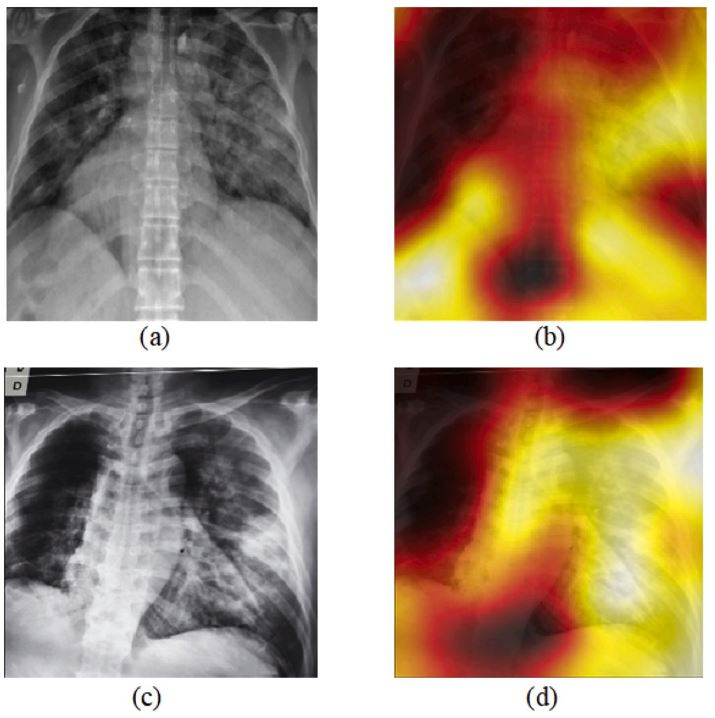
\includegraphics[width=15cm, height=6cm]{Images/Saliency4.JPG}
    %\decoRule
    \caption[X-ray Heat Map]{X-ray images and the corresponding heat maps \cite{OTY+2020}}
    \label{fig:X-ray images and their corresponding heat maps}
    \end{figure}




% Below shown are some saliency maps observed across multiple studies:
\begin{figure}[H]
    \centering
    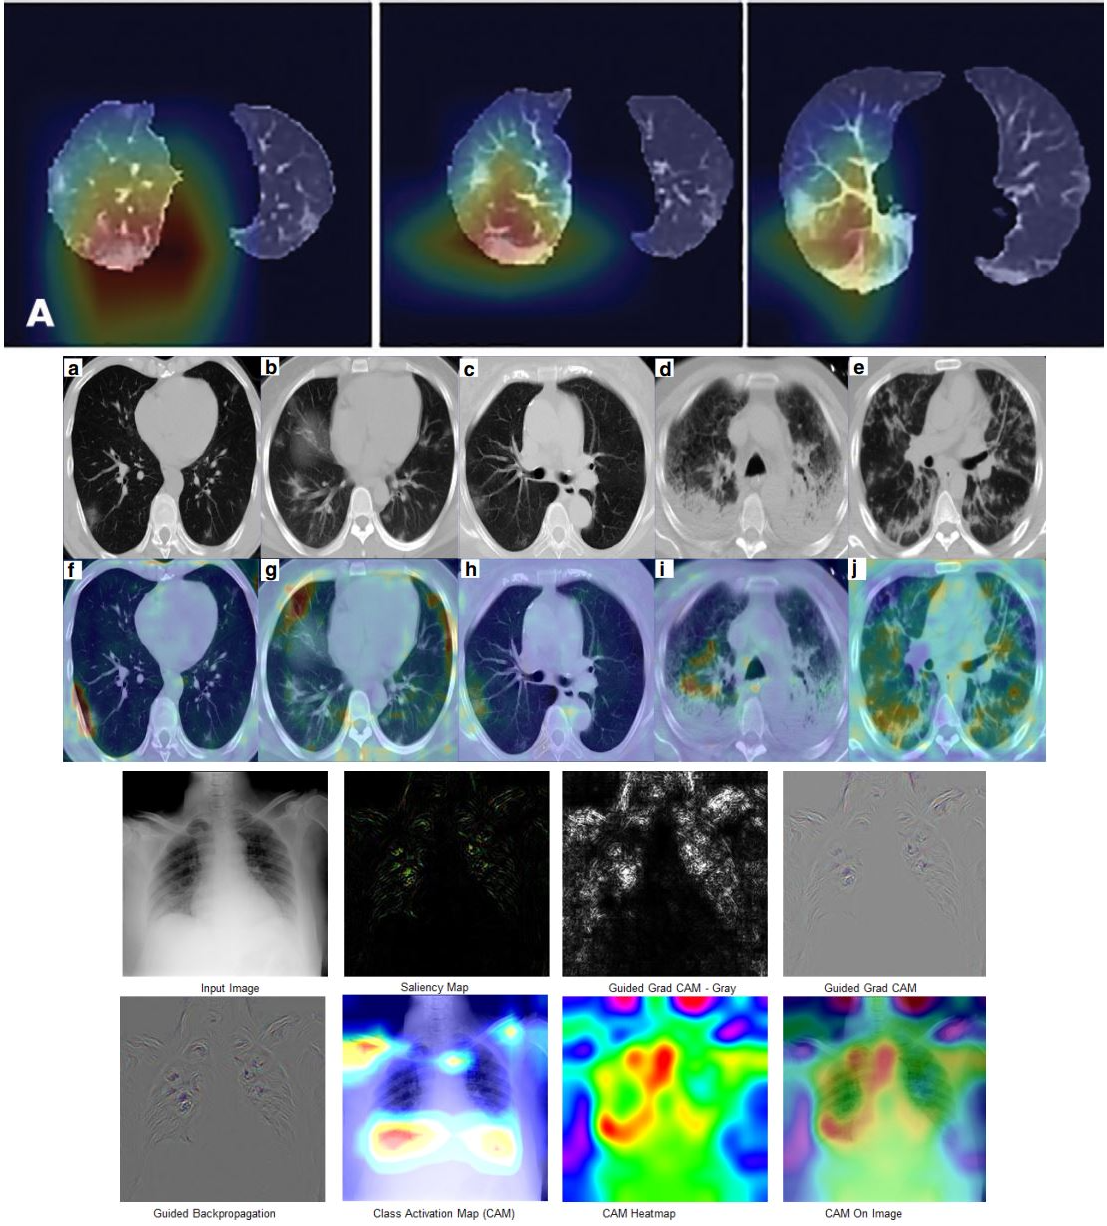
\includegraphics[width=15.5cm, height=12cm]{Images/Saliency Maps.png}
    %\decoRule
    \caption[Attention Heat Map]{Saliency Maps displaying COVID-19 lung characteristics in CT and X-ray scans \cite{LLL+2020} \cite{GHT2020} \cite{HSX+2020}}
    \label{fig:Saliency Maps displaying COVID-19 lung characteristics in CT and X-ray scans}
    \end{figure}
    

\vspace{-2em}
% \begin{figure}[H]
%     \centering
%     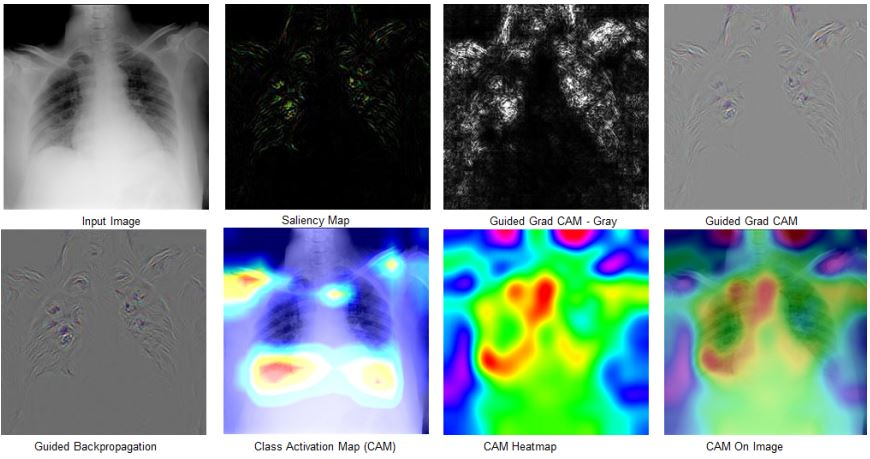
\includegraphics[width=15cm, height=5.5cm]{Images/Saliency.JPG}
%     %\decoRule
%     \caption[X-ray Saliency Map]{Saliency Map displaying COVID-19 lung characteristics in X-rays \cite{GHT2020}}
%     \label{fig:Saliency Map displaying COVID-19 lung characteristics in X-rays}
%     \end{figure}

%     \begin{figure}[H]
%         \centering
%         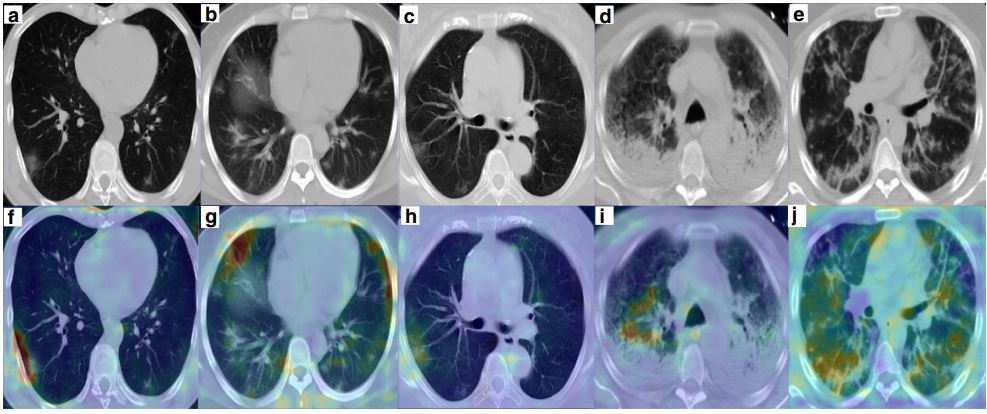
\includegraphics[width=15cm, height=5.5cm]{Images/Saliency2.JPG}
%         %\decoRule
%         \caption[CT Scan Saliency Map]{Saliency Map displaying COVID-19 lung characteristics in CT scans \cite{HSX+2020}}
%         \label{fig:Saliency Map displaying COVID-19 lung characteristics in CT scans}
%         \end{figure}

% The saliency maps highlight those regions in the lungs 
% which as discussed above, exhibit the most common characteristics 
% in patients diagnosed with COVID-19. 
% GGO's, consolidations, lesions, and crazy-paving patterns are some of the 
% more contributing features for diagnosis purposes by the 
% deep learning model as indicated by the saliency maps.

The results of saliency maps are therefore, in direct 
correlation with studies shown above which displays 
the most repeating COVID-19 lung characteristics. This provides 
additional assistance and assurance to radiologists who during 
diagnosis, look to identify the same lung characteristics.

% \vspace{-1em}
\section{Discussion}
The integration of AI techniques in medical research has 
just scratched the surface. We have discussed many studies 
which have experimented on fully automated COVID-19 
diagnosis employing deep learning methods and have 
yielded respectable results. But as mentioned, this is 
only the beginning and medical industry is due for a 
breakthrough soon. 

% \vspace{-1em}
\subsection{Overview of COVID-19 Applications}

Among many medical applications, where AI could potentially 
optimize and improvise standard procedures, automated 
imaging acquisition workflows as discussed previously, seem to be at the forefront. The overall efficiency of scanning procedure 
whether it be CT or X-rays could be enhanced and as a direct result, 
exposure to transferable viruses such as the coronavirus could be 
decreased, thus protecting medical professionals. 

% Besides protecting medical professionals, reducing patient 
% exposure to X-rays is also important. Calculating the right amount of radiation 
% to be used via body region thickness of the patient, finding an optimal patient position without technician intervention by automated calculation of 
% scan range and centering are promising AI-empowered solutions.

Section \ref{Interpreting Deep Learning Results} discusses Class Activation Mapping (CAM) which is a conventional 
technique to focus on prominent pixels or regions which lead to a 
resultant classification. Studies which have utilized this technique 
for COVID-19 diagnosis have seen a close correlation between the patterns 
identified by radiologists and the regions highlighted by the model therefore 
ensuring the reliability of the predictions given by the model.

Explainable Artificial Intelligence (XAI) methods \cite{ADD+2020, FSA+2020} are a recent addition 
to deep learning interpretability techniques which provides a finer localization 
map and exhibits more intricate details when compared to 
Class Activation Mapping (CAM) techniques.
% \vspace{-1em}
\subsection{Critical Review}

Using medical imagery for disease diagnosis has variety of applications, for example, 
diagnosing COVID-19 as seen through experiments conducted by multiple studies. But one noticeable caveat is the observed negative radiological signs during preliminary stages of the disease. This could have critical consequences in real-life circumstances especially amid a global pandemic.

% Overfitting of the results is very common in medical applications due to the lack of data available. Studies that involve AI techniques for segmentation and disease diagnosis are often hampered by this limitation. Therefore, to generalize the results obtained from a study, the availability of a respectable number of data is essential.

Many studies mentioned above use U-Net architecture for lung segmentation and variants of CNN's such as ResNet and ResNet-50 for COVID-19 diagnosis. One of the limiting factors of AI-based experiments is the difficulty in extracting the reasons as to why the deep learning model resulted in a certain classification. 

COVID-19 applications employing deep learning often require accurate 
labeling of data, but this task often is very time-consuming and medical 
professionals due to the rising numbers often would not be able to carry out 
this procedure. This leads to incomplete and inaccurate labeling of data which 
proves to be an additional challenge to deep learning models who train on this 
dataset and therefore result in an incorrect diagnosis.

Exploiting unsupervised training techniques \cite{NVF+2018, DGE2015} or exploring transfer learning methods \cite{TFK+2018}
where filters applied on a completely different dataset could be 
reused for COVID-19 applications are viable options to mitigate the above labeling 
complication.

As the coronavirus was declared a global pandemic fairly recently in early 2020, limited 
follow-up studies exist to identify treatment mechanisms and 
evaluating diagnosis tools. Few studies such as from Chung et al. \cite{CMA+2020}, mentioned earlier 
did in fact carry out follow-up CT scans to recognize progression patterns from 
segmented lung images, but due to the lack of participants when compared to the 
the initial version, the results obtained could not be reliably applied in the real world.

% Applying the findings obtained and methods carried out from 
% experiments conducted on related studies similar to COVID-19 diagnosis 
% would be the ideal path to take during this stage of the pandemic. 
% Especially from various pneumonia diseases as we have seen earlier to have similar radiological observations as that of the coronavirus. Deep learning 
% techniques employed for the diagnosis of pneumonia could also be replicated for 
% COVID-19 diagnosis.

% Applying the findings obtained and methods carried out from 
% experiments conducted on related studies similar to COVID-19 diagnosis 
% would be the ideal path to take during this stage of the pandemic. 
Tracking of COVID-19 patients is essential for containing 
the spread of the virus. Therefore medical facilities should enforce 
strict patient follow-up protocols carrying out long-term monitoring and capturing 
progression data which could be used by studies to further develop their models 
and deploy them in the real world. 

% \vspace{-1em}
\section{Conclusion and Research Questions}
The coronavirus has affected millions of lives throughout the world. 
Front-line workers combat the virus tirelessly to counter 
the rapidly rising numbers daily. In this chapter, we have discussed 
how deep learning could provide a safe, efficient and accurate 
workflow for COVID-19 diagnosis and be a suitable alternative to 
the RT-PCR test.

% AI-empowered techniques starting with automated scanning workflow 
% with the objective of reducing virus and radiation exposure for 
% the technicians and patients respectively, followed by two prominent 
% imaging modalities, i.e., CT and X-ray could play a pivotal role in 
% COVID-19 diagnosis.

It is important to couple the results obtained 
using the same imaging workflow discussed in this chapter, with clinical 
observations and laboratory results to provide reliable COVID-19 diagnosis.
From the experiments and studies discussed, it is safe to conclude 
that AI if utilized effectively could play a vital role in 
accurate diagnosis and analysis of COVID-19, and therefore potentially 
save precious lives and ultimately lead to our victory against the coronavirus
global pandemic.
\vspace{-1em}
\subsection*{Research Questions}
Based on the gaps we identified in this chapter, we plan to answer the following research questions:
%Upon project completion we aim to find answers to the following questions after applying  suitable evaluation strategies:

\begin{enumerate}
  \item Is there a correlation between the ROIs detected by the deep learning model and the lung characteristics observed on COVID-19 patients?
  \item Are the results obtained by the deep learning approach better when compared to the standard RT-PCR test?
  \item Is it feasible to deploy and utilize the deep learning model in medical facilities and laboratories for rapid real-time COVID-19 diagnosis?
\end{enumerate} 
% Chapter Template

\chapter{Requirements Analysis and Evaluation Strategy} % Main chapter title
\label{Requirements Analysis}
\label{ChapterX} % Change X to a consecutive number; for referencing this chapter elsewhere, use \ref{ChapterX}

%----------------------------------------------------------------------------------------
%	SECTION 1
%----------------------------------------------------------------------------------------

This chapter provides an insight into the project requirements followed by demonstrating the project implementation workflow, UI wireframe, data collection, and processing methodology, and concludes with an evaluation strategy.

\section{Requirements Analysis}
This section identifies and outlines the functional and non-functional requirements pertaining to this project. The priority 
of each of these requirements are ranked according to the MSCW prioritization technique. The following color-scheme 
indicates the respective ranking order:

\begin{itemize}
  \item \colorbox{green}{\textbf{Must Have (M)}} - These requirements are fundamental to achieve the aim of this project.
  \item \colorbox{cyan}{\textbf{Should Have (S)}} - These requirements are important to the project but not vital and could be achieved in the long run.
  \item \colorbox{yellow}{\textbf{Could Have (C)}} - These requirements are not fundamental to achieve the aim of this project but would be an added benefit if accomplished.
  \item \colorbox{pink}{\textbf{Want To Have (W)}} - These requirements would be prioritized in later releases of the project.
\end{itemize}

\subsection{Functional and Non-Functional Requirements}
The Functional Requirements (FR's) describes the essential components, purpose, and objectives of this project.
Table \ref{tab:Functional Requirements} tabulates the FR's along with a brief description for the same and its priority according to MSCW prioritization technique. An evaluation 
for each of these functional requirements is specified in section \ref{Evaluation Strategy Section}.

% \subsection{Non-Functional Requirements}
Non-Functional Requirements (NFR's) emphasizes the system's operation which includes its performance, usability, portability, and so on. Table \ref{tab:Non-Functional Requirements} tabulates each of these NFR's and applies the MSCW prioritization technique.

\begin{longtable}{| p{.10\textwidth} | p{.70\textwidth} | p{.10\textwidth} |} 
\hline
\multicolumn{3}{|c|}{\textbf{Functional Requirements}}\\
\hline
\textbf{ID} & \textbf{Description} & \textbf{Priority}  \\
\hline
FR-1 & \textbf{X-ray Segmentation}  & \cellcolor{green}\textbf{M} \\ &  The system shall be able to accept and segment X-ray scans. & \cellcolor{green} \\ \hline 
FR-2 & \textbf{CT Segmentation}  & \cellcolor{cyan}\textbf{S} \\ &  The system shall be able to accept and segment CT scans. & \cellcolor{cyan} \\ \hline 
FR-3 & \textbf{COVID-19 Diagnosis using X-ray Scans}  & \cellcolor{green}\textbf{M} \\ & The system shall be able to classify positive COVID-19 patients from others given test X-ray scans & \cellcolor{green} \\ \hline 
FR-4 & \textbf{COVID-19 Diagnosis using CT Scans}  & \cellcolor{cyan}\textbf{S} \\ &  The system shall be able to classify positive COVID-19 patients from others given test CT scans. & \cellcolor{cyan} \\ \hline
FR-5 & \textbf{Visualize Lung Region of Interest's}  & \cellcolor{green}\textbf{M} \\ &  The system shall be able to interpret and visualize classification results by highlighting lung ROIs. & \cellcolor{green} \\ \hline 
FR-6 & \textbf{Multi-class Diagnosis}  & \cellcolor{pink}\textbf{W} \\ &  The system shall be able to differentiate COVID-19 and Pneumonia (Viral and Bacterial) patients. & \cellcolor{pink} \\ \hline 
FR-7 & \textbf{Web Interface}  & \cellcolor{cyan}\textbf{S} \\ &  The system shall have an interface which presents diagnosis results after segmentation for visualization and analysis purposes. & \cellcolor{cyan} \\ \hline

% \multirowcell{2}{FR2} & 70 COVID-19 & \cellcolor{green} \\ & Others & \multirowcell{-2}{*}{ \cellcolor{green}S}\\ \hline
\caption{Functional Requirements}

  \label{tab:Functional Requirements}
  \end{longtable}

%   \begin{longtable}{| p{.10\textwidth} | p{.70\textwidth} | p{.10\textwidth} |} 
%     \hline
%     \multicolumn{3}{|c|}{\textbf{User Functional Requirements}}\\
%     \hline
%     \textbf{ID} & \textbf{Description} & \textbf{Priority}  \\
%     \hline
%     U-FR-1 & \textbf{Input X-ray Scans}  & \cellcolor{green}\textbf{M} \\ & The user shall be able to provide X-ray scan images as input for COVID-19 diagnosis. & \cellcolor{green} \\ \hline 
%     U-FR-2 & \textbf{Input CT Scans}  & \cellcolor{cyan}\textbf{S} \\ &   The user shall be able to provide CT scan images as input for COVID-19 diagnosis. & \cellcolor{cyan} \\ \hline 
%     U-FR-3 & \textbf{Save Classification Results}  & \cellcolor{green}\textbf{M} \\ & The user shall be able to save and interact with the classification results which highlights the lung ROI's. & \cellcolor{green} \\ \hline 

%     % \multirowcell{2}{FR2} & 70 COVID-19 & \cellcolor{green} \\ & Others & \multirowcell{-2}{*}{ \cellcolor{green}S}\\ \hline
%     \caption{User Functional Requirements}
    
%       \label{tab:User Functional Requirements}
%       \end{longtable}

% \vspace{5em}
% \\\\
\begin{longtable}{| p{.10\textwidth} | p{.70\textwidth} | p{.10\textwidth} |} 
  
  \hline
  \multicolumn{3}{|c|}{\textbf{Non-Functional Requirements}}\\
  \hline
  \textbf{ID} & \textbf{Description} & \textbf{Priority}  \\
  \hline
  NFR-1 & \textbf{Environment}  & \cellcolor{yellow}\textbf{C} \\ & The system shall be deployed on a cloud platform such as IBM Cloud. & \cellcolor{yellow} \\ \hline 
  NFR-2 & \textbf{User Interface}  & \cellcolor{cyan}\textbf{S} \\ &   The system shall have an intuitive and user-friendly interface where the user can input scans and receive diagnosis results. & \cellcolor{cyan} \\ \hline 
  NFR-3 & \textbf{Extensibility}  & \cellcolor{cyan}\textbf{S} \\ & The system shall be flexible to extensions, this includes bug fixes, updated features and performance improvement.& \cellcolor{cyan} \\ \hline 
  NFR-4 & \textbf{Version Control}  & \cellcolor{green}\textbf{M} \\ & All versions of the code shall be published on a version control system such as GitHub and be open source.& \cellcolor{green} \\ \hline 
  NFR-5 & \textbf{Documentation}  & \cellcolor{green}\textbf{M} \\ & The code shall include relevant comments and contain an instructions guide to setup the environment and run the code. & \cellcolor{green} \\ \hline 
  NFR-6 & \textbf{Modular Programming}  & \cellcolor{cyan}\textbf{S} \\ & The program functionality shall be separated into independent components to emphasize the scalability of software.& \cellcolor{cyan} \\ \hline 
  NFR-7 & \textbf{Reusability}  & \cellcolor{yellow}\textbf{C} \\ & The code developed shall be reusable by other researches and developers. & \cellcolor{yellow} \\ \hline 

  % \multirowcell{2}{FR2} & 70 COVID-19 & \cellcolor{green} \\ & Others & \multirowcell{-2}{*}{ \cellcolor{green}S}\\ \hline
  \caption{Non-Functional Requirements}
  
    \label{tab:Non-Functional Requirements}
    \end{longtable}


% This chapter provides an insight into the project implementation 
% workflow, UI wireframe, data collection, and processing methodology, 
% and concludes with an evaluation strategy.
\vspace{-2em}
\section{Implementation Workflow}
The activity diagram displayed below provides a blueprint of the workflow that would be followed for the development phase commencing next semester. The wireframe illustrated in Appendix \ref{Wireframe} displays the expected general layout of the COVID-19 diagnosis portal.

\begin{figure}[H]
 \centering
 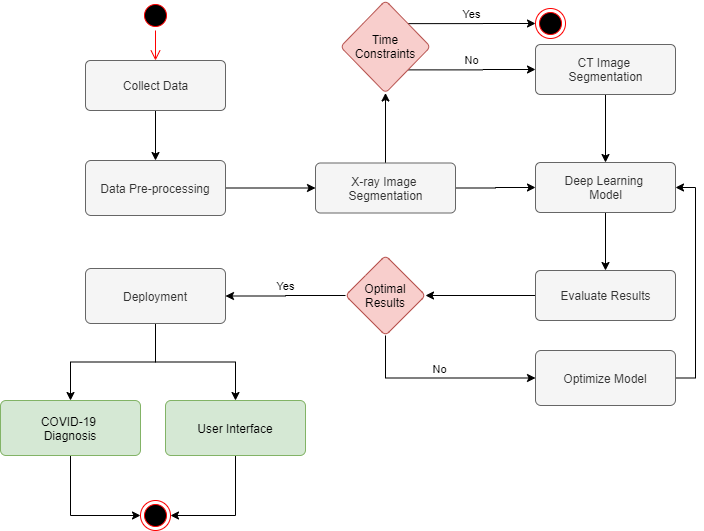
\includegraphics[width=15.5cm]{Images/Implementation Workflow.png}
 \decoRule
 \caption[Implementation Methodology]{Activity Diagram displaying the implementation workflow.}
 \label{fig:Implementation Methodology}
 \end{figure}
 
 \vspace{-2em}
\section{Evaluation Strategy} \label{Evaluation Strategy Section}
Table \ref{tab:Evaluation Strategy} summarizes the methods and strategies used to evaluate each of the Functional Requirements described in Chapter \ref{Requirements Analysis}.

\begin{longtable}{| p{.10\textwidth} | p{.82\textwidth} |} 
\hline
\multicolumn{2}{|c|}{\textbf{Evaluation Strategy}}\\
\hline
\textbf{ID} & \textbf{Description}\\
\hline
FR-1 & \parbox[t]{12.3cm}{\textbf{X-ray Segmentation} \\ The lung segments produced from X-ray scans shall be evaluated based on its capability to identify possible ROIs.}\\\hline
FR-2 & \parbox[t]{12.3cm}{\textbf{CT Segmentation} \\ The lung segments produced from CT scans shall be evaluated based on its capability to identify possible ROIs.}\\\hline
FR-3 & \parbox[t]{12.3cm}{\textbf{COVID-19 Diagnosis using X-ray Scans} \\ The diagnosis results obtained after achieving FR-1 shall be evaluated against various statistical metrics such as Accuracy, Precision and Recall.}\\\hline
FR-4 & \parbox[t]{12.3cm}{\textbf{COVID-19 Diagnosis using CT Scans} \\ The diagnosis results obtained after achieving FR-2 shall be evaluated against various statistical metrics such as Accuracy, Precision and Recall.}\\\hline
FR-5 & \parbox[t]{12.3cm}{\textbf{Visualize Lung Region of Interest's} \\ The ROIs visualized correlates to the observed lung characteristics in COVID-19 patients.} \\\hline
FR-6 & \parbox[t]{12.3cm}{\textbf{Multi-class Diagnosis} \\ The diagnosis results obtained shall be evaluated against various statistical metrics such as Accuracy, Precision and Recall.}\\\hline
FR-7 & \parbox[t]{12.3cm}{\textbf{Web Interface} \\ The user interface developed shall evaluated based on the following metrics, that is, user-friendliness, consistency, familiarity, responsiveness, and intuitiveness\vspace{0.2em}}\\\hline
\caption{Evaluation Strategy}

  \label{tab:Evaluation Strategy}
  \end{longtable}
  
    \vspace{-2em}
\section{Implementation Methodology}
A brief summary of the methodology that would be carried out in semester 2 as well as their evaluation is described in this section.
\subsection{Data Collection}
The two primary sources for collecting open-source anonymized data would be the COVID-19 Kaggle datasets and the scans provided by Cohen et al. \cite{JMD2020} as seen from the literature review. The images obtained shall be separated into X-ray and CT scans separately and furthermore, on the basis of their labels.
\begin{itemize}
    \item \textbf{Testing} - Datasets which correspond to other lung diseases would also be used to analyze the generalizability of the model.
     \item \textbf{Evaluation} - Training would be conducted using  10-fold cross-validation, followed by rigorous verification to prevent the model from either overfitting or underfitting.
\end{itemize}

\subsection{Data Pre-processing}
Before carrying out image segmentation for both X-ray and CT scans, all images in the training dataset shall undergo the same data pre-processing pipeline as per the model's input parameters.
\begin{itemize}
    \item \textbf{Testing} - The model would be tested on images with different dimensions to ensure no input errors are caused.
     \item \textbf{Evaluation} - An input verification technique shall be applied to validate the provided training images before the deep learning workflow commences.
\end{itemize}

\subsection{Image Segmentation}
The provided training images, both X-ray and CT scans shall undergo segmentation such that the ROIs would be highlighted and lead to effective COVID-19 diagnosis
\begin{itemize}
    \item \textbf{Testing} - Multiple image segmentation techniques as suggested by the literature shall be used during the development phase to identify the one that yields the best results.
     \item \textbf{Evaluation} - All models used for experimentation purposes would be documented and the best would be utilized for final demonstration purposes.
\end{itemize}
\subsection{Model Optimization}
As observed in the literature review, multiple studies \cite{CXZ+2020, CYZ+2020, HLR+2020, YHQ+2020, GOM+2020, LLL+2020, CJL+2020, JSB+2020, SFY+2020} indicate variants of the U-Net architecture to be the best suited for CT scan segmentation whereas, for X-rays, variants of ResNet and CNN seem to be ideal as per the research conducted \cite{ZXS+2020, AKP2020, GHT2020, LWA2020}.
\begin{itemize}
    \item \textbf{Testing} - Each of the proposed model variations shall be experimented with for testing purposes, and the results obtained shall be compared to existing literature. 
     \item \textbf{Evaluation} - The results obtained after tweaking the various hyper-parameters for each of the proposed models shall be tracked, thus being able to identify the most optimal set of values.
\end{itemize}


% \section{Research Questions}
% Upon project completion we aim to find answers to the following questions after applying 
% suitable evaluation strategies:

% \begin{itemize}
%   \item Identify whether the ROI's detected by the deep learning model correlates with the lung characteristics observed on COVID-19 patients.
%   \item Compare the results obtained by the deep learning approach with the standard RT-PCR test.
%   \item Feasibility of deploying and utilizing the deep learning model in medical facilities and laboratories for rapid real-time COVID-19 diagnosis.
% \end{itemize}
\chapter{Project Implementation} \label{Project Implementation}

In this section we explore the implementation workflow followed throughout project development phase. This chapter is divided into two main sections, that is, X-rays and CT scans. Within each of these sections, we provide a comprehensive discussion on the approaches and concepts utilized. The implementation workflow ranges from Data Collection to Heatmap Visualization. Before we dive into these sections, we describe our development environment. 

\section{Requirements Analysis}

Our implementation was indeed focused around the Functional Requirements carefully curated during Stage 1 of this project. Most of our requirements revolved around the segmentation and diagnosis of chest X-rays and CT scans, with the former being a mandatory requirement. 

Fortunately, we have been able to experiment with both X-rays and CT scans and successfully build a real-time diagnosis system. Other requirements focused on heatmap generation, multi-class diagnosis, and web interface, which have also been implemented. In addition, we have validated a subset of results obtained with findings observed by a senior Radiologist. 

Our Functional and Non-Functional Requirements generated during Stage 1 along with the Evaluation Strategy can be found in Appendix \ref{Requirements Analysis}.

% We have performed validation of our requirements in Section \ref{reqVal}. 

\section{Development Environment} \label{devEnv}
We have utilized the free-to-use tier of Google Colaboratory to develop our deep learning models. Google provides access to Jupyter Notebooks powered by Tesla K80 GPU with 12 GB RAM and 32 GB disk space. It is also possible for free tier users to access limited number of Tensor Processing Units (TPUs). We have used the latter to enhance performance speed and save processing time.

\section{Source Code}

As mentioned in Section \ref{devEnv}, we have used notebooks provided by Google Colab for developing and evaluating our models. All datasets and notebooks utilized in this project, Flutter code used for our Diagnosis Portal, Python scripts and additional resources are uploaded on our OneDrive repository \footnote{The OneDrive Repository can be found here: \url{https://heriotwatt-my.sharepoint.com/:f:/g/personal/agl2_hw_ac_uk/EmzALshj8olHrfeelAF8h7ABPoVhQBsnViMaiNgTp9Zc6g?e=FbzZhj}}. We have also uploaded the Source Code on GitHub as per the requirements \footnote{GitHub Repository can be found here: \url{https://github.com/AlisterLuiz/Dissertation}}. We have also deployed our Diagnosis Portal that allows real-time COVID-19 Diagnosis \footnote{Link to the Diagnosis Portal: \url{http://40.76.124.61/}}.


\section{X-ray Scans}
The following section illustrates the workflow utilized to collect data, develop and test our deep learning models. We also demonstrate various concepts used to improve model performance.

\subsection{Data Collection}

Our model was trained and tested using images from a Kaggle dataset\footnote{Available at: \url{https://www.kaggle.com/prashant268/chest-xray-covid19-pneumonia}}. The dataset is compiled from multiple  sources \cite{GAN2020, MOO2018, AGC2020}. It is an open-source database of COVID-19 cases which includes X-ray scans. It includes COVID-19 and Pneumonia cases as well as Healthy Chest Scans.


Furthermore, given the objective of our classification task to identify COVID-19 patterns, only the posterior-anterior view of the lungs was considered for training and testing. This view visualizes the bony thoracic cavity, mediastinum, and great vessels \cite{MUR2020}. This choice allowed us to reduce the number of training instances and work with a less unbalanced dataset. 

\subsection{Data Pre-processing}

As we successfully identified a suitable dataset and collected the required X-ray scans, it was now time to pre-process the data and prepare it for model training purposes. This section highlights all the pre-processing procedures we have carried out.

\subsubsection{Data Augmentation} \label{aug}

To generate more training samples and reliable training results we have performed Data Augmentation. It was indeed necessary to balance the dataset before augmenting our scans. 

In each fold of the 10-fold cross validation, we take 10\% of dataset out to be used as validation dataset. The remaining 90\% undergoes an augmentation step. The augmentation step uses three operators to produce slightly modified image, namely rotation, zooming and shearing. Image rotation rotates image by $5^{\circ}$. Zooming applies a +2\% zoom. Shearing distorts an image along an axis (essentially converting rectangles into parallelograms), applies a $2^{\circ}$ counter-clockwise distortion. 

To perform augmentation with these three operators we have utilized Keras' Image Data Generator class which generates batches of tensor image data with real-time data augmentation \cite{KER}. Given memory limits of Google Colab, we have generated 600 images per class using training data which was appended to our existing dataset. Therefore, augmented training data was fed into our deep learning model for training. A summary of our dataset is provided in Section \ref{eda}.

\subsubsection{Exploratory Data Analysis} \label{eda}
As an initial insight into our dataset, we have plotted the number of X-ray scans per class before and after we have balanced the dataset, these figures are plotted in Figure \ref{fig:dataset_dist}. From our initial data collection, we received 575 COVID-19, 4273 Pneumonia, and 2583 healthy chest scans. After balancing, our dataset comprised of 572 scans from each class respectively.

% \vspace{1em}

\begin{figure}[H]
        \begin{subfigure}[b]{0.5\textwidth}
                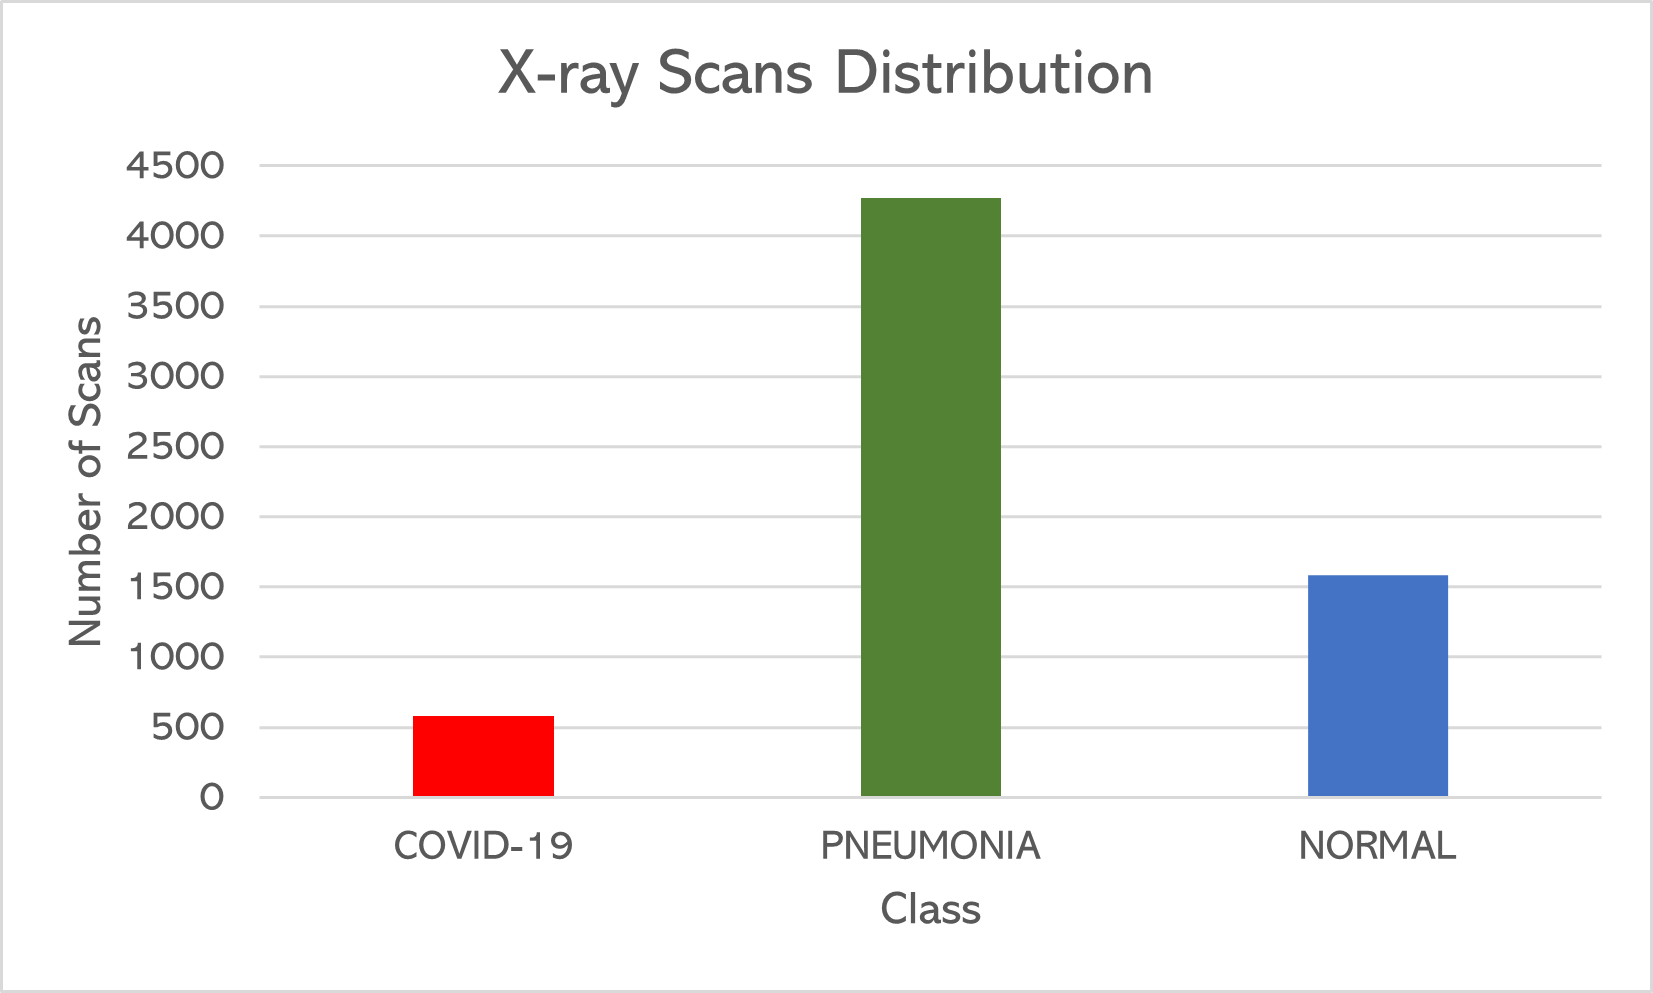
\includegraphics[width=\linewidth]{Images/DatasetDistribution.png}
                \caption{Unbalanced Dataset}
                \label{fig:unbalanced}
        \end{subfigure}%
        \begin{subfigure}[b]{0.5\textwidth}
                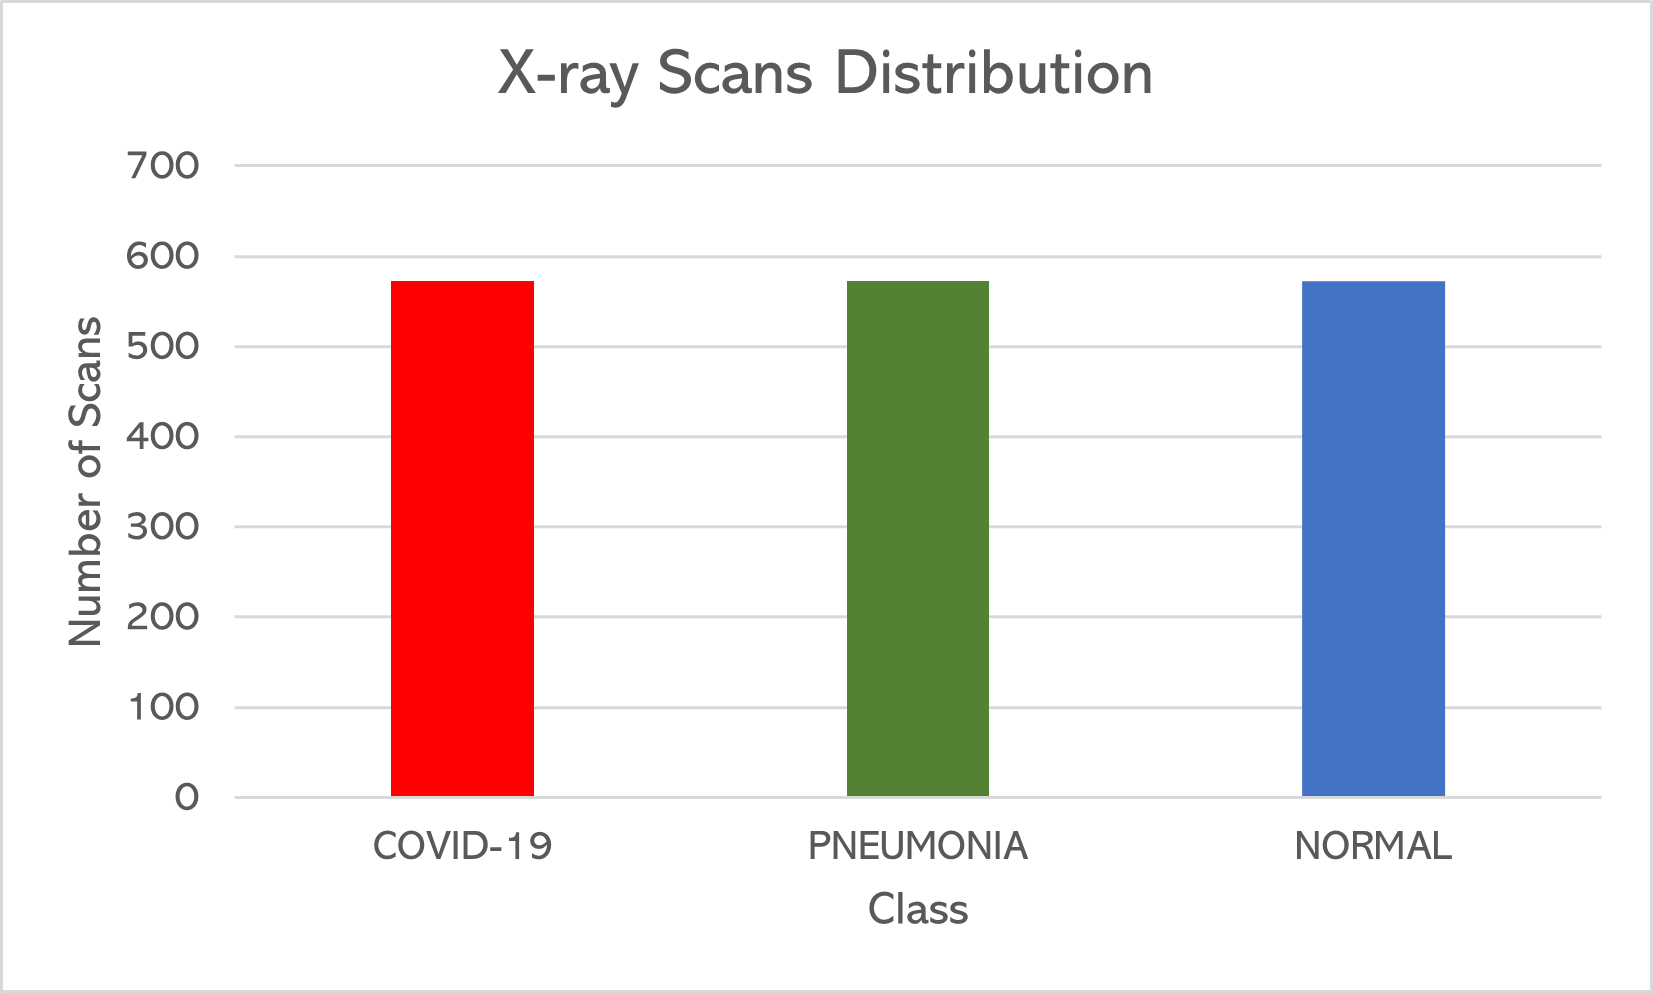
\includegraphics[width=\linewidth]{Images/DatasetDistribution2.png}
                \caption{Balanced Dataset}
                \label{fig:balanced}
        \end{subfigure}%
        %\\\centering
            %\decoRule
        \caption{Dataset Distribution for X-ray Scans}\label{fig:dataset_dist}
\end{figure}
\vspace{-1em}
Post augmentation we have been able to yield more scans per class to further enhance the generalizability of classification. Table \ref{tab:Dataset Info} provides a detailed overview before and after augmentation. Figure \ref{fig:xray data} contains sample X-ray scans from our dataset along with their corresponding labels.

\begin{longtable}{| p{.13\textwidth} | p{.06\textwidth} | p{.18\textwidth} | p{.15\textwidth} | p{.18\textwidth} | p{.11\textwidth} |} 

    \hline
\textbf{Disease} & \textbf{Total}    & \textbf{Non-augmented Training}   &\textbf{Augmented Training} \\
\hline
			COVID-19    &572   &468    &1070
\\\hline
			Pneumonia   &572   &468    &1070
\\\hline
			Normal      &572   &468    &1070
\\\hline 

\caption{Training Dataset Post Augmentation}

  \label{tab:Dataset Info}
    \end{longtable}

\begin{figure}[H]
	\centering
	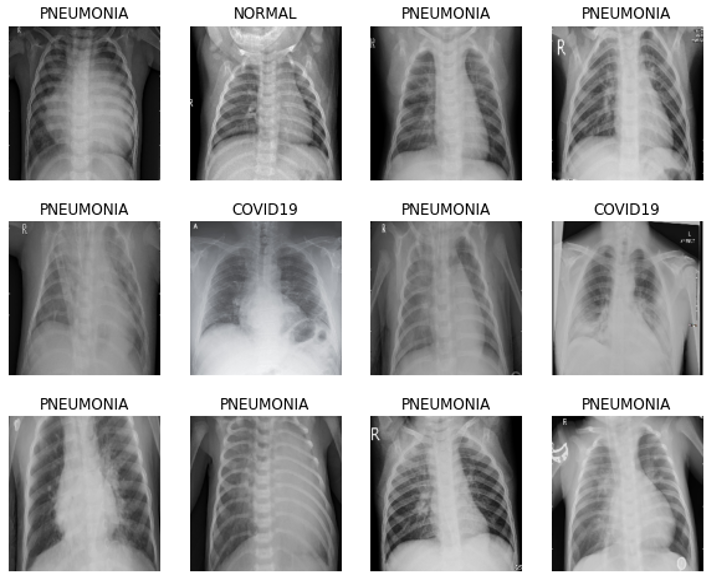
\includegraphics[width=12cm, height=8.5cm]{Images/SampleScans.png}
	
            %\decoRule
	\caption{\small Sample of X-ray scans with labels for model training.}
	\label{fig:xray data}
\end{figure}

\subsection{Methodology}

As we have now explored our dataset, we present the methodology used to construct and develop our deep learning models.  


\subsubsection{Proposed Models}

We have constructed, developed, and evaluated three pre-trained base models on the ImageNet dataset \cite{IMG}, that is, DenseNet121, ResNet50, and VGG16. Each of these base models were trained on the augmented dataset, and ensembled to further improve classification performance. The model architectures for each of these three models are provided in Figure \ref{fig:arch}.

Each of the pre-trained models we have experimented with has their own set of advantages. Dense-Net's are known to ease vanishing-gradient problem, reinforce feature propagation, promote feature reuse, and reduce the number of training parameters \cite{HLW+2016}.

Residual Networks are known for their faster training speeds and powerful representational ability \cite{BAK2016, FEN2017}. Furthermore, from Literature Review (Section \ref{LR}) we observe that ResNet variants seem to be a popular choice among studies performing image classification.
\vspace{0.5em}
\begin{figure}[H]
        \begin{subfigure}[]{0.49\linewidth}
                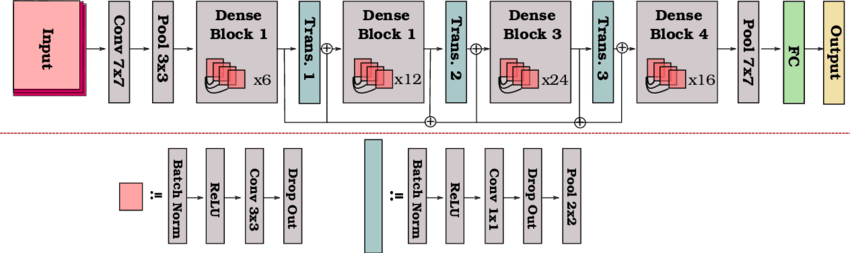
\includegraphics[height=3cm]{Images/DenseNet121.png}
                \caption{DenseNet121 \cite{DEN}}
                \label{fig:DenseNet}
        \end{subfigure}%
        \begin{subfigure}[]{0.49\linewidth}
                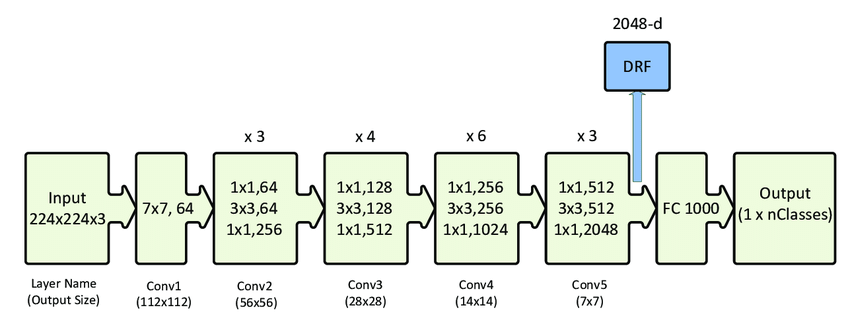
\includegraphics[height=3cm]{Images/ResNet.png}
                \caption{ResNet50 \cite{MOB+2020}}
                \label{fig:ResNet}
        \end{subfigure}%

\end{figure}

\begin{figure}[H]\ContinuedFloat
          \begin{center}
        \begin{subfigure}[]{0.7\linewidth}
                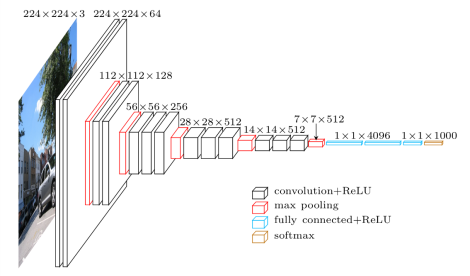
\includegraphics[height=6cm, width=\linewidth]{Images/VGG16.png}
                \caption{VGG16 \cite{VGG}}
                \label{fig:VGG}
        \end{subfigure}%
    
        \end{center}
        %\\\centering
            %\decoRule
        \caption{X-ray Model Architectures}\label{fig:arch}


\end{figure}
\vspace{-2em}
VGG is the simplest model among the three and is usually used for benchmarking \cite{SKZ2015}. Built as a deep CNN, VGG outperforms baselines on many tasks and datasets outside of ImageNet \cite{WJY2019}.

These pre-trained models were readily available on the Keras applications library \cite{KAP}. We have used these pre-trained models as a starting point to build our classification models.

\vspace{1em}

\begin{lstlisting}
pretrainedDenseNet = tf.keras.applications.DenseNet121(input_shape = (imageSize, imageSize, 3), weights = 'imagenet', include_top = False)

pretrainedResNet = tf.keras.applications.ResNet50(input_shape = (imageSize, imageSize, 3), weights = 'imagenet', include_top = False)
pretrainedVGG = tf.keras.applications.VGG16(input_shape = (imageSize, imageSize, 3), weights = 'imagenet', include_top = False)
\end{lstlisting}



\subsubsection{Keras Callbacks} \label{KCXray}

The Keras Callbacks API is an effective utility which aids in enhancing model training. A callback is an object that can perform actions at various stages of training, usually in between epochs or when training begins or ends \cite{KCB}. For training our deep learning models on X-ray scans we utilized three Callback functions, that is, EarlyStopping, ReduceLROnPlateau, and ModelCheckpoint.

EarlyStopping (ES) ends training when a monitored metric has stopped improving \cite{KES}. For each of our deep learning models we have used the ES Callback with the following parameters. 

\vspace{1em}
\begin{lstlisting}
esCallback = tf.keras.callbacks.EarlyStopping(monitor='val_loss', patience=15, verbose=1)
\end{lstlisting}

We monitor validation loss and terminate our training as soon as model converges. An added benefit of using this callback is reduced processing time required to train our deep learning models.

The next callback, ReduceLROnPlateau reduces the learning rate when a metric has stopped improving, in our case validation loss. This callback proved to be fruitful while training our deep learning models. Reducing the Learning Rate by a factor of 0.5, helped the models to converge faster and overcome learning plateaus \cite{KLR}. 
\vspace{1em}
\begin{lstlisting}
lrReduce = tf.keras.callbacks.ReduceLROnPlateau(monitor='val_loss', factor=0.5, min_delta=0.0001, patience=8, verbose=1)
\end{lstlisting}

ModelCheckpoint, simply saves the best performing model during training depending on the given parameter \cite{KMC}.
\vspace{1em}

\begin{lstlisting}
mcpSave = ModelCheckpoint('Path to Save Model', save_best_only=True, monitor='val_loss', mode='min')
\end{lstlisting}

Utilizing each of our these three callbacks allowed us to increase the efficiency and performance of our models.

\subsubsection{Transfer Learning} \label{tl}
Transfer learning is a machine-learning technique where a model trained for an application with some dataset is re-used on another dataset. The pre-trained model approach to transfer learning consists of using the source model as a starting point for training the target model. 

In order to reduce training time and improve accuracy, we adopted the pre-trained transfer learning approach. We have used a model trained with large volume of images from the ImageNet dataset for classification tasks \cite{IMG}. Using the pre-trained model, we trained only the final layer so as to alter its weights to suit our dataset. All other layers used fixed weights obtained from the prior training using the ImageNet dataset. A very simple illustration of the Transfer Learning approach is shown in Figure \ref{fig:transfer learning}. 


\begin{figure}[htbp]
	\centering
	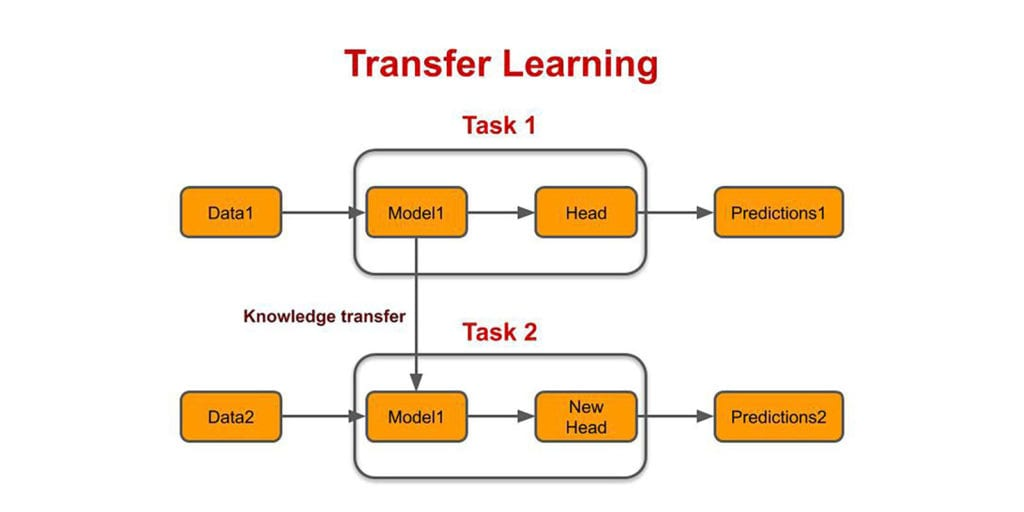
\includegraphics[width=15cm]{Images/Transfer Learning.jpg}
	    %\decoRule
	\caption{\small A simple representation of Transfer Learning Technique \cite{TBT2019}}
	\label{fig:transfer learning}
\end{figure}

\subsubsection{Ensemble Learning} \label{elx}

Given our base models, an ideal approach to improve upon the classification performance was to implement Ensemble Learning. Ensemble Learning involves combining several classifiers to solve a particular problem. The combined model generally achieves optimum predictive performance when compared to any of the constituent learning algorithms alone \cite{POL2019, LUT2017}.

Our approach involves utilizing the best performing model after cross-validation from each of the three base models. We take the last dense layer of each model, that is, without the heads, and provide the network an opportunity to learn from these dense layers before applying the softmax function. Indeed, we have frozen the layer weights of our base models, before ensembling. 

Keras' Concatenate layer \cite{CON} allows us easily merge or stack these dense layers and yield the final prediction after applying the softmax activation. As expected, we have observed an increase in classification performance through ensembling our base models. An illustration of the same is provided in Figure \ref{fig:ensemble learning}.

\begin{figure}[H]
	\centering
	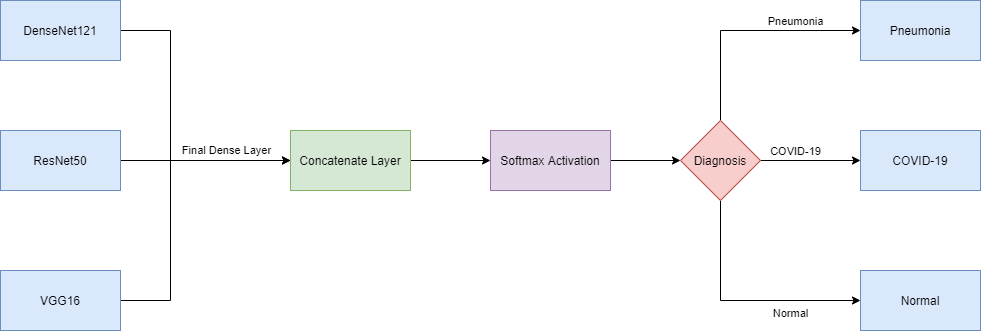
\includegraphics[width=15.5cm]{Images/Ensemble.png}
	    %\decoRule
	\caption{\small Ensemble Learning Illustration for X-ray Scans}
	\label{fig:ensemble learning}
\end{figure}


\subsubsection{Model Training}

We have used 10-fold cross validation and leave an eleventh fold to test the 10 models on it as unseen data. Indeed, 10-fold cross validation produces 10 models that, collectively, saw all the training dataset. We have seen our dataset distribution is Section \ref{eda}. We built a balanced dataset of 572 samples of each of the classes (572 is a multiple of 11). The size of the eleventh fold, to which we refer to from now on as \textit{unseen data}, is 52. 

\begin{longtable}{| p{.13\textwidth} | p{.06\textwidth} | p{.18\textwidth} | p{.15\textwidth} | p{.18\textwidth} | p{.11\textwidth} |} 

    \hline
\textbf{Disease} & \textbf{Total}    & \textbf{Non-augmented Training}   &\textbf{Augmented Training} &\textbf{Non-augmented Testing} & \textbf{Unseen Data} \\
\hline
			COVID-19    &572   &468    &1070   &52   &52
\\\hline
			Pneumonia   &572   &468    &1070   &52   &52
\\\hline
			Normal      &572   &468    &1070   &52   &52
\\\hline 

\caption{Dataset Distribution}

  \label{tab:Dataset Info}
    \end{longtable}
\vspace{-1em}
At each of the 10 iterations of 10-fold cross validation, we take 10\% of the dataset out to be used for testing. The remaining 90\% undergoes the augmentation steps as mentioned in Section \ref{aug}. 

The augmentation of each of the 468 samples of each class (90\% of 520) resulted in creating 1070 samples per class. Since we have three classes, COVID-19, Pneumonia and Normal, the total number of samples in the final training dataset is of 3,210. Only the training dataset was augmented; no augmentation was applied to the test dataset. Table \ref{tab:Dataset Info} shows the size of the data we used. 

We trained our models for 50 epochs with a batch size of 210 per forward/backward pass. We have also initialized all the callbacks mentioned in Section \ref{KCXray}. Post training, the results were evaluated using scikit-learns classification report function \cite{SCR}. A confusion matrix was also displayed after every epoch indicating the model performance \cite{SCM}, which also allows us to extract useful metrics and determine the best performing model. A sample snippet of code which calls the fit function is provided below.

\vspace{1em}
\begin{lstlisting}
history = model.fit(augmentedDataX, YCatAug, validation_data = (XTrain[test], YCatVal), callbacks=[lrReduce, esCallback, mcpSaveDenseNet], epochs=50, batch_size=210)
\end{lstlisting}

\subsubsection{Heatmap Visualization}

For the purpose of building a more interepretable model, we generated heatmaps for the provided X-ray scans. The heatmaps highlight the regions that led to the classification by our model. We calculated the Grad-CAM heatmaps with the help of Keras' Computer Vision examples \cite{KCV}. The same Grad-CAM class activation visualization example provided by François Chollet was utilized in our implementation \cite{KGM}. We have generated Grad-CAM heatmaps from each of our three base models. We have utilized Numpy \cite{NUM} to average obtained heatmaps and produce the final consolidated heatmap.

Grad-CAM heatmaps highlight regions in the lungs which, as discussed in section \ref{Interpreting Deep Learning Results}, exhibit the most common characteristics in patients diagnosed with COVID-19. These include features such as GGO’s, consolidations, lesions, and crazy-paving patterns, which are some of the most contributing features to diagnosis. This technique provides interpretation means that would assist radiologists in identifying the same lung characteristics as with traditional segmentation-based methods. Regions in red are the most influential in making the decision, whereas blue regions are the least influential.


\subsubsection{Workflow Summary Illustration}

\begin{figure}[H]
	\centering
	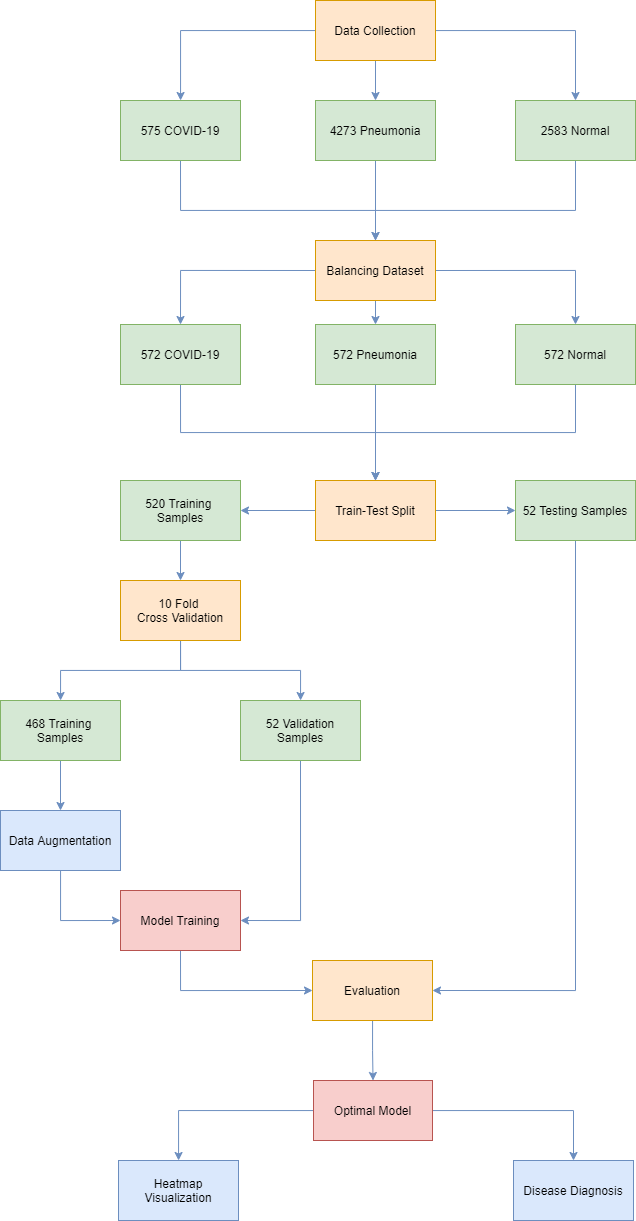
\includegraphics[width=13cm, height= 22.5cm]{Images/X-ray Workflow.png}
	    %\decoRule
	\caption{\small X-ray Workflow Illustration}
	\label{fig:Xray Illustration}
\end{figure}

\section{CT Scans}
The following section explores the second part of our project, that is, CT scans. A similar workflow has been utilized for CT classification purposes with minor changes in between such as Lung Parenchyma extraction as an additional pre-processing step.

\subsection{Data Collection}

We have used an open-source Kaggle CT dataset \footnote{Available at \url{https://www.kaggle.com/azaemon/preprocessed-ct-scans-for-covid19}} for training and testing our models. All the images present in this dataset was collected by the authors from the Frontier Exploration Program of Huazhong University of Science and Technology, the program for HUST Academic Frontier Youth Team, and the Fundamental Research Funds for the Central Universities \cite{JCY+2020, ICT2019}. 

This dataset is comprised of two parts, the original and pre-processed CT scans of COVID-19 and Normal patients readily available for model training purposes. The code to pre-process the original CT scans was given by the author of this dataset. Applying them we were able to extract the lung parenchyma, which proved to be a vital pre-requisite to train CT data.

\subsection{Data Pre-processing}

In the following subsections, we provide a brief overview on the various Data Pre-processing techniques we have applied. 
\subsubsection{Lung Parenchyma Extraction}

Even though the Kaggle dataset already contains the pre-processed dataset, it was necessary for us to understand the process involved in extracting the lung parenchyma, so as to do the same for incoming unseen samples in a real-time application.

This process for extracting the lung parenchyma was as per the suggestions by Ning et al. \cite{ICT2019}. The source code involved a fill water function that applied certain filter masks to further fine tune the extracted lung parenchymas. An example of a CT scan image before and after extracting lung parenchyma is displayed in Figure \ref{fig:extract}. Indeed, the processed CT images were used for model training and evaluation purposes.

\begin{figure}[H]
        \begin{subfigure}[b]{0.5\textwidth}
                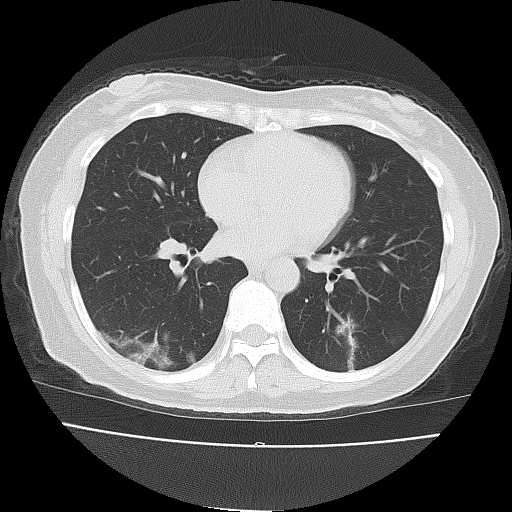
\includegraphics[width=\linewidth]{Images/NonProcessed pCT1.jpg}
                \caption{Original CT Scan}
                \label{fig:unbalanced}
        \end{subfigure}%
        \begin{subfigure}[b]{0.5\textwidth}
                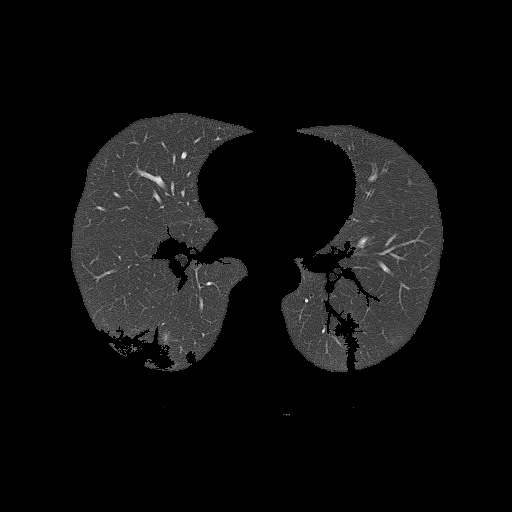
\includegraphics[width=\linewidth]{Images/Processed pCT1.jpg}
                \caption{Processed CT Scan}
                \label{fig:balanced}
        \end{subfigure}%
        %\\\centering
            %\decoRule
        \caption{Lung Parenchyma Extraction}\label{fig:extract}
\end{figure}

\subsubsection{Data Augmentation}

Similar to our X-ray pre-processing workflow we have augmented the CT data so as to improve the reliability of our model prediction and handle unpredictabilities of real-world data. The same augmentation parameters were applied at each of the 10 iterations of 10-fold cross validation, that is, $5^{\circ}$ rotation, +2\% zooming, and $2^{\circ}$ shearing. Keras' Image Data Generator class was once again utilized for performing real-time data augmentation \cite{KER}. Once again prioritizing the limits of Google Colab, we have generated 2000 augmented images per class and is appended to the existing dataset.

\subsubsection{Exploratory Data Analysis} \label{EDA CT}

To familiarize ourselves with the data, the first step was to plot the number of CT scans per class. Similar to X-ray scans, the plots include the counts before and after balancing the dataset. The plots are displayed in Figure \ref{fig:CTdist}. The number of training scans post augmentation is tabulated in Table \ref{tab:Dataset Info CT}. After collecting data from the Kaggle Dataset we have ended up 4001 COVID-19 and 9979 Normal scans. After balancing our dataset we have ended up with 3993 scans per class.

\begin{figure}[H]
        \begin{subfigure}[b]{0.5\textwidth}
                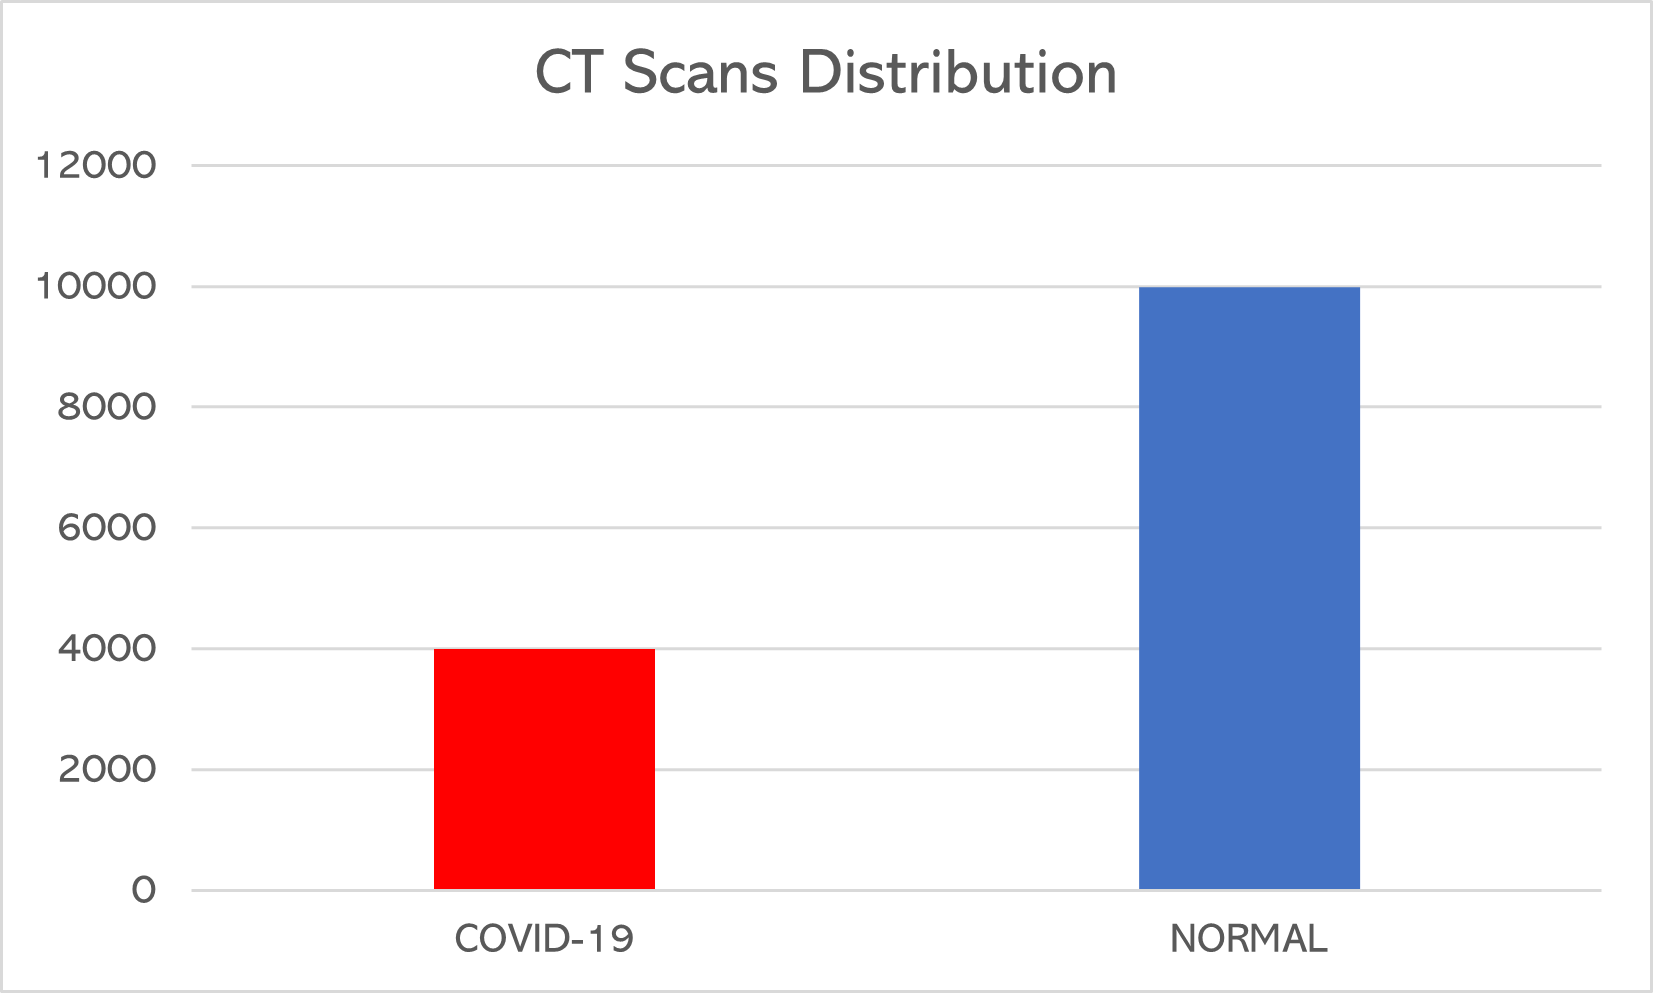
\includegraphics[width=\linewidth]{Images/CTDistribution.png}
                \caption{Unbalanced Dataset}
                \label{fig:unbalanced}
        \end{subfigure}%
        \begin{subfigure}[b]{0.5\textwidth}
                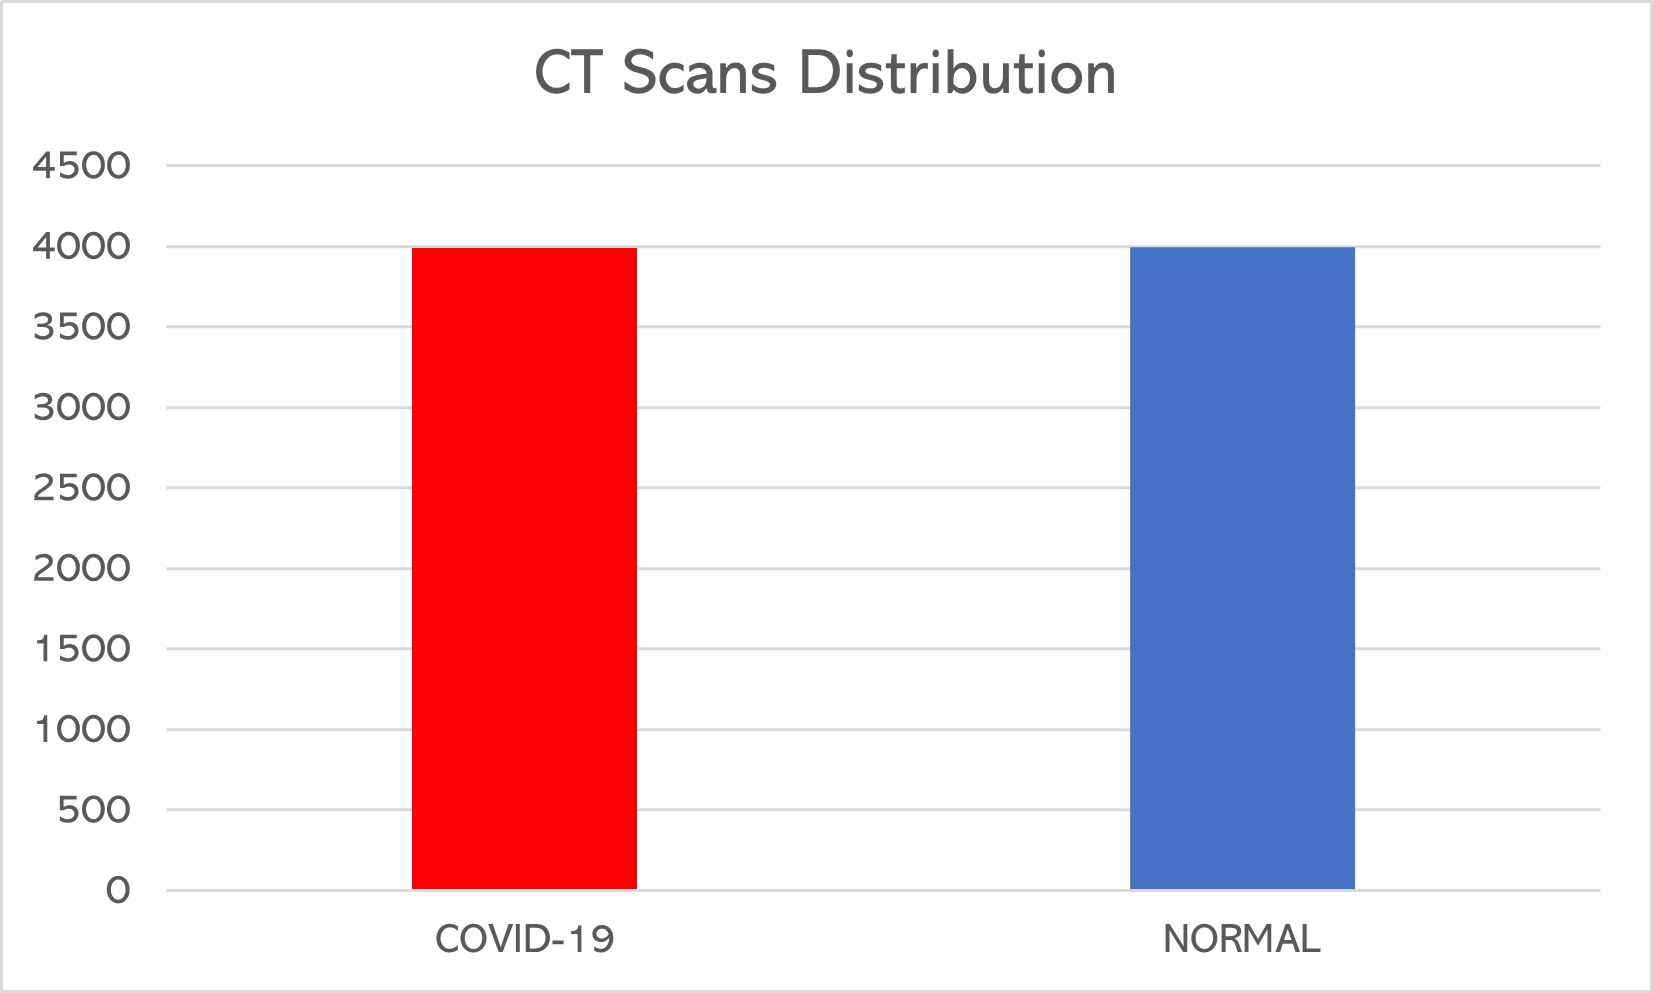
\includegraphics[width=\linewidth]{Images/CTDistribution2.png}
                \caption{Balanced Dataset}
                \label{fig:balanced}
        \end{subfigure}%
        %\\\centering
            %\decoRule
        \caption{Dataset Distribution}\label{fig:CTdist}
\end{figure}

\begin{longtable}{| p{.13\textwidth} | p{.06\textwidth} | p{.18\textwidth} | p{.15\textwidth} | p{.18\textwidth} | p{.11\textwidth} |} 

    \hline
\textbf{Disease} & \textbf{Total}    & \textbf{Non-augmented Training}   &\textbf{Augmented Training} \\
\hline
			COVID-19    &3993   &3267    &5270
\\\hline
			Normal      &3993   &3267    &5270
\\\hline 

\caption{Training Dataset Post Augmentation}

  \label{tab:Dataset Info CT}
    \end{longtable}

We have also displayed a subset of our CT scans dataset along with their labels in Figure \ref{fig:ct data}.


\begin{figure}[H]
	\centering
	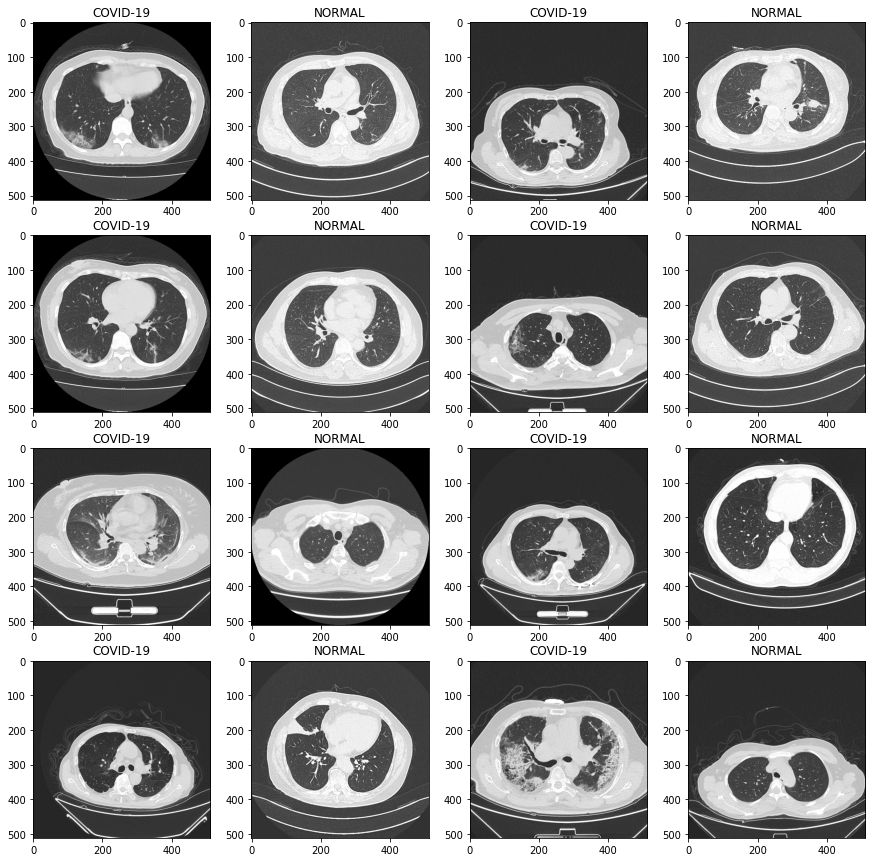
\includegraphics[width=10.5cm, height=10.5cm]{Images/CTScansDist.png}
            %\decoRule
	\caption{\small Sample of unprocessed CT scans with labels for model training.}
	\label{fig:ct data}
\end{figure}

\subsection{Methodology}

Our proposed methodology for CT scans is similar to that of X-ray's to keep our workflow consistent. There are indeed changes in our proposed models and certain parameter values. The following sections elaborates on these differences. 
\subsubsection{Proposed Models}

For CT Scans we have experimented with three models, that is, UNet, UNet++, and Attention UNet. These variants of the base UNet model seems to be popular among literature. The UNet++ and Attention UNet models were Ensembled to improve the classification performance, similar to our X-ray diagnosis workflow. Each of these three model architectures are provided in Figure \ref{fig:ctmodels}.

The UNet model was originally created for Bio-medical Image Segmentation purposes \cite{RFT2015}. As its name indicates, the architecture consists of a 'U' structure, as shown in Figure \ref{fig:unet}. The basic idea revolves around the notion that the same feature maps used for image contraction is utilized to expand a vector to a segmented image. This would help in preserving the structural integrity of the image and greatly reduce image distortion \cite{HSA2018}. The UNet architecture is comprised of three sections, which are, contraction, bottleneck, and expansion respectively.

\begin{figure}[H]
        \begin{subfigure}[b]{0.5\textwidth}
                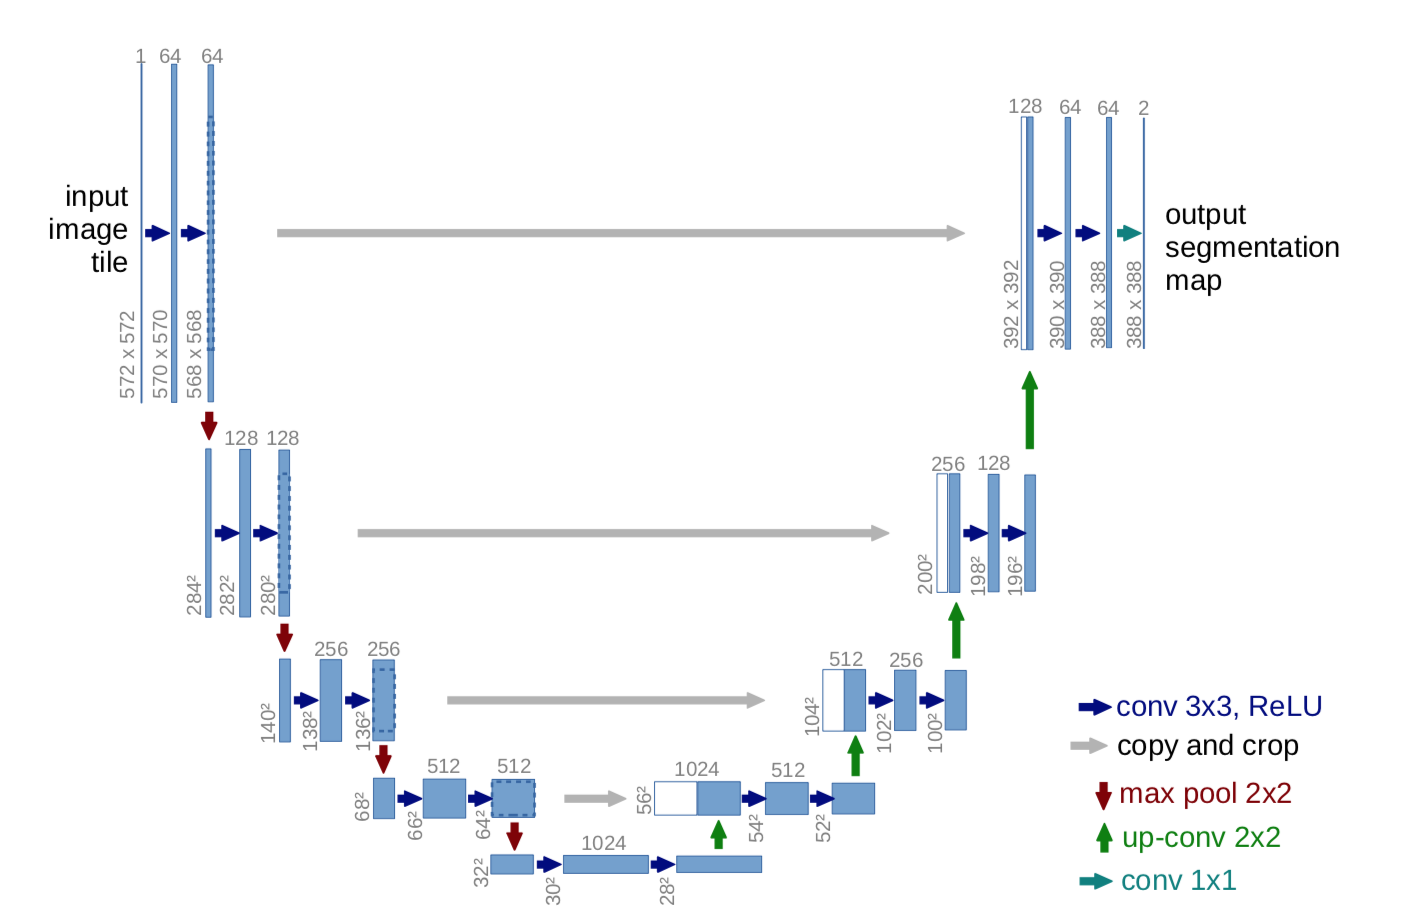
\includegraphics[height=4cm]{Images/UNet.png}
                \caption{UNet \cite{UNT}}
                \label{fig:unet}
        \end{subfigure}%
        \begin{subfigure}[b]{0.5\textwidth}
                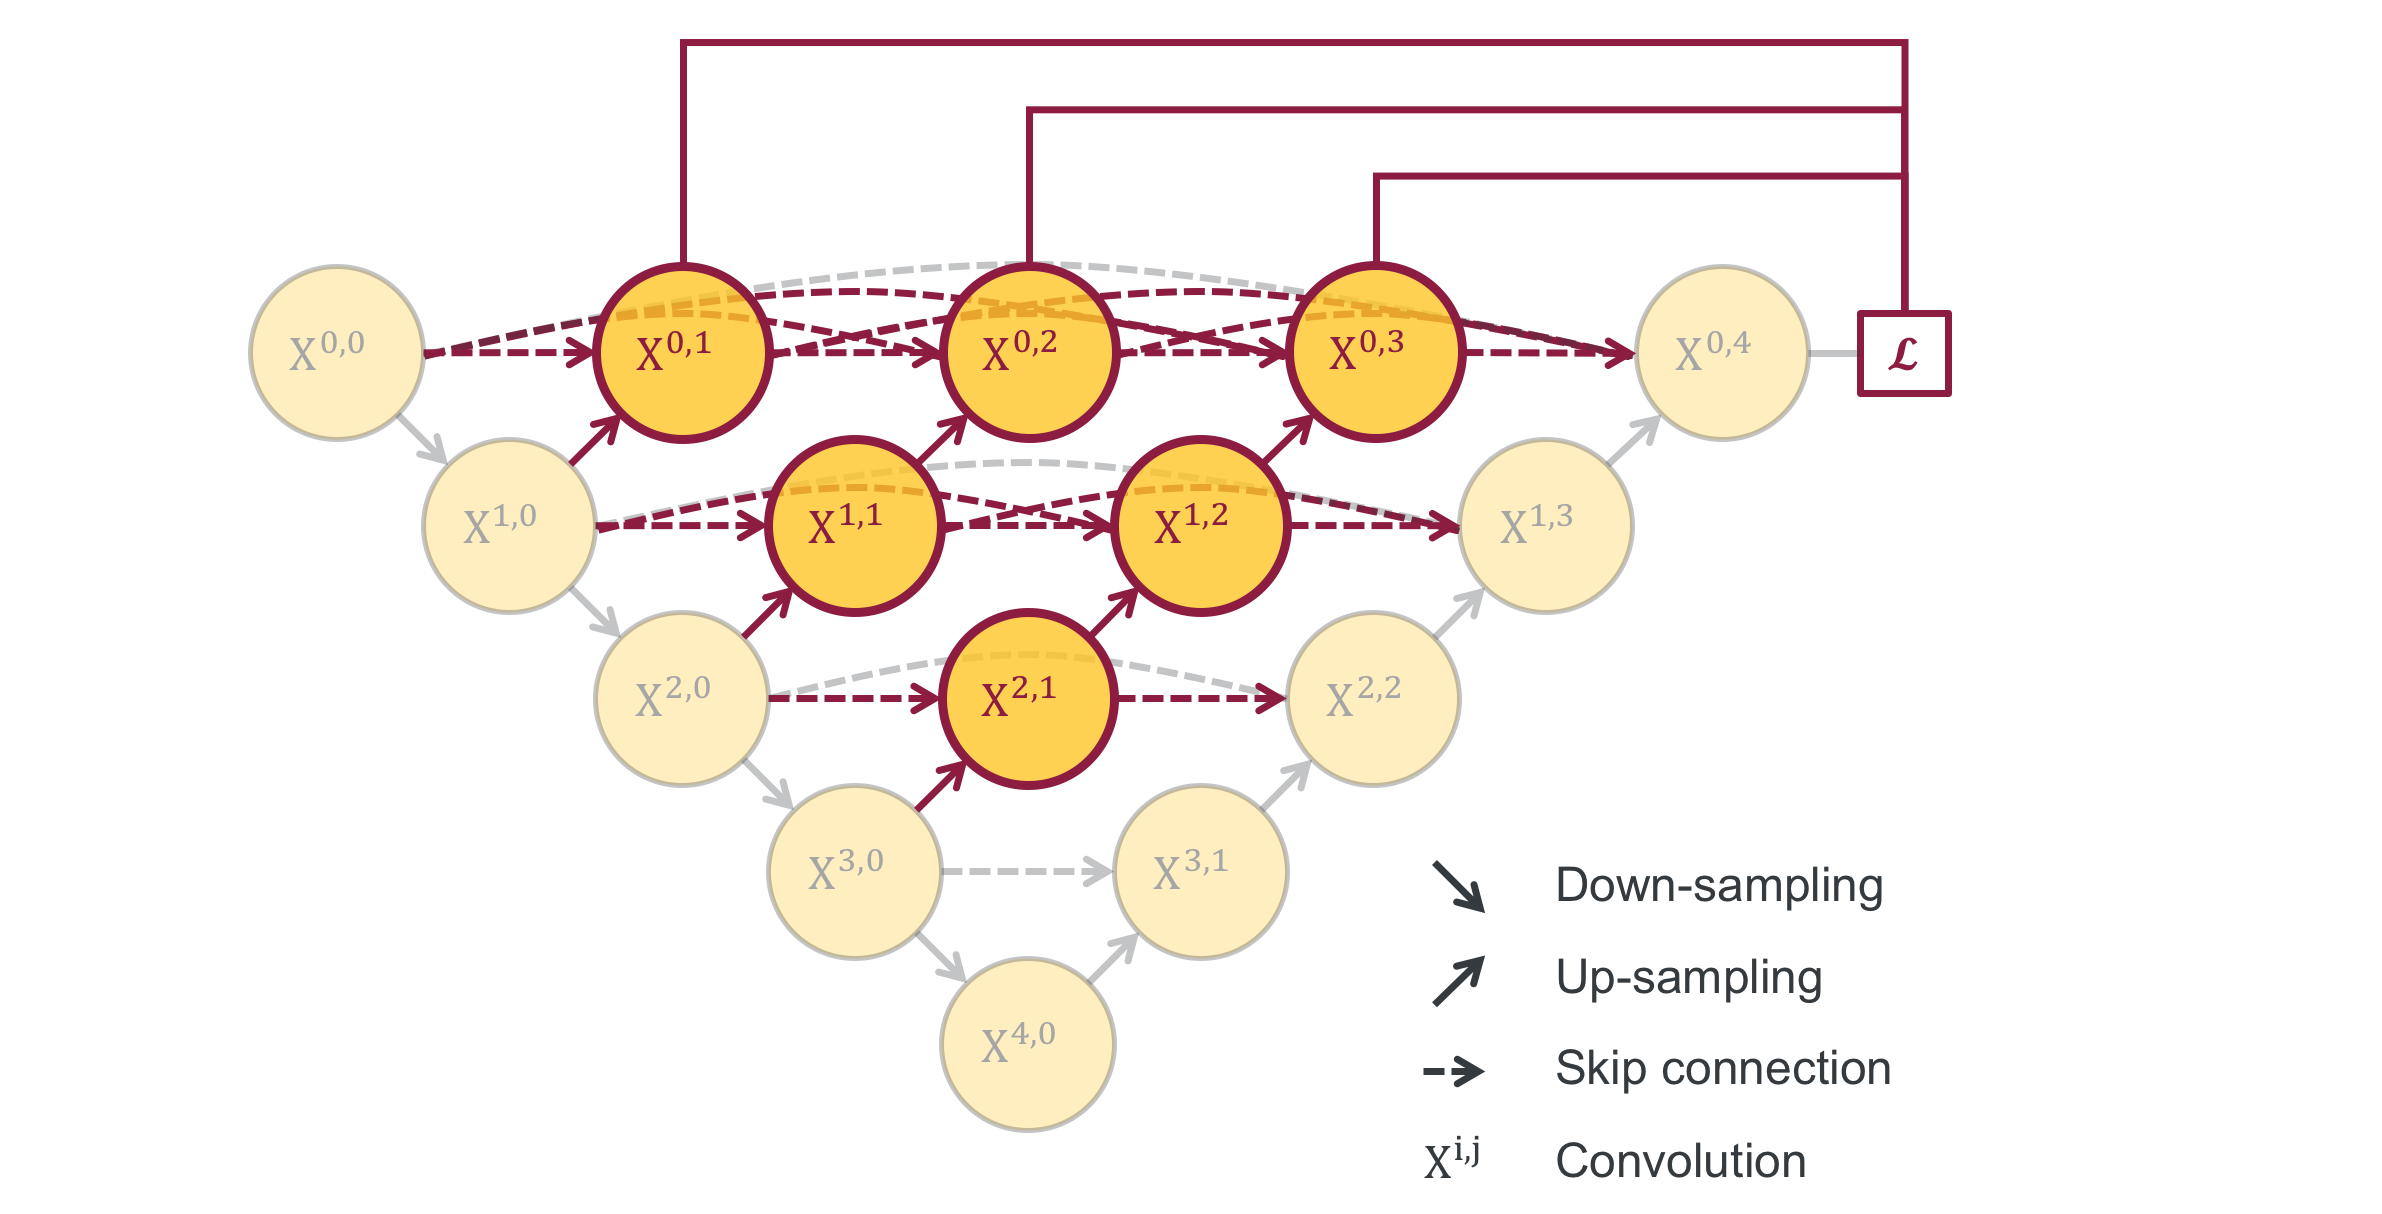
\includegraphics[height=4cm]{Images/UNet++.png}
                \caption{UNet++ \cite{UNT+}}
                \label{fig:unet++}
        \end{subfigure}\\\\
        \begin{center}
         \begin{subfigure}[b]{0.5\textwidth}
                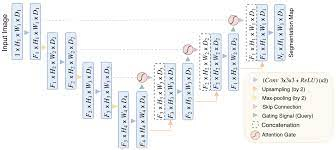
\includegraphics[width=\linewidth]{Images/Att UNet.jpg}
                \caption{Attention UNet \cite{AUN}}
                \label{fig:attUnet}
        \end{subfigure}%
        %\\\centering
            %\decoRule
        \caption{CT Model Architectures}\label{fig:ctmodels}
        \end{center}
\end{figure}

UNet++ is another powerful architecture for medical image segmentation \cite{ZSM+2020}. UNet++ has three major additions when compared to the original UNet model proposed by Ronneberger, that is, redesigned skip pathways, dense skip connections, and deep supervision \cite{JHJ2019}. One caveat of using the UNet++ due to these additions is that the training time is almost doubled when compared to a simple UNet.

Attention UNet aims to only highlight the relevant activations during training, thus significantly reducing computation time. This is made possible using attention gates which uses additive soft attention. As its name suggests, the name pays attention or focuses on certain parts of the provided image \cite{VIN2020, OSF+2020}. When compared to a UNet model, the computation time is only slightly longer. The code snippets initializing each of the three models have been provided below.

\vspace{1em}
\begin{lstlisting}
pretrainedUNet = kerasModels.unet_2d((imageSize, imageSize, 3), filter_num=[64, 128, 256, 512, 1024], n_labels=2, stack_num_down=2, stack_num_up=2, activation='ReLU', output_activation='Sigmoid', batch_norm=True, pool=False, unpool=False, backbone='ResNet50V2', weights='imagenet', freeze_backbone=True, freeze_batch_norm=True, name='unet') 

pretrainedUNetPlus = kerasModels.unet_plus_2d((imageSize, imageSize, 3), filter_num=[64, 128, 256, 512, 1024], n_labels=2, stack_num_down=2, stack_num_up=2, activation='ReLU', output_activation='Sigmoid', batch_norm=True, pool=False, unpool=False, backbone='ResNet50V2', weights='imagenet', freeze_backbone=True, freeze_batch_norm=True, name='unetplus')

pretrainedAttUNet = kerasModels.att_unet_2d((imageSize, imageSize, 3), filter_num=[64, 128, 256, 512, 1024], n_labels=2, stack_num_down=2, stack_num_up=2, activation='ReLU', atten_activation='ReLU', attention='add', output_activation='Sigmoid', batch_norm=True, pool=False, unpool=False, backbone='ResNet50V2', weights='imagenet', freeze_backbone=True, freeze_batch_norm=True,  name='attunet') 
\end{lstlisting}

\subsubsection{Keras Callbacks}

We have utilized the same set of callbacks as we have used for our X-ray models, that is, EarlyStopping, ReduceLROnPlateau, and ModelCheckpoint. However, there have been differences in the parameters especially for EarlyStopping as the UNet models tend to stop training before reaching convergence. Therefore, it was necessary for us to increase the patience parameter depending the variant of UNet model. The following code snippets showcase the parameters used for EarlyStopping Keras callback.

\vspace{1em}
\begin{lstlisting}
UNetESCallback = tf.keras.callbacks.EarlyStopping(monitor='val_loss', patience=80, verbose=1)
AttUNetESCallback = tf.keras.callbacks.EarlyStopping(monitor='val_loss', patience=80, verbose=1)
UNetPlusESCallback = tf.keras.callbacks.EarlyStopping(monitor='val_loss', patience=140, verbose=1)
\end{lstlisting}

Furthermore, for the UNet++ model we have provided custom parameters for the ReduceLROnPlateau callback to achieve optimal convergence and thereby increase classification accuracy.

\vspace{1em}
\begin{lstlisting}
UNetPluslrReduce = tf.keras.callbacks.ReduceLROnPlateau(monitor='val_loss', factor=0.5, min_delta=0.0001, patience=16, verbose=1)
\end{lstlisting}

\subsubsection{Transfer Learning}

We have applied the Transfer Learning technique for CT scan classification as well to avail its benefits such has reduced training time and improvement in accuracy as discussed in Section \ref{tl}. The only difference from our X-ray scan implementation is that we have used a different Python package, Keras UNet Collection \cite{KUC}, which contains pre-trained UNet model and its variants on the large ImageNet dataset \cite{IMG}. 

This package allowed us to easily access different UNet variants and contains various tweakable parameters allowing us to customize or fine-tune our models for training and evaluation purposes. From the code snippet we can clearly see the weights parameter which initializes the model with ImageNet weights. Similar to our X-ray implementation, we have only set the final layer to be trainable.

\vspace{1em}
\begin{lstlisting}
pretrainedUNet = kerasModels.unet_2d((imageSize, imageSize, 3), filter_num=[64, 128, 256, 512, 1024], n_labels=2, stack_num_down=2, stack_num_up=2, activation='ReLU', output_activation='Sigmoid', batch_norm=True, pool=False, unpool=False, backbone='ResNet50V2', weights='imagenet', freeze_backbone=True, freeze_batch_norm=True, name='unet') 
\end{lstlisting}

\subsubsection{Ensemble Learning}

We have ensembled the UNet, Attention UNet and UNet++ models to further boost our classification performance on the CT dataset. We have utilized a similar ensembling workflow but with different base models as discussed in Section \ref{elx}. We have extracted the final dense layer, froze all the trained layers from each of our base models to prevent re-training, and simply merged these dense layers before applying the softmax function. Once again, through ensembling we have observed an increase in model classification performance. Figure \ref{fig:ct ensemble} displays an illustration of our ensemble learning workflow for CT scans.

\begin{figure}[H]
	\centering
	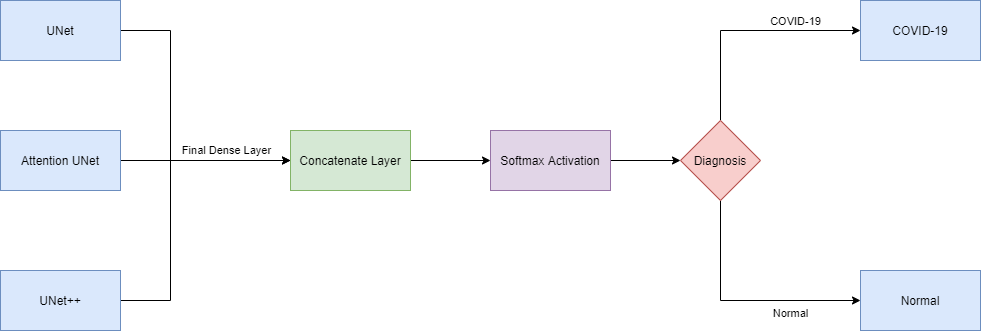
\includegraphics[width=15.5cm]{Images/EnsembleCT.png}
            %\decoRule
	\caption{\small Ensemble Learning Illustration for CT Scans}
	\label{fig:ct ensemble}
\end{figure}

\subsubsection{Model Training}

We have once again utilized 10-fold cross validation to train our CT models. We have also left an eleventh fold to test our model on unseen data. As seen from Section \ref{EDA CT}, we have built a balanced dataset comprised of 3993 samples from each class (3993 is a multiple of 11). The size of the eleventh fold also referred to as \textit{unseen data}, is 363.

At each iteration of the 10-fold cross validation, 90\% of the training data undergoes the augmentation steps and the remaining 10\% is used for validation purposes.

\begin{longtable}{| p{.13\textwidth} | p{.06\textwidth} | p{.18\textwidth} | p{.15\textwidth} | p{.18\textwidth} | p{.11\textwidth} |} 

    \hline
\textbf{Disease} & \textbf{Total}    & \textbf{Non-augmented Training}   &\textbf{Augmented Training} &\textbf{Non-augmented Testing} & \textbf{Unseen Data} \\
\hline
			COVID-19    &3993   &3267    &5270   &363   &363
\\\hline
			Normal      &3993   &3267    &5270   &363   &363
\\\hline 

\caption{Dataset Distribution for CT Scans}

  \label{tab:CT Dataset Info}
    \end{longtable}
\vspace{-1em}

Augmentation of 3267 samples from each class resulted in 5270 samples as our augmented training dataset. Our final training dataset is therefore comprised of 10,540 samples as we have two classes, COVID-19 and Normal. Indeed, only the training dataset was augmented, our testing dataset was left aside only for validation purposes. Table \ref{tab:CT Dataset Info} displays the size of our data.

We have trained our UNet and Attention UNet models for 200 epochs each, whereas for UNet++ it took around 300 epochs to achieve convergence. The batch size was 1024 samples per forward/backward pass. Our ensemble model was trained for 50 epochs to give it an opportunity to learn from the final dense layers from each of our base models before returning a prediction. Similar to X-ray scans, we have initialized the same callbacks, and returned the classification report \cite{SCR} and confusion matrix \cite{SCM} after every fold which allowed us to determine the best performing model.

% A sample snippet of code is provided below.

% \vspace{1em}
% \begin{lstlisting}
% history = model.fit(augmentedDataX, YCatAug, validation_data = (XTrain[test], YCatVal), callbacks=[ESCallback, lrReduce, mcpSave], epochs=200, batch_size=1024)
% \end{lstlisting}

\subsubsection{Heatmap Visualization}

For interpreting our model's results we have generated heatmaps in addition to the diagnosis result. The same Grad-CAM technique utilizing Keras library \cite{KCV} was applied in the case of CT scans to highlight common characteristics in patients diagnosed with COVID-19. We have once again averaged the heatmaps produced by each of our three base models with the help of Numpy \cite{NUM} to obtain the final heatmap. We believe these heatmaps would aid radiologists in identifying the same lung characteristics more efficiently.

There was only one difference in our implementation when compared to X-rays. Given a test image, it was necessary for us to extract the lung parenchyma before proceeding with the diagnosis and generating the heatmaps. The heatmap filter generated was superimposed to our unprocessed CT input in order to highlight the most critical regions.

\subsubsection{Workflow Summary Illustration}

\begin{figure}[H]
	\centering
	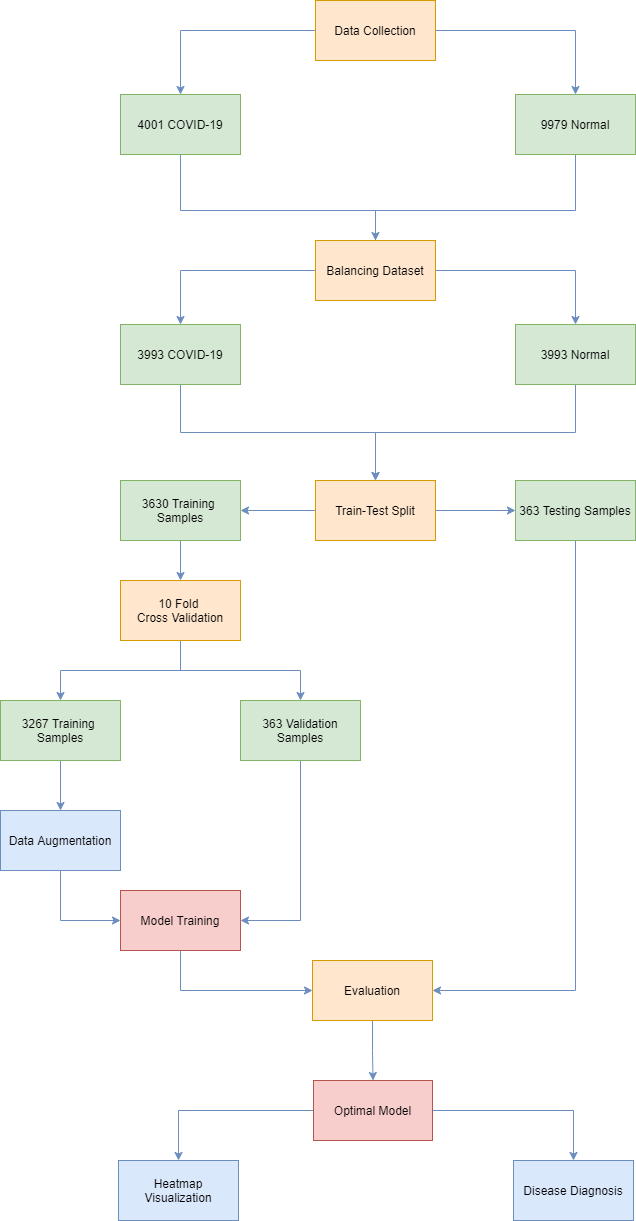
\includegraphics[width=13cm, height= 22.5cm]{Images/CT Workflow.png}

            %\decoRule
	\caption{\small CT Workflow Illustration}
	\label{fig:CT Illustration}
\end{figure}


\section{Web Interface}

Our Web Interface is a simple Diagnosis Portal allowing users to input X-ray or CT scans and retrieve real-time diagnosis and a heatmap highlighting critical regions. The front-end of the web application was built using Google's Flutter UI Toolkit. A Flask application was also deployed serving as backend containing Python scripts that retrieve diagnosis results. We have used an Ubuntu Virtual Machine offered by Microsoft Azure to deploy our Python Scripts and Web Application \footnote{Link to the Diagnosis Portal: \url{http://40.76.124.61/}}.

The Flask API provided an interface for the Flutter app, which takes the scan as input and returns diagnosis and heatmap. To ensure responsiveness of our Portal, we have utilized a custom responsive folder architecture \cite{agl2020}. We have uploaded a video demonstration of the Web Application, along with screenshots on OneDrive \footnote{Web Application Screenshots and Video Presentation can be found here: \url{https://heriotwatt-my.sharepoint.com/:f:/g/personal/agl2_hw_ac_uk/EgtAqrerqXZIhD3EPQJOJBsBJ3VTXhCZv_9pm_R01Bf8pA?e=z3mHHj}}. A subset of screenshots is displayed in Figure \ref{fig:portalScreenshots}.

\begin{figure}[H]
        \begin{subfigure}[b]{0.5\textwidth}
                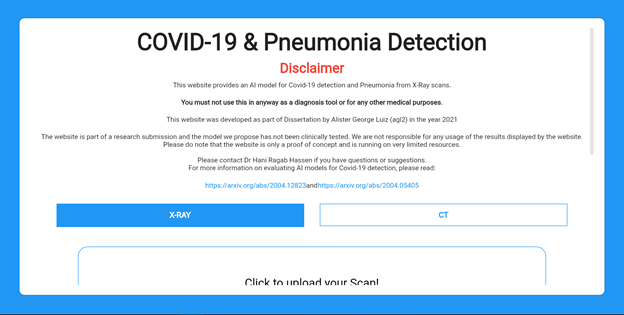
\includegraphics[width=\linewidth, height=4.3cm]{Images/Website Screenshot 1.png}
        \end{subfigure}%
        \begin{subfigure}[b]{0.5\textwidth}
                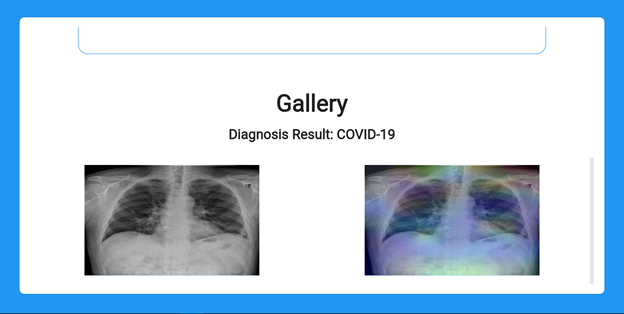
\includegraphics[width=\linewidth, height=4.3cm]{Images/Website Screenshot 2.png}
        \end{subfigure}%
        \vspace{0.8em}
        \begin{subfigure}[b]{0.5\textwidth}
                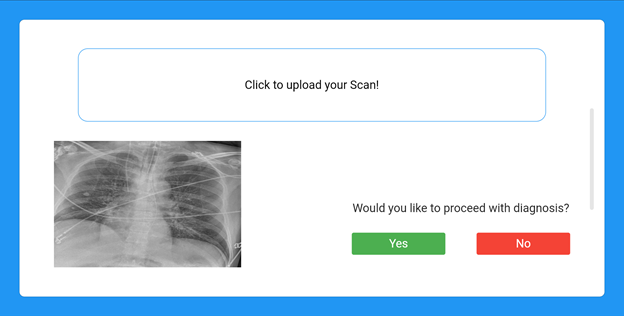
\includegraphics[width=\linewidth, height=4.3cm]{Images/Website Screenshot 5.png}
        \end{subfigure}%
        \begin{subfigure}[b]{0.5\textwidth}
                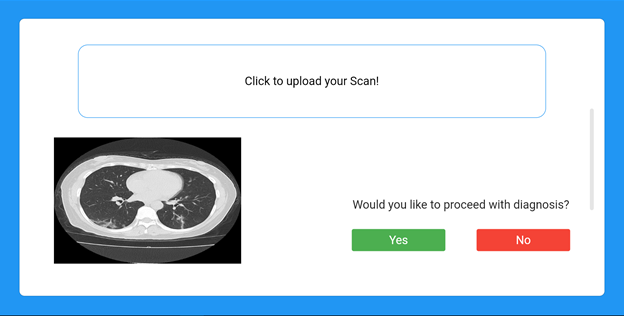
\includegraphics[width=\linewidth, height=4.3cm]{Images/Website Screenshot 7.png}
        \end{subfigure}%
        \vspace{0.8em}
        \begin{subfigure}[b]{0.5\textwidth}
                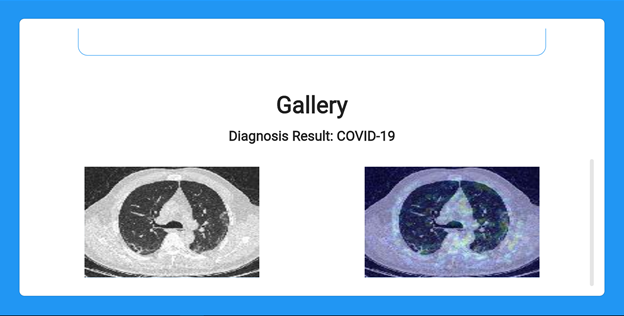
\includegraphics[width=\linewidth, height=4.3cm]{Images/Website Screenshot 3.png}
        \end{subfigure}%
        \begin{subfigure}[b]{0.5\textwidth}
                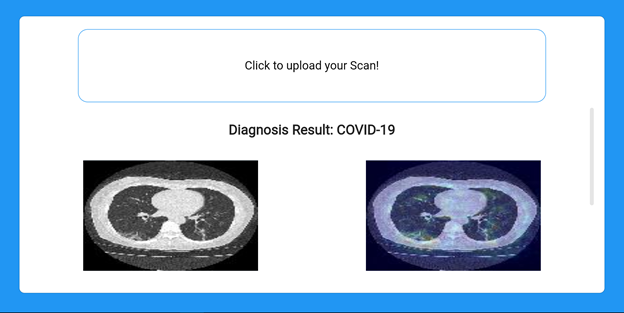
\includegraphics[width=\linewidth, height=4.3cm]{Images/Website Screenshot 8.png}
        \end{subfigure}%
        %\\\centering
        %\decoRule
        \caption{Diagnosis Portal Screenshots}\label{fig:portalScreenshots}
\end{figure}
\chapter{Results and Evaluation} \label{Results and Evaluation}

In this chapter we analyze the performance of each of our trained models. We conduct a thorough performance evaluation and compare the results obtained with the RT-PCR test and a basic CNN. We also compare our results with related work highlighted in Section \ref{LR}. The heatmaps obtained have also been compared to the findings observed by a professional Radiologist. 

\section{X-ray Scans}
The following sections evaluates results obtained by each of our X-ray models, followed by comparing them across various parameters.
% \vspace{-1em}
\subsection{Performance Evaluation}
We evaluate the performance of our three models, DenseNet121, ResNet50, and VGG16, across various metrics followed by showcasing the performance increase obtained by our Ensemble model. These sections are supplemented with tables, plots highlighting trends in loss and accuracy, and confusion matrices respectively. As we have performed 10-fold cross validation, we have obtained 10 confusion matrices whose values we have summed up to calculate average metric scores \cite{RGC2016}.
% \vspace{-1em}
\subsubsection{Pre-trained Models} \label{ptmXray}

The first model implemented is DenseNet121. Our 10-fold cross validation resulted in 94.6\% average accuracy on the balanced dataset. The average and best accuracy obtained on unseen data are 95.1\% and 96.8\% respectively. We have displayed classification report results indicating Precision, Recall, and F1-scores per class in Table \ref{tab:DenseNet CR} and confusion matrix in Figure \ref{fig:DenseNet121 Confusion Matrix},  followed by trends in accuracy and loss in Figure \ref{fig:densenetModelTraining}, of the best performing model.

\begin{table}[ht]
\begin{minipage}[b]{0.55\linewidth}
\centering
  \begin{longtable}{| p{.21\textwidth} |  p{.17\textwidth} |   p{.13\textwidth} | p{.11\textwidth} |} 
    \hline
& \textbf{Precision} & \textbf{Recall}    & \textbf{F1-Score}  \\
\hline
			COVID-19    &97.7\%   &97.7\%    &97.7\%
\\\hline
			Normal      &93.6\%   &92.7\%    &93.1\%
\\\hline 
            Pneumonia   &92.6\%       &93.5\%        &93.0\%
\\\hline

    \end{longtable}
        \vspace{0.5em}
    \begin{longtable}{| p{.52\textwidth} |  p{.13\textwidth}|} 
    \hline
    		\textbf{Accuracy}    &94.6\%
\\\hline
        \end{longtable}

    \vspace{1em}
 \captionsetup{width=.8\linewidth}
 \caption{DenseNet121 Classification Report}  \label{tab:DenseNet CR}
\end{minipage}
\begin{minipage}[b]{0.45\linewidth}
\centering
 \captionsetup{width=.8\linewidth}
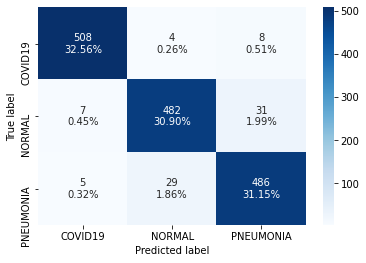
\includegraphics[width=\linewidth]{Images/DenseNetCM.png}
\captionof{figure}{DenseNet121 Confusion Matrix}
\label{fig:DenseNet121 Confusion Matrix}
\end{minipage}
\end{table}
\vspace{-\parskip}
\begin{figure}[H]
        \begin{subfigure}[b]{0.5\textwidth}
                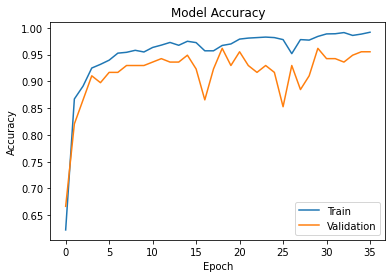
\includegraphics[width=\linewidth]{Images/DenseNetAccuracy.png}
        \end{subfigure}%
        \begin{subfigure}[b]{0.5\textwidth}
                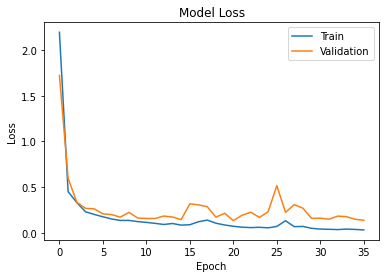
\includegraphics[width=\linewidth]{Images/DenseNetLoss.png}
        \end{subfigure}%
        %\\\centering
            %\decoRule
        \caption{DenseNet121 Model Training Performance Trends}\label{fig:densenetModelTraining}
\end{figure}
\vspace{-1em}
Next we have ResNet50 which is popular among literature as seen in Section \ref{LR}. We have achieved an average accuracy of 95.8\% after 10-fold cross validation on the balanced dataset. The average and best accuracy obtained on unseen data are 97.6\% and 98.1\% respectively. We have plotted the classification report, confusion matrix, and trends in accuracy and loss in Table \ref{tab:ResNet CR}, Figure \ref{fig:ResNet50 Confusion Matrix}, and Figure \ref{fig:resnetModelTraining} respectively.
    % \vspace{-1em}

\begin{table}[ht]
\begin{minipage}[b]{0.55\linewidth}
\centering

  \begin{longtable}{| p{.21\textwidth} |  p{.17\textwidth} |   p{.13\textwidth} | p{.11\textwidth} |} 
    \hline
& \textbf{Precision} & \textbf{Recall}    & \textbf{F1-Score}  \\
\hline
			COVID-19    &98.9\%   &99.0\%    &98.9\%
\\\hline
			Normal      &94.9\%   &93.3\%    &94.1\%
\\\hline 
            Pneumonia    &93.6\%   &95.0\%    &94.3\%
\\\hline

    \end{longtable}
        \vspace{0.5em}
    \begin{longtable}{| p{.52\textwidth} |  p{.13\textwidth}|} 
    \hline
    		\textbf{Accuracy}    &95.8\%
\\\hline
        \end{longtable}

    \vspace{1em}
     \captionsetup{width=.8\linewidth}

 \caption{ResNet50 Classification Report}  \label{tab:ResNet CR}
\end{minipage}
\begin{minipage}[b]{0.45\linewidth}
\centering
 \captionsetup{width=.8\linewidth}
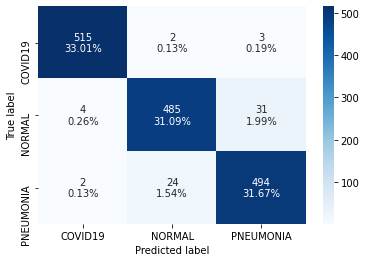
\includegraphics[width=1\linewidth]{Images/ResNetCM.png}


\captionof{figure}{ResNet50 Confusion Matrix}
\label{fig:ResNet50 Confusion Matrix}
\end{minipage}
\end{table}
\clearpage

\vspace{-\parskip}
\begin{figure}[H]
        \begin{subfigure}[b]{0.5\textwidth}
                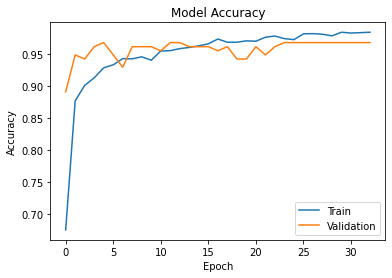
\includegraphics[width=\linewidth]{Images/ResNetAcc.png}
        \end{subfigure}%
        \begin{subfigure}[b]{0.5\textwidth}
                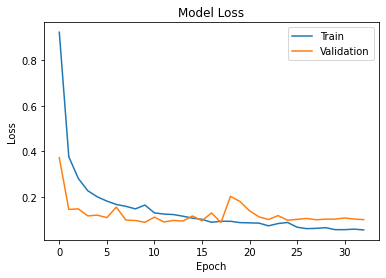
\includegraphics[width=\linewidth]{Images/ResNetLoss.png}
        \end{subfigure}%
        %\\\centering
            %\decoRule
        \caption{ResNet50 Model Training Performance Trends}\label{fig:resnetModelTraining}
\end{figure}
\vspace{-1em}
The final base model is VGG16. We have achieved an average accuracy of 95.6\% after 10-fold cross validation on the balanced dataset. The average and best accuracy obtained on unseen data are 95.3\% and 96.8\% respectively. The classification report, confusion matrix, and trends in accuracy and loss is displayed in Table \ref{tab:VGG CR}, Figure \ref{fig:VGG16 Confusion Matrix}, Figure \ref{fig:vggModelTraining} respectively.

    % \vspace{1em}

\begin{table}[ht]
\begin{minipage}[b]{0.55\linewidth}
\centering
  \begin{longtable}{| p{.21\textwidth} |  p{.17\textwidth} |   p{.13\textwidth} | p{.11\textwidth} |} 
    \hline
& \textbf{Precision} & \textbf{Recall}    & \textbf{F1-Score}  \\
\hline
			COVID-19    &97.5\%   &98.9\%    &98.2\%
\\\hline
			Normal      &94.1\%   &94.6\%    &94.3\%
\\\hline 
            Pneumonia   &95.3\%       &93.5\%        &94.4\%
\\\hline

    \end{longtable}
        \vspace{0.5em}
    \begin{longtable}{| p{.52\textwidth} |  p{.13\textwidth}|} 
    \hline
    		\textbf{Accuracy}    &95.6\%
\\\hline
        \end{longtable}

    \vspace{1em}
     \captionsetup{width=.8\linewidth}

 \caption{VGG16 Classification Report}  \label{tab:VGG CR}
\end{minipage}
\begin{minipage}[b]{0.45\linewidth}
\centering
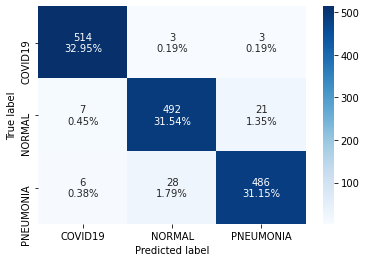
\includegraphics[width=1\linewidth]{Images/VGG16CM.png}
 \captionsetup{width=.7\linewidth}

\captionof{figure}{VGG16 Confusion Matrix}
\label{fig:VGG16 Confusion Matrix}
\end{minipage}
\end{table}


\begin{figure}[H]
        \begin{subfigure}[b]{0.5\textwidth}
                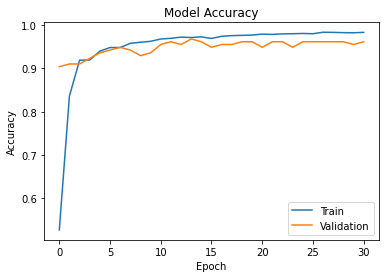
\includegraphics[width=\linewidth]{Images/VGGAcc.png}
        \end{subfigure}%
        \begin{subfigure}[b]{0.5\textwidth}
                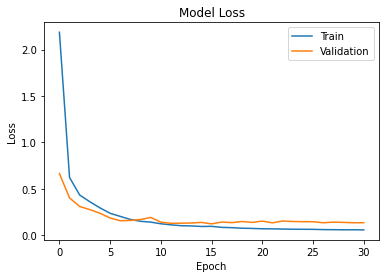
\includegraphics[width=\linewidth]{Images/VGGLoss.png}
        \end{subfigure}%
        %\\\centering
            %\decoRule
        \caption{VGG16 Model Training Performance Trends}\label{fig:vggModelTraining}
\end{figure}


\subsubsection{Ensemble Model}

After ensembling each of the three base models discussed in Section \ref{ptmXray}, we have evaluated the performance utilizing the classification report function, confusion matrix and trends in accuracy and loss. These are displayed in Table \ref{tab:EnsembleXray CR}, Figure \ref{fig:XRay Ensemble Confusion Matrix}, and Figure \ref{fig:xrayEnsembleModelTraining} respectively. We have achieved an average accuracy of 98.8\% after 10-fold cross validation on the balanced dataset. The average and best accuracy obtained on unseen data are 97.8\% and 98.1\% respectively.
    \vspace{1em}

\begin{table}[ht]
\begin{minipage}[b]{0.55\linewidth}
\centering
  \begin{longtable}{| p{.21\textwidth} |  p{.17\textwidth} |   p{.13\textwidth} | p{.11\textwidth} |} 
    \hline
& \textbf{Precision} & \textbf{Recall}    & \textbf{F1-Score}  \\
\hline
			COVID-19    &99.8\%   &99.8\%    &99.8\%
\\\hline
			Normal      &98.3\%   &98.5\%    &98.4\%
\\\hline 
            Pneumonia   &98.3\%       &98.1\%        &98.2\%
\\\hline

    \end{longtable}
        \vspace{0.5em}
    \begin{longtable}{| p{.52\textwidth} |  p{.13\textwidth}|} 
    \hline
    		\textbf{Accuracy}    &98.8\%
\\\hline
        \end{longtable}
 \captionsetup{width=.8\linewidth}
    \vspace{1em}
 \caption{X-ray Ensemble Model Classification Report}  \label{tab:EnsembleXray CR}
\end{minipage}
\begin{minipage}[b]{0.45\linewidth}
\centering
 \captionsetup{width=.8\linewidth}
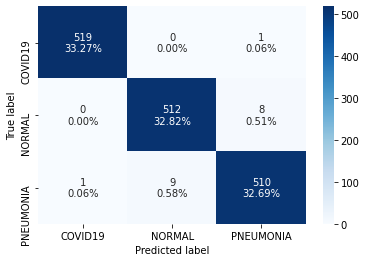
\includegraphics[width=1\linewidth]{Images/EnsembleXrayCM.png}
\captionof{figure}{X-ray Ensemble Model Confusion Matrix}
\label{fig:XRay Ensemble Confusion Matrix}
\end{minipage}
\end{table}


\begin{figure}[H]
        \begin{subfigure}[b]{0.5\textwidth}
                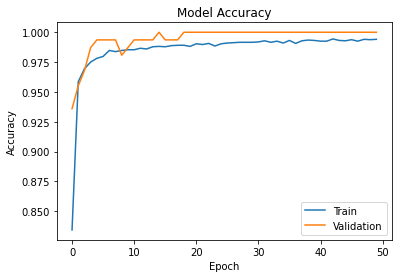
\includegraphics[width=\linewidth]{Images/EnsembleXrayAcc.png}
        \end{subfigure}%
        \begin{subfigure}[b]{0.5\textwidth}
                \includegraphics[width=\linewidth]{Images/EnsembleXrayLoss.png}
        \end{subfigure}%
        %\\\centering
            %\decoRule
        \caption{X-ray Ensemble Model Training Performance Trends}\label{fig:xrayEnsembleModelTraining}
\end{figure}


\subsection{Performance Comparison}
In the following sections we compare the performance of our models with respect to each other and determine the best performing model, followed by comparing the best results with that of the RT-PCR test and CNN. We also compare our results with related studies observed in the literature. We conclude this section by comparing our heatmap results with that of the findings obtained by a professional Radiologist who has volunteered to help us in this study.

\subsubsection{Comparison of Trained Models}

We compare each of our base X-ray models along with the ensemble model across various parameters such as Accuracy, Precision, Recall, F1-Score, Specificity, and Sensitivity respectively. The average metric scores are tabulated in Table \ref{tab:mpcXray}.

\vspace{1em}
 \begin{longtable}{| p{.23\textwidth} |  p{.1\textwidth} |   p{.1\textwidth} | p{.06\textwidth} | p{.095\textwidth} | p{.11\textwidth} | p{.11\textwidth} |} 
    \hline
& \textbf{Accuracy} & \textbf{Precision} & \textbf{Recall} & \textbf{F1-Score} & \textbf{Specificity} & \textbf{Sensitivity} \\
\hline
			DenseNet121    &94.6\%   &94.6\%    &94.6\%    &94.6\%   &97.3\%   &94.6\% 
\\\hline
			ResNet50    &95.8\%   &95.8\%    &95.8\%    &95.8\%   &97.9\%   &95.8\% 
\\\hline
			VGG16    &95.6\%   &95.6\%    &95.6\%    &95.6\%   &99.0\%   &97.8\% 
\\\hline
	        \textbf{Ensemble Model}    &\textbf{98.8\%}   &\textbf{98.8\%}    &\textbf{98.8\%}    &\textbf{98.8\%}   &\textbf{99.4\%}   &\textbf{98.8\%} 
\\\hline
 \caption{X-ray Models Performance Comparison}  \label{tab:mpcXray}

    \end{longtable}
\vspace{-1em}
We observe that out of the base models, ResNet50 and VGG16 have very comparable results with the former having a slight performance increase when compared to the latter. However, the Ensemble Model clearly outperforms each of our base models as expected.

\subsubsection{Comparison with RT-PCR and CNN}

We compare the results given by our Ensemble model, only for \textbf{COVID-19 class}, with the RT-PCR test according to the study conducted by the Infectious Diseases Society of America (IDSA) \cite{IDS2020}. We also did implement a CNN-based model to compare our model with deep learning models that use state of the art techniques.
Table \ref{tab:comp} summarizes the comparison and uses three metrics, namely accuracy, sensitivity, and specificity. 

 \begin{longtable}{| p{.15\textwidth} | p{.11\textwidth} |  p{.11\textwidth} |   p{.11\textwidth} |} 
    \hline
& \textbf{Accuracy} & \textbf{Sensitivity} & \textbf{Specificity} \\
\hline

			RT-PCR      &94.0\%   &84.2\%    &98.9\%  
\\\hline
			CNN    &93.9\%   &85.2\%    &98.2\% 
\\\hline
			\textbf{Our Approach}   &\textbf{99.9\%}   &\textbf{99.9\%}    &\textbf{99.8\%} 
\\\hline
 \caption{Comparison with RT-PCR and CNN for X-ray scans}  \label{tab:comp}
    \end{longtable}
\vspace{-1em}
As expected, our Ensemble model performs significantly better when compared to a basic CNN model. More importantly, our approach also exhibits better performance when compared to the traditional RT-PCR test.

\subsubsection{Comparison with Related Work}

In this section, we compare the performance of the Ensemble model with similar studies found in literature. We shall compare the results obtained by our best performing model with the scores reported by studies discussed in Section \ref{LR}. Table \ref{tab:relWorkXray} tabulates these results.

\vspace{1em}
 \begin{longtable}{| p{.23\textwidth} |  p{.1\textwidth} |   p{.1\textwidth} | p{.06\textwidth} | p{.095\textwidth} | p{.11\textwidth} | p{.11\textwidth} |} 
    \hline
& \textbf{Accuracy} & \textbf{Precision} & \textbf{Recall} & \textbf{F1-Score} & \textbf{Specificity} & \textbf{Sensitivity} \\
\hline
Wang et al. \cite{LWA2020}   &83.5\%    &98.9\%     &91.0\%   &94.7\%    &99.5\%     &91.0\%
\\\hline

Ghoshal et al. \cite{GHT2020}   &92.9\%    &66.7\%     &85.7\%   &75.0\%    &99.4\%     &85.7\%
\\\hline
Zhang et al. \cite{ZXS+2020}   &96.0\%    &59.6\%     &96.0\%   &73.5\%    &70.7\%     &96.0\%
\\\hline
Narin et al. \cite{AKP2020}   &98.0\%    &76.5\%     &91.8\%   &83.5\%    &96.6\%     &91.8\%
\\\hline
    \textbf{Ensemble Model}    &\textbf{98.8\%}   &\textbf{98.8\%}    &\textbf{98.8\%}    &\textbf{98.8\%}   &\textbf{99.4\%}   &\textbf{98.8\%}  
\\\hline
 \caption{Comparison with Related Work}  \label{tab:relWorkXray}

    \end{longtable}
\vspace{-2em}

Our X-ray Ensemble model outperforms the results obtained by other studies across most metrics. We believe that various approaches considered such as Data Augmentation, Transfer Learning, and Ensemble Learning have helped our models achieve optimal classification performance.
\vspace{-1em}

\subsubsection{Comparison with Radiologist Findings} \label{rfxray}

To further verify that the heatmaps produced by the model are in conformance with the observed COVID-19 characteristics, we have provided a subset of X-rays scans to a senior Radiologist \footnote{The authors thank Dr. G.R. Mahadevan (MD, IDCCM,D.Diab, Specialist in COVID-19) from Maya Nursing Home,Tamil Nadu for annotating the X-ray and CT images.} and have asked to highlight the critical regions and provide their diagnosis results. 

Table \ref{tab:radioFinding} compares the Radiologist's annotations and diagnosis with those produced by our model along with the heatmap result.
We can observe that the heatmaps are in direct compliance with the Radiologists’ findings. Precisely, visually, the heatmaps show that our predictive model highlights at least one or more of the critical regions identified by the Radiologist. Furthermore, all areas highlighted by the Radiologist are shades of either red of purple, but never blue.

We have also verified that the heatmaps we obtained correspond to the regions highlighted from studies conducted by Harmon et al. \cite{HSX+2020} and Li et al. \cite{LLL+2020}. The lower lung lobes seem to be the most affected in patients diagnosed with COVID-19, this correlates with the observations from Chung et al. \cite{CMA+2020} and therefore, provides additional validation that lung characteristics such as GGO’s, consolidations, and lesions are major contributing factors to COVID-19 detection.

% \vspace{1em}

\begin{longtable} { | c | c | c | }
    \hline
    \textbf{Original} & \textbf{Radiologist Finding} & \textbf{Heatmap} \\ \hline
    \begin{minipage}{.3\textwidth}
    \vspace{1em}
      \includegraphics[width=\linewidth, height=30mm]{Images/PneumoniaOrig1.jpg}
    \vspace{0.5em}
    \end{minipage}
    &
  \begin{minipage}{.3\textwidth}
      \vspace{1em}
      \includegraphics[width=\linewidth, height=30mm]{Images/PneuRadio1.png}
           \centering  Pneumonia
               \vspace{0.5em}
    \end{minipage}
    & 
    \begin{minipage}{.3\textwidth}
        \vspace{1em}
      \includegraphics[width=\linewidth, height=30mm]{Images/PneumoniaHeatmap1.jpg}
      \centering Pneumonia
          \vspace{0.5em}
    \end{minipage}
    \\ \hline
        \begin{minipage}{.3\textwidth}
    \vspace{1em}
      \includegraphics[width=\linewidth, height=30mm]{Images/PneumoniaOrig2.jpg}
    \vspace{0.5em}
    \end{minipage}
    &
  \begin{minipage}{.3\textwidth}
      \vspace{1em}
      \includegraphics[width=\linewidth, height=30mm]{Images/PneuRadio2.png}
           \centering  Pneumonia
               \vspace{0.5em}
    \end{minipage}
    & 
    \begin{minipage}{.3\textwidth}
        \vspace{1em}
      \includegraphics[width=\linewidth, height=30mm]{Images/PneuHeatmap2.jpg}
      \centering Pneumonia
          \vspace{0.5em}
    \end{minipage}
    \\ \hline
    \begin{minipage}{.3\textwidth}
    \vspace{1em}
      \includegraphics[width=\linewidth, height=30mm]{Images/PneuOrig3.jpg}
    \vspace{0.5em}
    \end{minipage}
    &
  \begin{minipage}{.3\textwidth}
      \vspace{1em}
      \includegraphics[width=\linewidth, height=30mm]{Images/PneuRadio3.png}
           \centering  Pneumonia
               \vspace{0.5em}
    \end{minipage}
    & 
    \begin{minipage}{.3\textwidth}
        \vspace{1em}
      \includegraphics[width=\linewidth, height=30mm]{Images/PneuHeatmap3.jpg}
      \centering Pneumonia
          \vspace{0.5em}
    \end{minipage}
    \\ \hline
          \begin{minipage}{.3\textwidth}
    \vspace{1em}
      \includegraphics[width=\linewidth, height=30mm]{Images/covidOrig1.jpg}
    \vspace{0.5em}
    \end{minipage}
    &
  \begin{minipage}{.3\textwidth}
      \vspace{1em}
      \includegraphics[width=\linewidth, height=30mm]{Images/covidRadio1.png}
           \centering  COVID-19
               \vspace{0.5em}
    \end{minipage}
    & 
    \begin{minipage}{.3\textwidth}
        \vspace{1em}
      \includegraphics[width=\linewidth, height=30mm]{Images/covidHeatmap1.jpg}
      \centering COVID-19
          \vspace{0.5em}
    \end{minipage}
    \\ \hline
          \begin{minipage}{.3\textwidth}
    \vspace{1em}
      \includegraphics[width=\linewidth, height=30mm]{Images/covidOrig2.jpg}
    \vspace{0.5em}
    \end{minipage}
    &
  \begin{minipage}{.3\textwidth}
      \vspace{1em}
      \includegraphics[width=\linewidth, height=30mm]{Images/covidRadio2.png}
           \centering  COVID-19
               \vspace{0.5em}
    \end{minipage}
    & 
    \begin{minipage}{.3\textwidth}
        \vspace{1em}
      \includegraphics[width=\linewidth, height=30mm]{Images/covid19Heatmap2.jpg}
      \centering COVID-19
          \vspace{0.5em}
    \end{minipage}
    \\ \hline
  \caption{Comparison with Radiologist Finding}\label{tab:radioFinding}
\end{longtable}



\section{CT Scans}

In this section we conduct a comprehensive evaluation and comparison of the performance across each of our CT models.
    \vspace{-1em}
\subsection{Performance Evaluation}

The following sections evaluates the performance of each of our base models, UNet, Attention UNet, and UNet++. We have supplemented these sections with tables, plots indicating the trends in loss and accuracy, and confusion matrices respectively. 
    \vspace{-1em}

\subsubsection{Pre-trained Models}

The first model we have experimented with is UNet. We have achieved an average accuracy of 94.9\% after performing 10-fold cross validation on the balanced dataset. The average and best accuracy obtained on unseen data are 94.6\% and 95.7\% respectively. The classification report, confusion matrix, and trends in accuracy and loss have been displayed in Table \ref{tab:UNet CR}, Figure \ref{fig:UNet Confusion Matrix}, and Figure \ref{fig:unetModelTraining} respectively.

    % \vspace{1em}

\begin{table}[ht]
\begin{minipage}[b]{0.55\linewidth}
\centering
  \begin{longtable}{| p{.21\textwidth} |  p{.17\textwidth} |   p{.13\textwidth} | p{.11\textwidth} |} 
    \hline
& \textbf{Precision} & \textbf{Recall}    & \textbf{F1-Score}  \\
\hline
			COVID-19    &95.2\%   &94.7\%    &94.9\%
\\\hline
			Normal      &94.7\%   &95.2\%    &94.9\%
\\\hline 

    \end{longtable}
        \vspace{0.5em}
    \begin{longtable}{| p{.52\textwidth} |  p{.13\textwidth}|} 
    \hline
    		\textbf{Accuracy}    &94.9\%
\\\hline
        \end{longtable}

    \vspace{1em}
     \captionsetup{width=.8\linewidth}

 \caption{UNet Model Classification Report}  \label{tab:UNet CR}
\end{minipage}
\begin{minipage}[b]{0.45\linewidth}
\centering
 \captionsetup{width=.8\linewidth}
\includegraphics[width=1\linewidth]{Images/UNetCM.png}
\captionof{figure}{UNet Model Confusion Matrix}
\label{fig:UNet Confusion Matrix}
\end{minipage}
\end{table}

\vspace{-\parskip}
\begin{figure}[H]
        \begin{subfigure}[b]{0.5\textwidth}
                \includegraphics[width=\linewidth]{Images/UNetAcc.png}
        \end{subfigure}%
        \begin{subfigure}[b]{0.5\textwidth}
                \includegraphics[width=\linewidth]{Images/UNetLoss.png}
        \end{subfigure}%
        %\\\centering
            %\decoRule
        \caption{UNet Model Training Performance Trends}\label{fig:unetModelTraining}
\end{figure}

Next, we trained our Attention UNet model. We achieved an average accuracy of 98.1\% after 10-fold cross validation on the balanced dataset. The average and best accuracy obtained on the unseen data are 98.3\% and 99.2\%. We have displayed the classification report, confusion matrix, and trends in accuracy and loss in Table \ref{tab:Att UNet CR}, Figure \ref{fig:Att UNet Confusion Matrix}, and Figure \ref{fig:attunetModelTraining} respectively.

    \vspace{1em}

\begin{table}[ht]
\begin{minipage}[b]{0.55\linewidth}
\centering
  \begin{longtable}{| p{.21\textwidth} |  p{.17\textwidth} |   p{.13\textwidth} | p{.11\textwidth} |} 
    \hline
& \textbf{Precision} & \textbf{Recall}    & \textbf{F1-Score}  \\
\hline
			COVID-19    &98.3\%   &97.9\%    &98.1\%
\\\hline
			Normal      &97.9\%   &98.3\%    &98.1\%
\\\hline 

    \end{longtable}
        \vspace{0.5em}
    \begin{longtable}{| p{.52\textwidth} |  p{.13\textwidth}|} 
    \hline
    		\textbf{Accuracy}    &98.1\%
\\\hline
        \end{longtable}

    \vspace{1em}
     \captionsetup{width=.8\linewidth}

 \caption{Attention UNet Model Classification Report}  \label{tab:Att UNet CR}
\end{minipage}
\begin{minipage}[b]{0.45\linewidth}
\centering
 \captionsetup{width=.8\linewidth}

\includegraphics[width=1\linewidth]{Images/AttUNetCM.png}
\captionof{figure}{Attention UNet Model Confusion Matrix}
\label{fig:Att UNet Confusion Matrix}
\end{minipage}
\end{table}
\vspace{-\parskip}

\begin{figure}[H]
        \begin{subfigure}[b]{0.5\textwidth}
                \includegraphics[width=\linewidth]{Images/AttUNetAccuracy.png}
        \end{subfigure}%
        \begin{subfigure}[b]{0.5\textwidth}
                \includegraphics[width=\linewidth]{Images/AttUNetLoss.png}
        \end{subfigure}%
        %\\\centering
            %\decoRule
        \caption{Attention UNet Model Training Performance Trends}\label{fig:attunetModelTraining}
\end{figure}

The last model we have evaluated is UNet++. We have achieved an average accuracy of 90.2\% after 10-fold cross validation on the balanced dataset. The average and best accuracy obtained on the unseen data are 88.0\% and 91.2\% respectively. We have displayed the classification report, confusion matrix, and trends in loss and accuracy in Table \ref{tab:UNet++ CR}, Figure \ref{fig:UNet++ Confusion Matrix}, and Figure \ref{fig:unet++ModelTraining} respectively.


    % \vspace{1em}

\begin{table}[ht]
\begin{minipage}[b]{0.55\linewidth}
\centering
  \begin{longtable}{| p{.21\textwidth} |  p{.17\textwidth} |   p{.13\textwidth} | p{.11\textwidth} |} 
    \hline
& \textbf{Precision} & \textbf{Recall}    & \textbf{F1-Score}  \\
\hline
			COVID-19    &92.9\%   &88.1\%    &90.5\%
\\\hline
			Normal      &88.1\%   &92.9\%    &90.5\%
\\\hline 

    \end{longtable}
        \vspace{0.5em}
    \begin{longtable}{| p{.52\textwidth} |  p{.13\textwidth}|} 
    \hline
    		\textbf{Accuracy}    &90.2\%
\\\hline
        \end{longtable}

    \vspace{1em}
     \captionsetup{width=.7\linewidth}

 \caption{UNet++ Model Classification Report}  \label{tab:UNet++ CR}
\end{minipage}
\begin{minipage}[b]{0.45\linewidth}
\centering
 \captionsetup{width=.8\linewidth}

\includegraphics[width=1\linewidth]{Images/UNet++CM.png}
\captionof{figure}{UNet++ Model Confusion Matrix}
\label{fig:UNet++ Confusion Matrix}
\end{minipage}
\end{table}
\vspace{-\parskip}
\begin{figure}[H]
        \begin{subfigure}[b]{0.5\textwidth}
                \includegraphics[width=\linewidth]{Images/UNet++Accuracy.png}
        \end{subfigure}%
        \begin{subfigure}[b]{0.5\textwidth}
                \includegraphics[width=\linewidth]{Images/UNet++Loss.png}
        \end{subfigure}%
        %\\\centering
            %\decoRule
        \caption{UNet++ Model Training Performance Trends}\label{fig:unet++ModelTraining}
\end{figure}

\vspace{-3em}
\subsubsection{Ensemble Model}

We have ensembled each of our base CT models to further improve classification performance. We have achieved an average accuracy of 98.7\% after cross validation of the balanced dataset. The average and best accuracy obtained on unseen data are 97.9\% and 97.8\%. Table \ref{tab:CT Ensemble CR}, Figure \ref{fig:CT Ensemble Confusion Matrix}, and Figure \ref{fig:ctensembleModelTraining} displays the classification report, confusion matrix, and trends in loss and accuracy respectively.



    % \vspace{1em}

\begin{table}[ht]
\begin{minipage}[b]{0.55\linewidth}
\centering
  \begin{longtable}{| p{.21\textwidth} |  p{.17\textwidth} |   p{.13\textwidth} | p{.11\textwidth} |} 
    \hline
& \textbf{Precision} & \textbf{Recall}    & \textbf{F1-Score}  \\
\hline
			COVID-19    &98.8\%   &98.5\%    &98.7\%
\\\hline
			Normal      &98.5\%   &98.8\%    &98.7\%
\\\hline 

    \end{longtable}
        \vspace{0.5em}
    \begin{longtable}{| p{.52\textwidth} |  p{.13\textwidth}|} 
    \hline
    		\textbf{Accuracy}    &98.7\%
\\\hline
        \end{longtable}
 \captionsetup{width=.8\linewidth}

    \vspace{1em}
 \caption{CT Ensemble Model Classification Report}  \label{tab:CT Ensemble CR}
\end{minipage}
\begin{minipage}[b]{0.45\linewidth}
\centering
 \captionsetup{width=.8\linewidth}

\includegraphics[width=1\linewidth]{Images/CTEnsembleCM.png}
\captionof{figure}{CT Ensemble Model Confusion Matrix}
\label{fig:CT Ensemble Confusion Matrix}
\end{minipage}
\end{table}


\begin{figure}[H]
        \begin{subfigure}[b]{0.5\textwidth}
                \includegraphics[width=\linewidth]{Images/CTEnsembleAccuracy.png}
        \end{subfigure}%
        \begin{subfigure}[b]{0.5\textwidth}
                \includegraphics[width=\linewidth]{Images/CTEnsembleLoss.png}
        \end{subfigure}%
        %\\\centering
            %\decoRule
        \caption{CT Ensemble Model Training Performance Trends}\label{fig:ctensembleModelTraining}
\end{figure}


\subsection{Performance Comparison}

In the following sections, we compare our models amongst each other and determine the best model. We also compare the best model with the RT-PCR test and CNN, followed by similar studies from literature. Finally, we compare the heatmaps obtained with findings observed by a professional Radiologist.

\subsubsection{Comparison of Trained Models}

We compare each of our base CT models along with the ensemble model across various parameters such as Accuracy, Precision, Recall, F1-Score, Specificity, and Sensitivity respectively. The average metric scores are tabulated in Table \ref{tab:mpcCT}.

\vspace{1em}
 \begin{longtable}{| p{.23\textwidth} |  p{.1\textwidth} |   p{.1\textwidth} | p{.06\textwidth} | p{.095\textwidth} | p{.11\textwidth} | p{.11\textwidth} |} 
    \hline
& \textbf{Accuracy} & \textbf{Precision} & \textbf{Recall} & \textbf{F1-Score} & \textbf{Specificity} & \textbf{Sensitivity} \\
\hline
			UNet    &94.9\%   &94.9\%    &94.9\%    &94.9\%   &94.9\%   &94.9\% 
\\\hline
			Attention UNet    &98.1\%   &98.1\%    &98.1\%    &98.1\%   &98.1\%   &98.1\% 
\\\hline
			UNet++    &90.2\%   &90.5\%    &90.5\%    &90.5\%   &90.3\%   &90.5\% 
\\\hline
	        \textbf{Ensemble Model}    &\textbf{98.7\%}   &\textbf{98.7\%}    &\textbf{98.7\%}    &\textbf{98.7\%}   &\textbf{98.7\%}   &\textbf{98.7\%} 
\\\hline
 \caption{CT Models Performance Comparison}  \label{tab:mpcCT}

    \end{longtable}
\vspace{-1em}
We observe that out of the base models, Attention UNet outperforms the rest. As expected, a slight performance increase is also observed from the Ensemble model.

\subsubsection{Comparison with RT-PCR and CNN}

We compare the results obtained by our Ensemble model with traditional RT-PCR test and a basic CNN model, only for \textbf{COVID-19 class}. Once again, we use the study conducted by the Infectious Diseases Society of America (IDSA) \cite{IDS2020} for comparison purposes. Table \ref{tab:compCT} compares the results.

 \begin{longtable}{| p{.15\textwidth} | p{.11\textwidth} |  p{.11\textwidth} |   p{.11\textwidth} |} 
    \hline
& \textbf{Accuracy} & \textbf{Sensitivity} & \textbf{Specificity} \\
\hline

			RT-PCR      &94.0\%   &84.2\%    &98.9\%  
\\\hline
			CNN    &82.3\%   &80.2\%    &84.6\% 
\\\hline
			\textbf{Our Approach}   &\textbf{98.7\%}   &\textbf{98.5\%}    &\textbf{98.8\%} 
\\\hline
 \caption{Comparison with RT-PCR and CNN for X-ray scans}  \label{tab:compCT}
    \end{longtable}
\vspace{-1em}

We observe that our Ensemble model outperforms CNN across all metrics. We also observe that our approach performs better than traditional RT-PCR test.  

\subsubsection{Comparison with Related Work}

We compare the performance of our Ensemble model to related work discussed in Section \ref{LR} across various metrics. The results are summarized in Table \ref{tab:relWorkCT}.


\vspace{1em}
 \begin{longtable}{| p{.23\textwidth} |  p{.1\textwidth} |   p{.1\textwidth} | p{.06\textwidth} | p{.095\textwidth} | p{.11\textwidth} | p{.11\textwidth} |} 
    \hline
& \textbf{Accuracy} & \textbf{Precision} & \textbf{Recall} & \textbf{F1-Score} & \textbf{Specificity} & \textbf{Sensitivity} \\
\hline
Wang et al. \cite{WBX+2020} &79.3\%    &55.0\%     &83.0\%   &66.2\%    &67.0\%     &83.0\%
\\\hline
Jin et al. \cite{JCW+2020} &80.4\%    &95.0\%     &73.5\%   &82.9\%    &92.9\%     &73.5\%
\\\hline
Song et al. \cite{SZL+2020} &86.0\%    &81.0\%     &93.0\%   &86.6\%    &76.7\%     &93.0\%
\\\hline
Zheng et al. \cite{CXZ+2020}   &90.1\%    &84.0\%     &90.7\%   &87.2\%    &91.1\%     &90.7\%
\\\hline
Chen et al. \cite{CJL+2020}   &91.6\%    &84.6\%     &100\%   &91.6\%    &93.6\%     &100\%
\\\hline
Li et al. \cite{LLL+2020}   &94.0\%    &89.7\%     &89.7\%   &89.7\%    &95.7\%     &89.7\%
\\\hline
\textbf{Ensemble Model}    &\textbf{98.7\%}   &\textbf{98.7\%}    &\textbf{98.7\%}    &\textbf{98.7\%}   &\textbf{98.7\%}   &\textbf{98.7\%} 
\\\hline
 \caption{Comparison with Related Work}  \label{tab:relWorkCT}

    \end{longtable}
\vspace{-1em}

Our Ensemble model performs significantly better when compared other approaches across all metrics. Once again, the data pre-processing and processing workflow such as splitting the lung parenchyma, augmentation, transfer learning, and ensemble learning respectively, seems to play a major factor to the models optimal performance.


\subsubsection{Comparison with Radiologist Findings}

We once again compare the generated heatmaps with that of the findings observed by a professional Radiologist. From Table \ref{tab:radioFindingCT}, we can observe that the heatmaps generated are in direct conformance with the senior Radiologist's finding \footnote{The authors thank Dr. G.R. Mahadevan (MD, IDCCM,D.Diab, Specialist in COVID-19) from Maya Nursing Home,Tamil Nadu for annotating the X-ray and CT images.}. The heatmaps identify at least one or more of the critical regions highlighted by the Radiologist. We also observe that all areas highlighted by the Radiologist are shades of red, purple, or green and not blue. 

Furthermore, similar to our observations from Section \ref{rfxray}, we have verified that our heatmaps correlate to the studies conducted by Harmon et al., Li et al., and Chung et al., therefore ensuring the reliability of our results. We observe that consolidations, GGO's, and lesions are major contributing factors to COVID-19 detection.

\begin{longtable} { | c | c | c | }
    \hline
    \textbf{Original} & \textbf{Radiologist Finding} & \textbf{Heatmap} \\ \hline
    \begin{minipage}{.3\textwidth}
    \vspace{1em}
      \includegraphics[width=\linewidth, height=30mm]{Images/ctOrig1.png}
    \vspace{0.5em}
    \end{minipage}
    &
  \begin{minipage}{.3\textwidth}
      \vspace{1em}
      \includegraphics[width=\linewidth, height=30mm]{Images/ctRadio1.png}
           \centering  COVID-19
               \vspace{0.5em}
    \end{minipage}
    & 
    \begin{minipage}{.3\textwidth}
        \vspace{1em}
      \includegraphics[width=\linewidth, height=30mm]{Images/ctHeatmap1.jpg}
      \centering COVID-19
          \vspace{0.5em}
    \end{minipage}
    \\ \hline
    \begin{minipage}{.3\textwidth}
    \vspace{1em}
      \includegraphics[width=\linewidth, height=30mm]{Images/ctOrig2.png}
    \vspace{0.5em}
    \end{minipage}
    &
  \begin{minipage}{.3\textwidth}
      \vspace{1em}
      \includegraphics[width=\linewidth, height=30mm]{Images/ctRadio2.png}
           \centering  COVID-19
               \vspace{0.5em}
    \end{minipage}
    & 
    \begin{minipage}{.3\textwidth}
        \vspace{1em}
      \includegraphics[width=\linewidth, height=30mm]{Images/ctHeatmap2.jpg}
      \centering COVID-19
          \vspace{0.5em}
    \end{minipage}
     \\ \hline
    \begin{minipage}{.3\textwidth}
    \vspace{1em}
      \includegraphics[width=\linewidth, height=30mm]{Images/ctOrig3.png}
    \vspace{0.5em}
    \end{minipage}
    &
  \begin{minipage}{.3\textwidth}
      \vspace{1em}
      \includegraphics[width=\linewidth, height=30mm]{Images/ctRadio3.png}
           \centering  COVID-19
               \vspace{0.5em}
    \end{minipage}
    & 
    \begin{minipage}{.3\textwidth}
        \vspace{1em}
      \includegraphics[width=\linewidth, height=30mm]{Images/ctHeatmap3.jpg}
      \centering COVID-19
          \vspace{0.5em}
    \end{minipage}
      \\ \hline
  \caption{Comparison with Radiologist Finding}\label{tab:radioFindingCT}

\end{longtable}

\section{Web Interface}
In this section, we highlight the results obtained by the Usability Study we have conducted. It is of utmost importance to understand and measure the usability of the COVID-19 and Pneumonia Diagnosis Platform. The feedback received would be really beneficial for future iterations of this application in terms of design improvements and feature additions.

\subsection{Hypothesis} \label{hypo}

\textit{Through this experiment, Alister George Luiz (the investigator) is attempting to prove that the
COVID-19 and Pneumonia Diagnosis Platform is usable in the sense that it is user-friendly, consistent, familiar, responsive, and intuitive.}

\subsection{Target Audience}

Any user, with or without technical experience, in any age group was eligible for this study. A consent form was provided virtually to comply with the compulsory policy of no face-to-face interactions due to the outbreak of the pandemic. All the terms and conditions were presented before the participant undertook the survey and was given freedom to accept or decline participation. The consent form was taken from the resources provided by the F20PA course page.

\subsection{Experiment Design}
The main motive behind designing a Usability Study was due to the fact that the COVID-19 and Pneumonia Diagnosis Platform is a user-facing product. The purpose of this user study was to \textbf{quantitatively} and \textbf{qualitatively} understand the perspective of the user towards our final product. Our experiment is composed of three activities. The investigator ensured that the participants viewed the video demonstration of the Diagnosis Portal and also provided Screenshots covering all aspects of the website. We have utilized Microsoft Forms  \footnote{The Microsoft Forms Link containing the Survey can be found here: \url{https://forms.office.com/r/vFuJ0VCXe5}} to conduct this study.

\subsection{Activity 1: Tasks}

In the first activity, we have asked the participants several questions after they have viewed the video demonstration. The goal of this activity was to verify that the basic system functionality is easily understandable and that they could perform these tasks without intervention from the investigator or any similar secondary help. 

The outcome of each question was either a yes or no to evaluate the participants understandability. Besides this, the investigator also welcomed feedback on the existing systems, which may be considered in future versions of this Web Portal. It is worth to note that participants were given a brief explanation of the project in the beginning of the study, and any questions were welcome via email or other messaging sources. 

We have asked this question to participants before the activity - \textbf{How frequently do you use a Computer?}

All users provided 'Daily' as their response. The main purpose of this question was to understand the influence of familiarity with computers in their respective ease of understanding of the system. We found that 
participants with daily usage of computers are usually more technically adept and can easily comprehend the system workflow. Table \ref{act:1} displays the questions and results obtained for Activity 1. 

\begin{longtable}{| p{.055\textwidth} | p{.75\textwidth} | p{.04\textwidth} | p{.03\textwidth} |} 
    \hline
    		\textbf{Q.No}    &\textbf{Question} & \textbf{Yes}     & \textbf{No}
\\\hline
            1   &Would you be able to utilize the functionality of this website independently?  &15  &0
\\\hline
            2   &Were you able to comprehend the Disclaimer message easily?  &15  &0
\\\hline
            3   &Were you able to identify where to upload the scan easily?  &15  &0
\\\hline
            4   &Were you able to understand that the slideshow showcased previous diagnosis results obtained from the portal for both COVID-19 and Pneumonia?  &13  &2
\\\hline
            5   &Were you able to identify the use of the toggle button between X-ray and CT scan?  &15  &0
\\\hline

\caption{Activity 1 Results} \label{act:1}
        \end{longtable}

The results obtained indicates that most of the participants easily understood the basic functionality and workflow of this Diagnosis Portal. Three participants could not recognize that the Gallery section showcased previous diagnosis results obtained from the portal. We believe adding a more explicit description would help in better understanding of the Gallery section.

Besides these questions, the participant was also asked to provide feedback if they felt so regarding the interface or any general suggestions. Table \ref{feedback} highlights some of the top suggestions provided, which would be definitely considered in future versions of this Diagnosis Portal.

\vspace{1em}
\begin{longtable}{| p{.055\textwidth} | p{.89\textwidth} |} 
    \hline
    		\textbf{S.No}    &\textbf{Suggestions for Improvement} 
\\\hline
            1   &Improvements to UI, Multi-page Site as in separate page for COVID-19 and Pneumonia.
\\\hline
            2   &Just keep adjusting the layout of the website so rather than scrolling all site content are seen together. Also since it's a diagnosis web portal, for future works integrating different medical issues related to COVID-19 can be trained in the AI, for more efficient outcomes.
\\\hline
            3   &If the result of the diagnosis indicates COVID - 19, guidelines and measures (according to region) being presented along with it would be helpful.
\\\hline
          4   &The options for switching between X-ray and CT could be renamed as "Click here to view X-ray" and "Click here to view CT Scan".
\\\hline

\caption{Feedback on the Diagnosis Portal} \label{feedback}
        \end{longtable}

It is indeed possible to extract relevant functionality improvements from the general feedback. Revision in User Interface, adding more information related to COVID-19, providing guidelines and measures pertaining to the region and so on are high in our priority list. We thank the participants for providing such valuable feedback.

\subsection{Activity 2: System Usability Scale (SUS) Survey}

Next, we have utilized the System Usability Scale which is a renowned and widely used tool to measure the usability of the system \cite{SUS2021, JBR1986}. We successfully completed the usability testing with fifteen participants. 

The System Usability Scale (SUS) comprised of ten questions. Each participant had to provide a rating between 1 to 5 which indeed correlated to \textbf{Strongly Disagree} and \textbf{Strongly Agree}. One interesting aspect of using the SUS was that we could easily average out the results from each participant and obtain the general consensus. The standard SUS formula was used to compute the final scores \cite{THO2015} for each participant. The questions are displayed in Table \ref{susQ} and the results obtained from each participant along with the scores is provided in Table \ref{susScores}.

\begin{longtable}{| p{.055\textwidth} | p{.83\textwidth} |} 
    \hline
    		\textbf{Q.No}    &\textbf{Question} 
\\\hline
            1   &I think that I would like to use this system frequently. Given that feedback on the results obtained by the portal must be validated by a medical professional. 
\\\hline
2   &I found this system unnecessarily complex. 
\\\hline
3   &I thought this system was easy to use. 
\\\hline
4   &I think that I would need assistance to be able to use the system. 
\\\hline
5   &I found the various functions in this system were well integrated. 
\\\hline
6   &I thought there was too much inconsistency in this system. 
\\\hline
7   &I would imagine that most people would learn to use this system very quickly.
\\\hline
8   &I found this system very cumbersome/awkward to use.
\\\hline
9   &I feel very confident using this system.
\\\hline
10  &I needed to learn a lot of things before I could get going with this system.
\\\hline

\caption{System Usability Scale (SUS) Questions} \label{susQ}
        \end{longtable}
\vspace{-1em}
\begin{longtable}{| p{.12\textwidth} | p{.03\textwidth} | p{.03\textwidth} | p{.03\textwidth} | p{.03\textwidth} | p{.03\textwidth} | p{.03\textwidth} | p{.03\textwidth} | p{.03\textwidth} | p{.03\textwidth} | p{.04\textwidth} | p{.06\textwidth} |} 
    \hline
    		\textbf{Participant}    &\textbf{Q1}    &\textbf{Q2}    &\textbf{Q3}    &\textbf{Q4}    &\textbf{Q5}    &\textbf{Q6}   &\textbf{Q7}    &\textbf{Q8}    &\textbf{Q9}    &\textbf{Q10}   &\textbf{Score} 
\\\hline
P1   &4   &1   &4   &1   &5   &1   &5   &1   &4   &1   &92.5 \\\hline
P2   &5   &1   &5   &2   &4   &1   &4   &1   &5   &1   &92.5 \\\hline
P3   &5   &1   &5   &1   &5   &1   &5   &1   &5   &1   &100 \\\hline
P4   &5   &1   &5   &1   &5   &1   &4   &2   &5   &1   &95 \\\hline
P5   &5   &1   &5   &1   &3   &1   &5   &1   &5   &1   &95 \\\hline
P6   &5   &2   &5   &1   &5   &1   &5   &2   &5   &1   &95 \\\hline
P7   &3   &1   &4   &1   &3   &1   &3   &1   &3   &1   &77.5 \\\hline
P8   &5   &1   &5   &1   &5   &1   &5   &1   &5   &1   &100 \\\hline
P9   &4   &2   &4   &1   &3   &1   &4   &1   &4   &1   &95 \\\hline
P10  &5   &1   &5   &1   &4   &2   &5   &1   &5   &1   &95 \\\hline
P11  &5   &1   &5   &2   &5   &1   &4   &1   &4   &1   &92.5 \\\hline
P12  &5   &1   &5   &1   &5   &2   &5   &1   &5   &1   &97.5 \\\hline
P13  &2   &1   &4   &2   &3   &1   &4   &1   &4   &1   &77.5 \\\hline
P14  &4   &2   &5   &1   &4   &2   &4   &1   &3   &2   &80 \\\hline
P15  &3   &2   &4   &2   &4   &2   &4   &2   &3   &2   &70 \\\hline
\caption{System Usability Scale (SUS) Scores} \label{susScores}
\end{longtable}


The average SUS score is \textbf{90.3}. As per Jeff Sauro, a SUS score above 68 is \textbf{Above Average}. A score above 80.3 is \textbf{Excellent}. As per our this criteria, we are pleased to know that our Diagnosis Portal falls into the latter category. Figure \ref{fig:susScore} displays our SUS scores and the average score. We also believe that the Mode statistical quantity is in fact really useful in understanding the participants general mindset. Therefore, we have highlighted the Mode, Maximum and Minimum per question in Table \ref{susStats}. 

\begin{figure}[H]
    \centering
    \includegraphics[height=7cm]{Images/SUSScore.png}
    %\decoRule
    \caption{Comparison of SUS Scores}
    \label{fig:susScore}
    \end{figure}
\begin{longtable}{| p{.11\textwidth} | p{.03\textwidth} | p{.03\textwidth} | p{.03\textwidth} | p{.03\textwidth} | p{.03\textwidth} | p{.03\textwidth} | p{.03\textwidth} | p{.03\textwidth} | p{.03\textwidth} | p{.04\textwidth} |} 
    \hline
    		\textbf{Statistic}    &\textbf{Q1}    &\textbf{Q2}    &\textbf{Q3}    &\textbf{Q4}    &\textbf{Q5}    &\textbf{Q6}   &\textbf{Q7}    &\textbf{Q8}    &\textbf{Q9}    &\textbf{Q10}   
\\\hline
Mode        &5   &1   &5   &1   &5   &1   &5   &1   &5   & 1 
\\\hline
Maximum     &5   &2   &5   &2   &5   &2   &5   &2   &5   &2  
\\\hline
Minimum     &2   &1   &4   &1   &3   &1   &3   &1   &3   &1  
\\\hline
\caption{System Usability Scale (SUS) Statistical Analysis} \label{susStats}
\end{longtable}

\subsection{Activity 3: Metrics Test}

The last activity involves explicitly testing the certain metrics stated in Section \ref{hypo} and Table \ref{tab:Evaluation Strategy}. We have asked the participants to fill in a Likert Scale with each metric having scores ranging from Very Poor to Excellent. Table \ref{metricTest} summarizes the results. 

\begin{longtable}{| p{.19\textwidth} | p{.11\textwidth} | p{.05\textwidth} | p{.04\textwidth} | p{.06\textwidth} | p{.10\textwidth} |} 
    \hline
    		\textbf{Metric}    &\textbf{Very Poor}    &\textbf{Poor}    &\textbf{Fair}    &\textbf{Good}    &\textbf{Excellent}
\\\hline
User-Friendliness  &0   &0   &1   &7  &7   
\\\hline
Consistency  &0   &0   &1   &8   &6  
\\\hline
Familiarity  &0   &0   &5   &7   &3   
\\\hline
Responsiveness  &0   &0   &0   &7   &8   
\\\hline
Intuitiveness  &0   &0   &1   &11   &3   
\\\hline
Overall User Experience  &0   &0   &0   &8   &7   
\\\hline

\caption{Activity 3 Likert Scale Results} \label{metricTest}
\end{longtable}

We are pleased to note that all of the participants ranked each metric above 'Fair'. We also note that system familiarity as higher 'Fair' number, therefore, we plan to improve this metric by scouting the user interface of web applications with similar functionality. We believe having a user interface similar to popular pre-existing web applications would improve the familiarity of the Diagnosis Portal with its users. 

\section{Requirements Validation} \label{reqVal}

In this section, we confirm that all the requirements stated at the inception of this project is satisfied. Table \ref{tab:Requirements Validation} tabulates our requirements and their status of completion.
\vspace{1em}
\begin{longtable}{| p{.05\textwidth} | p{.60\textwidth} | p{.08\textwidth} | p{.12\textwidth} |} 
\hline
\multicolumn{4}{|c|}{\textbf{Functional Requirements}}\\
\hline
\textbf{ID} & \textbf{Description} & \textbf{Priority} & \textbf{Status}  \\
\hline
FR-1 & \textbf{X-ray Segmentation}  & \cellcolor{green}\textbf{M} & Completed \\ &  The system shall be able to accept and segment X-ray scans. & \cellcolor{green} &  \\ \hline 
FR-2 & \textbf{CT Segmentation}  & \cellcolor{cyan}\textbf{S} & Completed\\ &  The system shall be able to accept and segment CT scans. & \cellcolor{cyan} &  \\ \hline 
FR-3 & \textbf{COVID-19 Diagnosis using X-ray Scans}  & \cellcolor{green}\textbf{M} & Completed\\ & The system shall be able to classify positive COVID-19 patients from others given test X-ray scans & \cellcolor{green} & \\ \hline 
FR-4 & \textbf{COVID-19 Diagnosis using CT Scans}  & \cellcolor{cyan}\textbf{S} & Completed\\ &  The system shall be able to classify positive COVID-19 patients from others given test CT scans. & \cellcolor{cyan} & \\ \hline
FR-5 & \textbf{Visualize Lung Region of Interest's}  & \cellcolor{green}\textbf{M} & Completed\\ &  The system shall be able to interpret and visualize classification results by highlighting lung ROIs. & \cellcolor{green} & \\ \hline 
FR-6 & \textbf{Multi-class Diagnosis}  & \cellcolor{pink}\textbf{W} & Completed\\ &  The system shall be able to differentiate COVID-19 and Pneumonia (Viral or Bacterial) patients. & \cellcolor{pink} & for X-rays \\ \hline 
FR-7 & \textbf{Web Interface}  & \cellcolor{cyan}\textbf{S} & Completed\\ &  The system shall have an interface which presents diagnosis results after segmentation for visualization and analysis purposes. & \cellcolor{cyan} & \\ \hline

\caption{Requirements Validation}

  \label{tab:Requirements Validation}
  \end{longtable}

All the requirements stated from FR-1 to FR-4 has been satisfied through our implementation workflow. The segmentation is carried out during data preparation, especially in the case of CT scans where we extract the lung parenchyma and by our state-of-the-art deep learning models during model training. Indeed, the diagnosis is carried out when our models return their prediction after processing the input scan. Therefore, satisfying these requirements.

Through our Grad-CAM visualization, we are able to interpret and visualize classification results by viewing the highlighted ROI's, therefore satisfying FR-5. For multi-class diagnosis, that is, FR-6, in addition to COVID-19 diagnosis, we have also been able to successfully diagnose patients with Pneumonia using X-ray scans. This was indeed possible due to the availability of an open-source dataset consisting of both COVID-19 and Pneumonia X-ray scans. Unfortunately, as we were not able to find an open source dataset consisting of CT scans from Pneumonia patients, we have performed binary classification utilizing COVID-19 and Normal samples.

The last requirement, FR-7, was satisfied through our Flutter web application, which allows users to input their chest X-ray or CT scans and receive real-time diagnosis along with the critical regions highlighted via the heatmaps generated.  
\chapter{Conclusion and Future Work} \label{Conclusion and Future Works}

This chapter concludes this manuscript and provides additional information on where to find the source code, the limitations of this project, future works we wish to undertake and finally my thoughts and reflections on my experiences throughout this year long project.

\section{Limitations}

Despite our best efforts there are indeed some limitations to this project implementation which could be overcome in future iterations. The first being the availability of a reasonably sized dataset. We have noticed that there have only been a handful of researchers and institutions actively collecting chest X-rays and CT scans with most of the data not being open-source. Therefore, most of the datasets on Kaggle and other forums usually cite the same root source. Although we have performed Data Augmentation to generate more samples, we believe having more COVID-19 samples would indeed increase the reliability of our model.

The free-to-use tier of Google Colab was another major limitation in training our models. Due to the limited RAM (12GB) and runtime duration (12 hours per day), we had to incorporate memory optimization strategies such as reducing the batch size and image dimensions in order to be able to fit the data into memory and conduct training. This was especially for the case of CT scans. Furthermore, we also had a ceiling for the number of augmented images generated due to the same memory limitation.

As we have utilized the free credit offered by Microsoft Azure for students, the Ubuntu Virtual Machine used to host our Python Scripts and Flutter Web Application on their platform would only run for 2.5 months, after which a monthly fee of \$30 apply for continued use. 

\section{Future Work}

We have a lot planned in the future for this project. Provided we gain access to a powerful machine well beyond the capabilities of a standard Google Colab environment, we believe we can further increase the reliability and performance of our models. Here are a list of proposed ideas:
\begin{enumerate}
    \item \textbf{Data Sources} - Identify more data sources to increase the size of our existing dataset.
    \item \textbf{Image Dimensions} - Given a machine with higher RAM, perform model training with larger image dimensions.
    \item \textbf{Data Augmentation} - Utilize Data Augmentation to generate more samples per class.
    \item \textbf{Multi-class CT Classification} - Obtain CT scans from Pneumonia patients and build multi-class classification model.
    \item \textbf{Research Papers} - Publish research papers on our X-ray and CT scan implementation, along with a survey paper.
    \item \textbf{Radilogist Validation} - Validate more model results and heatmaps with a Radiologist and receive their feedback on the web application and thereby make suitable changes.
\end{enumerate}

\section{Reflections}

Through this year long project, I was able to gain valuable experience and improve both technical and soft skills through various phases of this project. More importantly, being my first ever major Data Science project, I was able to learn from my mistakes and overcome all the roadblocks faced with the guidance and support of my project supervisor, Dr. Hani Ragab, who was always available to clear my doubts, provide fruitful insights and resources. 

I would also like to thank Dr. Hadj Batatia and Professor Kayvan Karim for providing their thoughts and assistance towards this project. Lastly, I would also like to take a moment to thank my parents for their constant prayers and motivation throughout the project, who pushed me to achieve my goals and become the person I am today. 

I truly believe that my commitment and hard work coupled with the guidance and encouragement provided by my project supervisor, professors, and parents have led to this project reach its potential and achieve successful completion. 

\printbibliography[heading=bibintoc]

%----------------------------------------------------------------------------------------
%	THESIS CONTENT - APPENDICES
%----------------------------------------------------------------------------------------

\appendix % Cue to tell LaTeX that the following "chapters" are Appendices

% Include the appendices of the thesis as separate files from the Appendices folder
% Uncomment the lines as you write the Appendices

% Chapter Template

\chapter{Requirements Analysis and Evaluation Strategy} % Main chapter title
\label{Requirements Analysis} % Change X to a consecutive number; for referencing this chapter elsewhere, use \ref{ChapterX}

%----------------------------------------------------------------------------------------
%	SECTION 1
%----------------------------------------------------------------------------------------

This chapter provides an insight into the project requirements followed by demonstrating the project implementation workflow, UI wireframe, data collection, and processing methodology, and concludes with an evaluation strategy.

\section{Requirements Analysis}
This section identifies and outlines the functional and non-functional requirements pertaining to this project. The priority 
of each of these requirements are ranked according to the MSCW prioritization technique. The following color-scheme 
indicates the respective ranking order:

\begin{itemize}
  \item \colorbox{green}{\textbf{Must Have (M)}} - These requirements are fundamental to achieve the aim of this project.
  \item \colorbox{cyan}{\textbf{Should Have (S)}} - These requirements are important to the project but not vital and could be achieved in the long run.
  \item \colorbox{yellow}{\textbf{Could Have (C)}} - These requirements are not fundamental to achieve the aim of this project but would be an added benefit if accomplished.
  \item \colorbox{pink}{\textbf{Want To Have (W)}} - These requirements would be prioritized in later releases of the project.
\end{itemize}

\subsection{Functional and Non-Functional Requirements}
The Functional Requirements (FR's) describes the essential components, purpose, and objectives of this project.
Table \ref{tab:Functional Requirements} tabulates the FR's along with a brief description for the same and its priority according to MSCW prioritization technique. An evaluation 
for each of these functional requirements is specified in section \ref{Evaluation Strategy Section}.

% \subsection{Non-Functional Requirements}
Non-Functional Requirements (NFR's) emphasizes the system's operation which includes its performance, usability, portability, and so on. Table \ref{tab:Non-Functional Requirements} tabulates each of these NFR's and applies the MSCW prioritization technique.

\begin{longtable}{| p{.10\textwidth} | p{.70\textwidth} | p{.10\textwidth} |} 
\hline
\multicolumn{3}{|c|}{\textbf{Functional Requirements}}\\
\hline
\textbf{ID} & \textbf{Description} & \textbf{Priority}  \\
\hline
FR-1 & \textbf{X-ray Segmentation}  & \cellcolor{green}\textbf{M} \\ &  The system shall be able to accept and segment X-ray scans. & \cellcolor{green} \\ \hline 
FR-2 & \textbf{CT Segmentation}  & \cellcolor{cyan}\textbf{S} \\ &  The system shall be able to accept and segment CT scans. & \cellcolor{cyan} \\ \hline 
FR-3 & \textbf{COVID-19 Diagnosis using X-ray Scans}  & \cellcolor{green}\textbf{M} \\ & The system shall be able to classify positive COVID-19 patients from others given test X-ray scans & \cellcolor{green} \\ \hline 
FR-4 & \textbf{COVID-19 Diagnosis using CT Scans}  & \cellcolor{cyan}\textbf{S} \\ &  The system shall be able to classify positive COVID-19 patients from others given test CT scans. & \cellcolor{cyan} \\ \hline
FR-5 & \textbf{Visualize Lung Region of Interest's}  & \cellcolor{green}\textbf{M} \\ &  The system shall be able to interpret and visualize classification results by highlighting lung ROIs. & \cellcolor{green} \\ \hline 
FR-6 & \textbf{Multi-class Diagnosis}  & \cellcolor{pink}\textbf{W} \\ &  The system shall be able to differentiate COVID-19 and Pneumonia (Viral or Bacterial) patients. & \cellcolor{pink} \\ \hline 
FR-7 & \textbf{Web Interface}  & \cellcolor{cyan}\textbf{S} \\ &  The system shall have an interface which presents diagnosis results after segmentation for visualization and analysis purposes. & \cellcolor{cyan} \\ \hline

% \multirowcell{2}{FR2} & 70 COVID-19 & \cellcolor{green} \\ & Others & \multirowcell{-2}{*}{ \cellcolor{green}S}\\ \hline
\caption{Functional Requirements}

  \label{tab:Functional Requirements}
  \end{longtable}

%   \begin{longtable}{| p{.10\textwidth} | p{.70\textwidth} | p{.10\textwidth} |} 
%     \hline
%     \multicolumn{3}{|c|}{\textbf{User Functional Requirements}}\\
%     \hline
%     \textbf{ID} & \textbf{Description} & \textbf{Priority}  \\
%     \hline
%     U-FR-1 & \textbf{Input X-ray Scans}  & \cellcolor{green}\textbf{M} \\ & The user shall be able to provide X-ray scan images as input for COVID-19 diagnosis. & \cellcolor{green} \\ \hline 
%     U-FR-2 & \textbf{Input CT Scans}  & \cellcolor{cyan}\textbf{S} \\ &   The user shall be able to provide CT scan images as input for COVID-19 diagnosis. & \cellcolor{cyan} \\ \hline 
%     U-FR-3 & \textbf{Save Classification Results}  & \cellcolor{green}\textbf{M} \\ & The user shall be able to save and interact with the classification results which highlights the lung ROI's. & \cellcolor{green} \\ \hline 

%     % \multirowcell{2}{FR2} & 70 COVID-19 & \cellcolor{green} \\ & Others & \multirowcell{-2}{*}{ \cellcolor{green}S}\\ \hline
%     \caption{User Functional Requirements}
    
%       \label{tab:User Functional Requirements}
%       \end{longtable}

\vspace{5em}
% \\\\
\begin{longtable}{| p{.10\textwidth} | p{.70\textwidth} | p{.10\textwidth} |} 
  
  \hline
  \multicolumn{3}{|c|}{\textbf{Non-Functional Requirements}}\\
  \hline
  \textbf{ID} & \textbf{Description} & \textbf{Priority}  \\
  \hline
  NFR-1 & \textbf{Environment}  & \cellcolor{yellow}\textbf{C} \\ & The system shall be deployed on a cloud platform such as IBM Cloud. & \cellcolor{yellow} \\ \hline 
  NFR-2 & \textbf{User Interface}  & \cellcolor{cyan}\textbf{S} \\ &   The system shall have an intuitive and user-friendly interface evaluated via a System Usability Study where the user can input scans and receive diagnosis results which could be confirmed by a medical professional. & \cellcolor{cyan} \\ \hline 
  NFR-3 & \textbf{Extensibility}  & \cellcolor{cyan}\textbf{S} \\ & The system shall be flexible to extensions, this includes bug fixes, updated features and performance improvement.& \cellcolor{cyan} \\ \hline 
  NFR-4 & \textbf{Version Control}  & \cellcolor{green}\textbf{M} \\ & All versions of the code shall be published on GitHub which enables version control and be open source.& \cellcolor{green} \\ \hline 
  NFR-5 & \textbf{Documentation}  & \cellcolor{green}\textbf{M} \\ & The code shall include relevant comments and contain an instructions guide to setup the environment and run the code. & \cellcolor{green} \\ \hline 
  NFR-6 & \textbf{Modular Programming}  & \cellcolor{cyan}\textbf{S} \\ & The program functionality shall be separated into independent components to emphasize the scalability of software.& \cellcolor{cyan} \\ \hline 
  NFR-7 & \textbf{Reusability}  & \cellcolor{yellow}\textbf{C} \\ & The code developed shall be reusable by other researchers and developers. & \cellcolor{yellow} \\ \hline 

  % \multirowcell{2}{FR2} & 70 COVID-19 & \cellcolor{green} \\ & Others & \multirowcell{-2}{*}{ \cellcolor{green}S}\\ \hline
  \caption{Non-Functional Requirements}
  
    \label{tab:Non-Functional Requirements}
    \end{longtable}


% This chapter provides an insight into the project implementation 
% workflow, UI wireframe, data collection, and processing methodology, 
% and concludes with an evaluation strategy.
\vspace{-2em}
\section{Implementation Workflow}
The activity diagram displayed in Figure \ref{fig:Implementation Methodology} provides a blueprint of the workflow that would be followed for the development phase commencing next semester. 

% The wireframe illustrated in Appendix \ref{Wireframe} displays the expected general layout of the COVID-19 diagnosis portal.

\begin{figure}[H]
 \centering
 \includegraphics[width=15.5cm, height=11.5cm]{Images/activityDiagram.png}
%  \decoRule
 \caption[Implementation Methodology]{Activity Diagram displaying the implementation workflow.}
 \label{fig:Implementation Methodology}
 \end{figure}
 
 \vspace{-2em}
\section{Evaluation Strategy} \label{Evaluation Strategy Section}
Table \ref{tab:Evaluation Strategy} summarizes the methods and strategies used to evaluate each of the Functional Requirements described in Chapter \ref{Requirements Analysis}.

\begin{longtable}{| p{.10\textwidth} | p{.82\textwidth} |} 
\hline
\multicolumn{2}{|c|}{\textbf{Evaluation Strategy}}\\
\hline
\textbf{ID} & \textbf{Description}\\
\hline
FR-1 & \parbox[t]{12.3cm}{\textbf{X-ray Segmentation} \\ The lung segments produced from X-ray scans shall be evaluated based on its capability to identify possible ROIs.}\\\hline
FR-2 & \parbox[t]{12.3cm}{\textbf{CT Segmentation} \\ The lung segments produced from CT scans shall be evaluated based on its capability to identify possible ROIs.}\\\hline
FR-3 & \parbox[t]{12.3cm}{\textbf{COVID-19 Diagnosis using X-ray Scans} \\ The diagnosis results obtained after achieving FR-1 shall be evaluated against various statistical metrics such as Accuracy, Precision and Recall.}\\\hline
FR-4 & \parbox[t]{12.3cm}{\textbf{COVID-19 Diagnosis using CT Scans} \\ The diagnosis results obtained after achieving FR-2 shall be evaluated against various statistical metrics such as Accuracy, Precision and Recall.}\\\hline
FR-5 & \parbox[t]{12.3cm}{\textbf{Visualize Lung Region of Interest's} \\ The ROIs visualized correlates to the observed lung characteristics in COVID-19 patients.} \\\hline
FR-6 & \parbox[t]{12.3cm}{\textbf{Multi-class Diagnosis} \\ The diagnosis results obtained shall be evaluated against various statistical metrics such as Accuracy, Precision and Recall.}\\\hline
FR-7 & \parbox[t]{12.3cm}{\textbf{Web Interface} \\ The user interface developed shall evaluated based on the following metrics, that is, user-friendliness, consistency, familiarity, responsiveness, and intuitiveness\vspace{0.2em}}\\\hline
\caption{Evaluation Strategy}

  \label{tab:Evaluation Strategy}
  \end{longtable}
  
    \vspace{-2em}
\section{Implementation Methodology}
A brief summary of the methodology that would be carried out in semester 2 as well as their evaluation is described in this section.
\subsection{Data Collection}
The two primary sources for collecting open-source anonymized data would be the COVID-19 Kaggle datasets and the scans provided by Cohen et al. \cite{JMD2020} as seen from the literature review. The images obtained shall be separated into X-ray and CT scans separately and furthermore, on the basis of their labels.
\begin{itemize}
    \item \textbf{Testing} - Datasets which correspond to other lung diseases would also be used to analyze the generalizability of the model.
     \item \textbf{Evaluation} - Training would be conducted using  10-fold cross-validation, followed by rigorous verification to prevent the model from either overfitting or underfitting.
\end{itemize}

\subsection{Data Pre-processing}
Before carrying out image segmentation for both X-ray and CT scans, all images in the training dataset shall undergo the same data pre-processing pipeline as per the model's input parameters.
\begin{itemize}
    \item \textbf{Testing} - The model would be tested on images with different dimensions to ensure no input errors are caused.
     \item \textbf{Evaluation} - An input verification technique shall be applied to validate the provided training images before the deep learning workflow commences.
\end{itemize}

\subsection{Image Segmentation}
The provided training images, both X-ray and CT scans shall undergo segmentation such that the ROIs would be highlighted and lead to effective COVID-19 diagnosis
\begin{itemize}
    \item \textbf{Testing} - Multiple image segmentation techniques as suggested by the literature shall be used during the development phase to identify the one that yields the best results.
     \item \textbf{Evaluation} - All models used for experimentation purposes would be documented and the best would be utilized for final demonstration purposes.
\end{itemize}
\subsection{Model Optimization}
As observed in the literature review, multiple studies \cite{CXZ+2020, CYZ+2020, HLR+2020, YHQ+2020, GOM+2020, LLL+2020, CJL+2020, JSB+2020, SFY+2020} indicate variants of the U-Net architecture to be the best suited for CT scan segmentation whereas, for X-rays, variants of ResNet and CNN seem to be ideal as per the research conducted \cite{ZXS+2020, AKP2020, GHT2020, LWA2020}.
\begin{itemize}
    \item \textbf{Testing} - Each of the proposed model variations shall be experimented with for testing purposes, and the results obtained shall be compared to existing literature. 
     \item \textbf{Evaluation} - The results obtained after tweaking the various hyper-parameters for each of the proposed models shall be tracked, thus being able to identify the most optimal set of values.
\end{itemize}


% \section{Research Questions}
% Upon project completion we aim to find answers to the following questions after applying 
% suitable evaluation strategies:

% \begin{itemize}
%   \item Identify whether the ROI's detected by the deep learning model correlates with the lung characteristics observed on COVID-19 patients.
%   \item Compare the results obtained by the deep learning approach with the standard RT-PCR test.
%   \item Feasibility of deploying and utilizing the deep learning model in medical facilities and laboratories for rapid real-time COVID-19 diagnosis.
% \end{itemize}
% Appendix Template

\chapter{COVID-19 Lung Characteristics} \label{COVID-19 Lung Characteristics} % Change X to a consecutive letter; for referencing this appendix elsewhere, use \ref{AppendixX}


\section*{Additional Study on COVID-19 Patients}

Morales et al. conducted a systematic literature review with meta-analysis 
of the imaging features of COVID-19 also observed similar lung characteristics 
such as GGO's from X-ray scans from patients diagnosed with COVID-19 from 
multiple studies \cite{RAJ+2020}, the results are tabulated in Table \ref{tab:Chest X-ray Review Results}.
\vspace{1em}

\begin{longtable}{| p{.27\textwidth} | p{.20\textwidth} | p{.20\textwidth} | p{.20\textwidth} |} 
    
    \hline
\textbf{Study} & \textbf{Unilateral Pneumonia} & \textbf{Bilateral Pneumonia} & \textbf{Ground-glass Opacity} \\
\hline

Huang et al. \cite{CYX+2020} & - & 40 (97.6\%) & 12 (29.3\%)\\ \hline
Chen et al. \cite{CNM+2020} & 25 (25.3\%) & 74 (74.7\%) & 14 (14.1\%)\\ \hline
Wang et al. \cite{WDC+2020} & 0 (0\%)& 138 (100.0\%) & 138 (100.0\%)\\ \hline
Liu et al. \cite{LKY+2020} & - & 36 (26.3\%) & 55 (40.1\%)\\ \hline
Chang et al. \cite{CML+2020} & 1 (7.7\%)& - & 6 (46.2\%)\\ \hline
Pan et al. \cite{PYH+2020} & - & 38 (60.3\%) & 14 (22.2\%)\\ \hline
Zhang et al. \cite{ZMX+2020} & 2 (22.2\%)& 5 (55.6\%)& 7 (77.8\%)\\ \hline

 \caption{Chest X-ray imaging characteristics from multiple studies}

    \label{tab:Chest X-ray Review Results}
    \end{longtable}
\vspace{-1em}
% Appendix Template

\chapter{The COVID-19 Pandemic Era} \label{The COVID-19 Pandemic Era} % Change X to a consecutive letter; for referencing this appendix elsewhere, use \ref{AppendixX}


\section*{Rise of the Global Pandemic}

COVID-19 which is now officially declared as a global pandemic by the WHO was 
initially discovered in late 2019 emerging from Wuhan, People’s Republic of China.
A media statement was released by the Wuhan Municipal Health Commission confirming
multiple cases of "Viral Pneumonia from an unknown cause" on December 31$^{st}$ 2019 \cite{WMC2020}.

On January 7$^{th}$ 2020, this unknown disease was identified as the novel coronavirus by the WHO.
Three days later, the first known death caused by the coronavirus was reported \cite{WHOa2020}. The 
spread of the virus continued rapidly within China and on January 20$^{th}$ 2020, WHO reports 
the first confirmed cases outside China in Thailand, Japan, and South Korea. The very next day 
The United States reports its first confirmed coronavirus case \cite{EDW2020}. 

Following these set of events saw the introduction of quarantine protocols via lockdowns. 
Starting with Wuhan, many other cities across the world also adopted the same orders to 
suspend the spread of the coronavirus. This prompted the WHO to declare the outbreak a global public health emergency \cite{EDWa2020}. 

Within the span of a month, the death toll from COVID-19 surpassed that of SARS 
and the WHO gives the official name for the disease caused by the coronavirus "COVID-19" \cite{MCM2020}. 
The adverse effects of COVID-19 on various industries and the stock market began to 
show.

\begin{figure}[th]
\centering
\includegraphics[height=7cm]{Images/stockMarket.JPG}
% \decoRule
\caption[Dow Jones]{Dow Jones Industrial Average experienced the worst day in two years. \cite{WBY2020}}
\label{fig:Dow Jones}
\end{figure}

Travel bans, high-profile event cancellations and activation of emergency funds were 
implemented across different countries as the number of positive cases rose above 100,000 \cite{SHA2020}.

Due to the rapid spread of the virus worldwide, on March 11$^{th}$ 2020, the WHO declares the coronavirus 
outbreak as a global pandemic \cite{JAS2020}. Over the next few months, nationwide 
lockdowns were enforced in countries such as The United Kingdom, India, South Africa, Italy, Belgium, and so on.

At the end of March 2020, The United States coronavirus cases officially surpassed China, with the former 
reporting 82,474 cases and the latter 81,961 cases.

\begin{figure}[H]
    \centering
    \includegraphics[height=7cm]{Images/usCases.JPG}
    % \decoRule
    \caption[COVID-19 Cases]{COVID-19 cases comparison between The United States and China \cite{GIV2020}}
    \label{fig:COVID-19 Cases Comparison}
    \end{figure}

On April 2$^{nd}$ 2020, the number of coronavirus cases worldwide surpassed 1 million with the number of deaths exceeding 51,000 \cite{PHI2020}. 
The number of positive cases doubled in April and this trend continued to follow for the next few months were as of 
October 2$^{nd}$ 2020, the total number of worldwide COVID-19 cases stand at 34,312,510, and the death toll surpassing over a million, to be precise 1,023,243 \cite{GGN2020}. 

Among the countries affected by COVID-19, The United States, India and Brazil share the 
highest percentages of positive cases.  

\begin{figure}[H]
    \centering
    \includegraphics[width=15cm, height=6cm]{Images/totalCases.JPG}
    % \decoRule
    \caption[Total COVID-19 Cases]{Cumulative confirmed COVID-19 cases \cite{ECDC2020}}
    \label{fig:Total COVID-19 Cases}
    \end{figure}

   
\begin{figure}[H]
    \centering
    \includegraphics[width=15cm]{Images/casesDist.JPG}
    % \decoRule
    \caption[Distribution of COVID-19 Cases]{Country wise distribution of COVID-19 cases \cite{WMR2020}}
    \label{fig:COVID-19 Cases Country Wise Distribution}
    \end{figure}

    As we have now seen the major trends and events that took place in the rapid spread of COVID-19, it is upon us to work together as a community, follow the recommendations suggested by national and international healthcare agencies through which we would be able to overcome this pandemic and successfully curb the spread of the virus.
% Appendix Template

\chapter{COVID-19 Lung Characteristics} \label{COVID-19 Lung Characteristics} % Change X to a consecutive letter; for referencing this appendix elsewhere, use \ref{AppendixX}


\section*{Additional Study on COVID-19 Patients}

Morales et al. conducted a systematic literature review with meta-analysis 
of the imaging features of COVID-19 also observed similar lung characteristics 
such as GGO's from X-ray scans from patients diagnosed with COVID-19 from 
multiple studies \cite{RAJ+2020}, the results are tabulated in Table \ref{tab:Chest X-ray Review Results}.
\vspace{1em}

\begin{longtable}{| p{.27\textwidth} | p{.20\textwidth} | p{.20\textwidth} | p{.20\textwidth} |} 
    
    \hline
\textbf{Study} & \textbf{Unilateral Pneumonia} & \textbf{Bilateral Pneumonia} & \textbf{Ground-glass Opacity} \\
\hline

Huang et al. \cite{CYX+2020} & - & 40 (97.6\%) & 12 (29.3\%)\\ \hline
Chen et al. \cite{CNM+2020} & 25 (25.3\%) & 74 (74.7\%) & 14 (14.1\%)\\ \hline
Wang et al. \cite{WDC+2020} & 0 (0\%)& 138 (100.0\%) & 138 (100.0\%)\\ \hline
Liu et al. \cite{LKY+2020} & - & 36 (26.3\%) & 55 (40.1\%)\\ \hline
Chang et al. \cite{CML+2020} & 1 (7.7\%)& - & 6 (46.2\%)\\ \hline
Pan et al. \cite{PYH+2020} & - & 38 (60.3\%) & 14 (22.2\%)\\ \hline
Zhang et al. \cite{ZMX+2020} & 2 (22.2\%)& 5 (55.6\%)& 7 (77.8\%)\\ \hline

 \caption{Chest X-ray imaging characteristics from multiple studies}

    \label{tab:Chest X-ray Review Results}
    \end{longtable}
\vspace{-1em}
% Appendix Template

\chapter{Automated Diagnosis Workflow} \label{Automated Diagnosis Workflow} % Change X to a consecutive letter; for referencing this appendix elsewhere, use \ref{AppendixX}


\section*{AI Powered Medical Scanning}

Chest X-ray and CT scans are the primary screening mechanisms for
diagnosing COVID-19. The limitation to these being the viral 
exposure between the technician and the patient, as assistance 
is required to perfect patient positioning for these scans to 
yield satisfactory results. Therefore, an automated and 
contact-less workflow is the need of the hour.

Modern CT and X-ray systems include cameras to allow 
technicians to remotely monitor the patient. But especially 
since the outbreak of the pandemic, this would not be 
sufficient as technicians would not be able to determine 
scanning parameters such as scan range \cite{SFJ+2020}.

Fortunately, a fully automated scanning workflow is indeed possible 
through AI. Patient pose and shape could be acquired via 
visual sensors such as RGB, Time-of-Flight (TOF) pressure imaging or 
thermal (FIR) cameras. Therefore, optimal scanning parameters could be 
determined \cite{UIH2020, SVK+2017, SVY+2017, SIE2020, LJU+2020, MAR2020, AFA+2020, SIE(2)2020}.

Through this automated scanning workflow, radiation exposure 
can be reduced significantly as well as increasing the overall efficiency of the 
diagnosis procedure \cite{WYX+2020}. Especially during this period of the pandemic, using 
the same workflow would prevent virus exposure between technicians or 
medical practitioners and patients.
\\
\begin{figure}[H]
    \centering
    \includegraphics{Images/AutomatedCTScan.JPG}
    % \decoRule
    \caption[Mobile CT Platform]{AI-empowered automated image acquisition workflow \cite{SFJ+2020}.}
    \label{fig:Mobile CT Platform}
    \end{figure}

Utilizing this workflow we can procure high-quality X-ray and CT scans suitable for segmentation, but more importantly, we can ensure the safety of both patients and technicians by reducing the radiation and virus exposure respectively. 
% To carry out the automated diagnosis process, segmentation of the 
% lung CT or X-ray scans are a vital pre-requisite in order to identify the regions of interest (ROIs). The former produces 
% high-quality 3D images for detecting COVID-19 whereas the latter involves 
% the ribs being projected onto soft-tissues in 2D. As a result, image segmentation 
% in X-ray scans is more challenging as compared to CT scans. But on the other hand, 
% X-ray scans are more widely accessible in medical facilities all across the world 
% and are usually the first imaging modality used on patients suspected of COVID-19.

% Keeping in mind these limitations, in the next two subsections review the
% image segmentation techniques using deep learning for both CT and X-rays respectively and 
% discuss the results obtained.

% Appendix Template

\chapter{SCRUM} \label{SCRUM} % Change X to a consecutive letter; for referencing this appendix elsewhere, use \ref{AppendixX}


\section*{SCRUM Development Methodology}

SCRUM involves building software iteratively coupled with a continuous integration 
and development pipeline if set up, this enables frequent feedback 
from the project supervisor. This development methodology allows us to 
perform weekly increments where a reasonable part of the functionality is 
developed or modified and these updates could be reviewed by the project 
supervisor. Therefore, it would be easier to detect and mitigate risks involved such as 
slow progression in model development or misinterpretation of the project requirements.

\begin{figure}[th]
    \centering
    \includegraphics[width=15cm, height=6cm]{Images/SCRUM.png}
    \decoRule
    \caption[SCRUM]{SCRUM Development Methodology \cite{SFP}}
    \label{fig:SCRUM}
    \end{figure}
% % % Appendix Template

% \chapter{Wireframe} \label{Wireframe} % Change X to a consecutive letter; for referencing this appendix elsewhere, use \ref{AppendixX}


% \section*{UI Interface Wireframe}

% % The wireframe sketched in Figure \ref{Wireframe}  showcases the basic layout of the proposed COVID-19 diagnosis portal.


%  \begin{figure}[H]
%  \centering
%  \includegraphics[width=15.5cm, height=14cm]{Images/Wireframe.JPG}
%  \decoRule
%  \caption[User Interface Wireframe]{General Layout of the proposed User Interface.}
%  \label{fig:Wireframe}
%  \end{figure}
% % Appendix Template

% \chapter{Wireframe} \label{Wireframe} % Change X to a consecutive letter; for referencing this appendix elsewhere, use \ref{AppendixX}


% \section*{UI Interface Wireframe}

% % The wireframe sketched in Figure \ref{Wireframe}  showcases the basic layout of the proposed COVID-19 diagnosis portal.


%  \begin{figure}[H]
%  \centering
%  \includegraphics[width=15.5cm, height=14cm]{Images/Wireframe.JPG}
%  \decoRule
%  \caption[User Interface Wireframe]{General Layout of the proposed User Interface.}
%  \label{fig:Wireframe}
%  \end{figure}
\chapter{Paper: "A Deep Learning Method for COVID-19 Detection from X-ray Scans"} \label{appendix:paper}
We intend to publish the following paper in \textit{Computers in Biology and Medicine}, \footnote{Link to the Journal - \url{https://www.journals.elsevier.com/computers-in-biology-and-medicine}}. The attached paper is still under review and minor changes are expected.
% Concatenate the paper next.

%----------------------------------------------------------------------------------------
%	BIBLIOGRAPHY
%----------------------------------------------------------------------------------------

%\bibliographystyle{IEEEtran}
%----------------------------------------------------------------------------------------

\end{document}  
